\documentclass[12pt,a4paper]{report}

\usepackage[margin=1in]{geometry} % set margin
\usepackage{newtxtext,newtxmath} % set font
\usepackage{titlesec} % customize section title
\usepackage{graphicx} % read image
\usepackage{longtable} % long table
\usepackage{array}
\usepackage{enumitem} % control over list

\setlength{\parindent}{0pt}  % remove paragraph indentation
\setlength{\parskip}{4pt}    % add space between paragraphs

% ==================================================
% Algorithm Packages
% ==================================================
\usepackage{algorithm}
\usepackage{algpseudocode}
\usepackage{float}

% ==================================================
% Hyperlinks and Cross-References
% ==================================================
\usepackage[hidelinks]{hyperref}
\usepackage{cleveref}

\makeatletter
\renewcommand{\theHfigure}{\thechapter.\arabic{figure}}
\renewcommand{\theHtable}{\thechapter.\arabic{table}}
\makeatother

% ==================================================
% Chapter Page
% ==================================================
\newcommand{\chapterpage}[1]{%
    % \clearpage
    \refstepcounter{chapter}%
    \phantomsection
    \addcontentsline{toc}{chapter}{\protect\numberline{\thechapter}#1}
    % \thispagestyle{empty}

    % \vspace*{\fill}
    % \begin{center}
    %     {\fontsize{32}{38}\selectfont\bfseries #1}
    % \end{center}
    % \vspace*{\fill}

    % \clearpage
}

% ==================================================
% Chapter Heading
% ==================================================
\newcommand{\mychapter}[1]{%
    \vspace*{1.cm}
    \noindent
    {\normalfont\bfseries\fontsize{18}{22}\selectfont
    \thechapter.\ #1}\par
    \vspace{0pt}
}

% ==================================================
% Table and Figure Caption
% ==================================================
\usepackage{caption}

\captionsetup[figure]{
    width=\linewidth,
    justification=centering,
    singlelinecheck=false
}

\captionsetup[table]{
    width=\linewidth,
    justification=centering,
    singlelinecheck=false
}

% ==================================================
% Section 
% ==================================================
\titlespacing*{\section}{0pt}{6pt}{4pt}
\titlespacing*{\subsection}{0pt}{4pt}{3pt}
\titlespacing*{\subsubsection}{0pt}{4pt}{2pt}

\begin{document}


\pagenumbering{roman}
\setcounter{page}{1}

\begin{center}
    {\fontsize{18}{22}\selectfont\bfseries
    Enhanced Urban Mobility through Deep Learning Based Real-Time Passenger Head Counting and Occupancy Estimation\par}

    \vspace{6pt}

    {\fontsize{12}{15}\selectfont
    Md Masum Billah\par}

    \vspace{18pt}
\end{center}

{
    \let\clearpage\relax
\begin{center}
	{\Large\bfseries ABSTRACT}
\end{center}

Automated crowd counting from visual data is a core capability for public safety monitoring, transport capacity management, and urban planning, yet the two main algorithmic approaches are each known for having a key drawback: detection based counting can accurately count the number of people in a sparse to moderate scene, but fails when the scene is highly occluded, and density regression counting can accurately estimate the number of people in a large, dense group but is less accurate in a small group that can be solved with reasonable accuracy. In this study, we propose, implement, and empirically test a sparse (detection based) branch and a dense (density regression) branch, both of which operate on the same input but are decidedly different in their objectives, jointly executed with a lightweight rule based scene density classifier and finally reconciled through a disagreement gated fusion mechanism.  The full pipeline was then tested end to end on 285 images ranging from one to about 60 people in a ground truth benchmark test set. The difficulty of setting up a detector at the head level by using the annotated positions significantly lowered the mean absolute error of the detector from 8.81 people per image to 2.85 people per image. The two density regression networks, MCNN and CSRNet, achieved mean absolute errors of 14.75 and 10.88 respectively, both demonstrated the expected poor performance on sparse scenes. The fusion based on the CSRNet more than a factor of three (from 10.88 to 3.65) the reduction in density regression error, while fusing with MCNN reduced its MAE by nearly a factor of four (from 14.75 to 3.98), the CSRNet based hybrid ended up closer to detector only accuracy than the MCNN based hybrid did. On this basis, and because CSRNet also produced a much smaller worst case error on the rare images where the detector failed entirely, the CSRNet based hybrid was selected as the preferred configuration. In neither hybrid configuration did the average case accuracy of the fine tuned detector outperformed when used alone, suggesting a significant operational advantage of a more resilient worst case counting behaviour under failure for the hybrid detectors in this study, but not necessarily a corresponding improvement in average case accuracy over the strongest individual detector, this finding does not diminish, but strengthens the argument for hybrid architectures in deployment environments where bounded worst case error is of greater operational value than marginal average case gains.

\noindent\textbf{Keywords:} public transport, crowd counting, computer vision, object detection, density estimation, sensor fusion, scene classification, hybrid architecture
}

\pagenumbering{arabic}
\setcounter{page}{1}

\chapterpage{Introduction}
\mychapter{Introduction}

% \section{Background}

Public transportation is one of the essential components of today's urban fabric. Buses are the fastest growing mode of transport and carry the greatest proportion of daily commuters globally, especially in the developing world, which is undergoing rapid urbanisation \cite{itf_outlook_2023}. It is crucial that passenger occupancy information is accurate in order to optimize scheduling, fleet management, prevent overcrowding, and ensure safety for passengers. Typical APC systems use hardware sensors including an infrared beam, a pressure mat, or a ticketing system. These methods are common, but they can also have drawbacks such as high installation and maintenance expenses, susceptibility to environmental conditions, and decreased accuracy with multiple passengers simultaneously entering or exiting the system. Field evaluations comparing infrared, WiFi, and video based APC solutions confirm that traditional sensing technologies show accuracy declines under crowded or high throughput boarding conditions~\cite{grgurevic2021review}. With recent progress in computer vision and deep learning, camera based passenger counting systems have been developed. Many buses are already using surveillance cameras for security reasons, making vision an affordable and scalable solution \cite{Chris2023}. Neural networks can accurately assess occupancy in complex visual scenes, and deep learning models that integrate object detection and density estimation have presented state of the-art results in crowd counting benchmarks \cite{gao2022caaisurvey}.

% \section{Problem Statement}

The ability to count passengers with high accuracy is a key need in intelligent public transportation systems. Accurate passenger data allows transport authorities and bus companies to make informed decisions, optimize routes, ensure passenger safety, and monitor bus occupancy. Traditional passenger counting mechanisms such as infrared sensors, pressure sensors, and ticketing systems tend to be inaccurate as a result of malfunctions, simultaneous boarding and alighting, and passenger overlap \cite{Aleksander2024}. In recent years, computer vision and deep learning have shown promising results in the field of crowd counting and object detection related to surveillance tasks \cite{sindagi2022survey}. In the case of bus passenger counting, however, it is not so easy to apply these methods due to the special conditions found in the interior of a bus. The passengers are tightly packed, so occlusion is a serious issue, in which people partially or even completely cover each other \cite{sundararaman2021}. In addition, surveillance cameras are usually installed on the ceiling, resulting in perspective distortion and making passenger heads appear small, especially in the rear sections of the bus \cite{rapid2020}. Illumination, movement of vehicles, and frequent passenger movements add to the difficulty in accurately counting \cite{Claire2021}. Existing crowd counting methods have been developed and tested on public datasets that are primarily outdoor scenes or general crowd environments, such as ShanghaiTech, UCF-QNRF, and NWPU-Crowd \cite{wang2020nwpu}. These datasets are not representative enough of the visual properties and problems of the interior of a bus. Another drawback of many studies is the estimation of crowd density instead of the identification of the individuals who make up the crowd in video frames, which can cause double counting if used in a video-based application and may lead to unstable counts \cite{hassan2023crowd}.

% \section{Motivation and Objectives}

Bus interior scenes have special characteristics compared to general crowd scenes. Occupants often obstruct one another in the frame, cameras are often placed on the ceiling creating the illusion of perspective, and passengers' heads often seem to be small in photographs \cite{tezcan2024fisheye}. Thus, it is important to test if head detection can accurately estimate the number of passengers in a bus environment, explore optimal head detection models to detect small heads, and avoid multiple counting of passengers among different frames.

Based on these considerations, this study aims to achieve the following objectives:

\begin{itemize}
	\item To investigate density estimation based counting as a method to handle counting in scenarios where individual heads are difficult to accurately localise.

    \item To investigate whether the method of detecting people's heads is a valid method for counting the number of people in the interior of a bus.
    
    \item To study the different object detection models and select the best model to detect passenger head in the real bus scenes.
    
    \item To investigate the use of density estimation based counting as a method to handle counting in scenarios where the individual heads are difficult to accurately localise.
    
    \item To develop a density decision method that can differentiate between those bus interior scenes that contain only a few people and those that have more people.
    
    \item To develop an adaptive hybrid counting model that can integrate the results of the head detection and density estimation to obtain an accurate count of passengers.
    
\end{itemize}

\chapterpage{Literature Review}
\mychapter{Literature Review}

\section{Crowd Counting Using Deep Learning}

Among the earliest and most influential works is the Multi-Column Convolutional Neural Network (MCNN) ~\cite{Zhang2016} that introduced the ShanghaiTech ~\cite{Zhu2020} dataset, and used multiple convolutional columns to cope with the variations in crowd scale. MCNN showed that the deep neural network could accurately predict crowd density in crowded scenes.

Future research focused on making counting even more accurate, with more complex architectures. To enlarge the receptive field size while maintaining spatial resolution, CSRNet used dilated convolutions instead of multi-column networks to get state of the art results on multiple benchmark datasets. Subsequent studies, including DM-Count and Transformer-based crowd counting models, further enhanced the performance with the use of advanced loss functions, attention mechanisms and long-range feature modeling.

While these methods are promising for public crowd counting datasets, it is unclear how well they will perform in the bus environment due to the distinct characteristics of bus interiors, such as severe occlusion, limited viewpoints and small object sizes.

\section{Vision Based Passenger Counting}

All vision-based passenger counting methods can be classified into two categories: detection-based and density estimation-based. The detection-based approaches detect individual body parts or passengers by using object detectors and estimate the number of passengers by counting the instances. The first approaches used handmade features and conventional machine learning techniques. Recent advances in deep learning, however, have greatly enhanced detection accuracy using Convolutional Neural Networks (CNNs) and Transformer-based architectures ~\cite{sindagi2018survey}.

The approaches based on density estimation, however, produce a density map that indicates the spatial distribution of people in an image. The total count is determined by integrating the density map over the whole image area. These methods show improved performance in the case of high-density scenes where the detection of individual items is challenging ~\cite{Zhang2016}.

Although they are successful, density estimation techniques do not specifically identify individuals and are therefore less promising to be applied to video-based applications that require temporal consistency.

\section{Automatic Passenger Counting Systems}

The implementation of automatic passenger counting systems is crucial for public transport systems, providing valuable insights into passenger flow and enhancing operational efficiency and decision-making. These technologies are extensively deployed in buses, trains and metro services for real-time occupancy estimation. In the past, passenger numbers have been counted by man or ticketing systems, which may be inaccurate, labor intensive and real-time. Because of this, the study on automatic passenger counting systems has been on the rise.

In order to overcome these challenges, some of the sensor based and vision based approaches have been explored. The sensor-based counting systems are usually installed to track the passengers' movements by using infrared sensors, radio-frequency identification, or pressure-sensitive mats, ~\cite{Aleksander2024}. These methods are simple, but have a number of drawbacks, including the high cost of installation and maintenance, sensitivity to environmental conditions (such as the vibrations of the buses on the road blurring the data in the camera), and loss of accuracy in dense traffic settings. Thus, vision-based methods have been growing in popularity.

The Vision-based passenger counting system uses the cameras to monitor and count the passengers. They are employed to identify and monitor human subjects and to count them when they are getting on or off a bus ~\cite{Saddam2020}. Vision-based systems are more flexible and informative than sensor-based systems but suffer from problems like occlusion, lighting, and densely populated environments which can impact counting accuracy. With the development of artificial intelligence technology, vision-based systems that have added in deep learning and hybrid approaches are becoming popular. The use of deep learning models, such as convolutional neural networks and real-time object detection algorithms such as YOLO, enhance the detection of passengers. Furthermore, vision-based approaches can be combined with other sensor information to enhance the accuracy. But such systems can be complex and may not be able to deliver real-time performance within the confines of limited computing. 

Person detection-based techniques attempt to identify a person by detecting the entire body, whereas face detection techniques attempt to identify a person by recognising facial features. Other methods are popular are density estimation: estimating people by their density on the pixel. While these approaches have achieved good performance, they can be less accurate in densely populated scenes as a result of occlusion and overlapping people and viewpoints ~\cite{Hsu2020}. To overcome these problems, another alternative occurs and that is the head counting method, particularly in areas where it is crowded. The use of head detection requires detection of the top portion of the body, which is less likely to be occluded than other parts of the body. This is because it provides a more accurate count of passengers in overcrowded public transport vehicles. Several methods, such as deep learning detectors and density-based methods, have been proposed to enhance head detection ~\cite{Claire2021}. 

\section{Existing Passenger Counting Approaches}

From the reviewed studies, it was evident that different sensing and deep learning methods are being used to approach the problem of passenger counting. The existing methods have good counting accuracy, but they can be influenced by occlusion, lighting conditions, camera view position, computational complexity and environmental changes. Especially in bus situations, when several people can be seated side by side, with only their heads or upper bodies visible. Table~\ref{tab:literature_review} presents a comparison of the selected studies in terms of their objectives, contributions and findings.

\begin{longtable}{| 
		>{\raggedright\arraybackslash}p{2.2cm}| 
		>{\raggedright\arraybackslash}p{3.2cm}| 
		>{\raggedright\arraybackslash}p{4.0cm}| 
		>{\raggedright\arraybackslash}p{4.0cm}| 
	} 
	\caption{Literature Summary on Passenger Counting} 
	\label{tab:literature_review} \\ 
	
	\hline 
	\textbf{Reference} & 
	\textbf{Objective} & 
	\textbf{Contribution} & 
	\textbf{Findings} \\ 
	\hline 
	\endfirsthead 
	
	\multicolumn{4}{c}{% 
		\textit{Table \thetable\ continued from previous page}} \\ 
	\hline 
	\textbf{Reference} & 
	\textbf{Objective} & 
	\textbf{Contribution} & 
	\textbf{Findings} \\ 
	\hline 
	\endhead 
	
	\hline 
	\multicolumn{4}{r}{\textit{Continued on next page}} \\ 
	\endfoot 
	
	\hline 
	\endlastfoot 
	
	Hsu et al. (2020)~\cite{Hsu2020} 
	& 
	Estimate the number of passengers on a bus using deep learning. 
	& 
	Used density estimation with a proprietary passenger image dataset. 
	& 
	Reduced MAE from 4.93 to 1.98 and performed well under varying lighting conditions. Passengers in corner seats could be missed. 
	\\ 
	\hline 

	% 2020
	Nitti et al. (2020)~\cite{nitti2020iabacus} 
	& 
	Monitor passenger numbers while preserving privacy. 
	& 
	Used anonymous passenger tracking and addressed MAC randomisation. 
	& 
	Achieved 100\% accuracy indoors and approximately 94\% in real-world tests. Errors occurred mainly at bus stops and during Wi-Fi inactivity. 
	\\ 
	\hline 
	
	% 2021
	McCarthy et al. (2021)~\cite{mccarthy2021field} 
	& 
	Test passenger counting technologies in realistic operating conditions. 
	& 
	Presented a trial methodology for comparing APC solutions and provided practical recommendations for transport authorities. 
	& 
	Accuracy exceeded 70\%, with the highest accuracy ranging from 89--100\%. Sensor installation issues, vibration, mass boarding, and Wi-Fi blockage affected performance. 
	\\ 
	\hline 
	
	% 2022
	Alsad et al. (2022)~\cite{alsad2022social} 
	& 
	Estimate interpersonal distance and crowd density. 
	& 
	Developed a crowd-monitoring approach using pose estimation. 
	& 
	The localisation strategy outperformed baseline methods; however, OpenPose has high computational requirements. 
	\\ 
	\hline 
	
	Seidel et al. (2022)~\cite{seidel2022napc} 
	& 
	Provide live vehicle-load data. 
	& 
	Converted a low-resolution 3D LiDAR dataset and added 13,000 annotated sequences. 
	& 
	Obtained the actual passenger count in approximately 96\% of cases. The approach requires extensive annotation and excludes children. 
	\\ 
	\hline 
	
	% 2023
	Kulkarni et al. (2023)~\cite{kulkarni2023advances} 
	& 
	Examine CNN-based methods for crowd counting. 
	& 
	Categorised CNN approaches and reviewed commonly used datasets. 
	& 
	Reported an overall accuracy of 95\%; performance declined under gradual lighting changes. 
	\\ 
	\hline 
	
	% 2024
	Xu et al. (2024)~\cite{xu2024label} 
	& 
	Improve crowd counting under noisy labels. 
	& 
	Investigated the effects of spatial and quantity noise. 
	& 
	DMCC accuracy improved with $\theta=0.9$. The method is hyperparameter-dependent and computationally more expensive. 
	\\ 
	\hline 
	
	Chris et al. (2024)~\cite{Chris2024} 
	& 
	Compare video-based APC systems for buses. 
	& 
	Evaluated low-cost video APC deployment and environmental effects. 
	& 
	Accuracy was 88.9\% off-bus and 75\% on-bus. Occlusion, errors, weather, and sunlight affected performance. 
	\\ 
	\hline 
	
	% 2025
	Pronello et al. (2025)~\cite{pronello2025lowcost} 
	& 
	Estimate the number of people waiting for buses using wireless devices. 
	& 
	Collected Wi-Fi probe requests and analysed packets within time windows. 
	& 
	CRNN achieved the best counting performance. Counting radius, environmental noise, and MAC randomisation affected accuracy. 
	\\ 
	\hline 
	
	Mansouri et al. (2025)~\cite{mansouri2025deep} 
	& 
	Improve crowd monitoring in smart cities. 
	& 
	Used ConvLSTM for temporal modelling and DenseNet with SE blocks for feature extraction. 
	& 
	Achieved 98.40\% accuracy, but performance declined under severe occlusion. 
	\\ 
	\hline 
	
\end{longtable}

In summary, the literature demonstrates that although video-counting solutions are adaptable and scalable, they are dependent on conditions, camera angles and density ~\cite{Chris2023}. Current head counting methods still have problems for computational efficiency, different lighting conditions, and real-world application. Thus, the aim of this study is to overcome these challenges by proposing a reliable head-based passenger counting system, which will enhance the accuracy, scalability and practicality of the system.

\section{Summary of Research Gap}

The literature shows several research gaps in the vision-based passenger counting. Second, most crowd counting studies are conducted on outdoor crowd datasets like ShanghaiTech ~\cite{Zhu2020}, UCF-QNRF and NWPU-Crowd ~\cite{wang2020nwpu} that are not representative of the bus interior environment. Second, while head detection has been successful under crowded conditions, there is limited work in comparing various head detection architectures for detecting small heads of passengers in buses. Thirdly, the use of object tracking along with head detection for stable passenger counting has not been explored enough.

In this research, the focus is to alleviate these deficiencies by examining the performance of head detection in the interior of buses for counting human passengers, comparing the performance of several head detection models for small head detection, and investigating the potential of using object tracking to increase the stability of counting and avoid double counting across video frames.

\chapterpage{Methodology}
\mychapter{Methodology}
\label{chap:methodology}

\section{Research Design}

Generally, crowd counting methods are divided into two groups: detection based counting, that localises people (or heads) and counts the number of people (or heads) by the cardinality of the set of localisations and density based counting, in which a model estimates the density of people (or heads) on an image, and the count is recovered by spatial integration of the estimated density map~\cite{sindagi2018survey}. Detection based counting is generally accurate when people are sparse, easy to visually distinguish from each other, while it is less accurate when occluded by other persons or objects, which is just the regime in which density map regression works more accurately~\cite{Zhang2016}. This study proposes an adaptive hybrid design, which takes advantage of the fact that both families are not exclusively used to detect the frame, but rather one or the other is used, depending on the scene density evaluation, derived from preliminary detection evidence, and that the output of both families is passed to a fusion stage, not separately reported.

\begin{figure}[H]
	\centering
	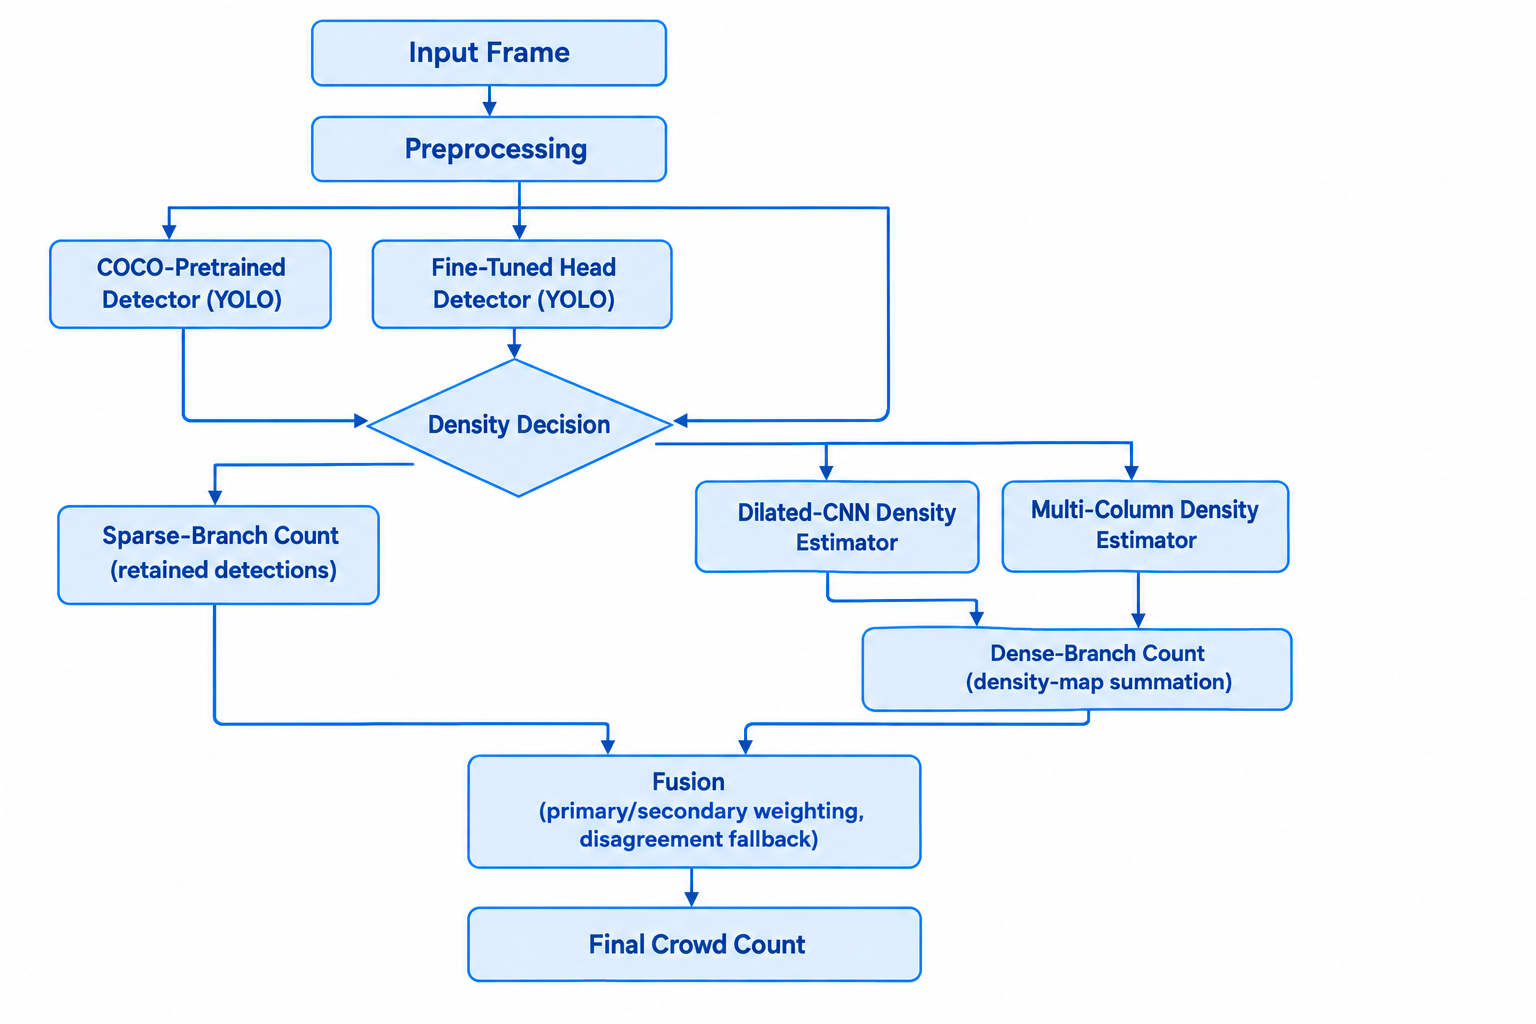
\includegraphics[width=0.92\textwidth]{./../images/pipeline_diagram.png}
	\caption{Architecture of the proposed adaptive hybrid crowd counting framework.}
	\label{fig:pipeline}
\end{figure}

The overall architecture is then five conceptual stages as illustrated in Figure~\ref{fig:pipeline}: (i) the input frame is passed to one or more candidate detector techniques; (ii) the outputs of the detector techniques are passed to a component that decides on whether the frame is sparse or dense based on the number of detections, detection density, and pairwise detection overlap; (iii) if the frame is dense, it is also passed to one of several candidate density estimation techniques, while if it is sparse, the detections are passed directly to a branch count component; (iv) both a sparse and a dense branch count are computed from the detections and passed to a (v) fusion component that reconciles the counts from the two branches into a single final crowd count, using one of several primary/secondary weighting schemes, with the secondary chosen whenever there is a strong disagreement between the two branches. 

\section{Data Analysis Techniques}
\label{sec:analysis-techniques}

As the sparse and dense branches produce structurally different outputs (discrete detections versus continuous density maps), and the classical, non-learned techniques (classical density estimation, density decision, fusion) are not trained against a loss function, each component of the framework is analysed with the metric family appropriate to its output.

\subsection{Image Pre-processing}

The preprocessor applies conditions on each frame before detection and density estimation using up to four optional, independently configurable stages, applied in sequence: resizing and scale normalization, non-local means denoising, Contrast Limited Adaptive Histogram Equalization (CLAHE) applied to the L-channel of the CIELAB colour space, and Gaussian smoothing. When a stage is disabled, its input passes through unchanged to the next stage.

\subsubsection{Resizing and Scale Normalization}

Before any denoising or contrast operation is applied, the raw frame $I_{raw}$ produced by input acquisition is resized to a standard working resolution:

\begin{equation}
	I_{in} = \operatorname{Resize}\left(I_{raw};\, \text{target}=w_{t},\, \text{interp}=\text{INTER\_AREA}\right), \qquad h_{t} = h_{raw} \cdot \frac{w_{t}}{w_{raw}}
	\label{eq:resize}
\end{equation}

where $w_t$ is the configured target width, $h_t$ the resulting target height, and the aspect ratio of the original frame $(w_{raw}, h_{raw})$ is preserved throughout. Area based interpolation is used because it is the theoretically appropriate choice for downscaling: unlike bilinear or nearest neighbour interpolation, which sample a fixed, small neighbourhood regardless of the scale change, area interpolation averages over the full block of source pixels each destination pixel covers, which reduces aliasing artefacts that would otherwise appear as spurious high frequency texture exactly the kind of artefact non-local means denoising would otherwise mistake for genuine, similarity matchable structure.

\subsubsection{Non-Local Means Denoising}

Non-local means denoising relies on the fact that in a crowd scene, similar texture and background regions occur many times throughout the image and the value of each pixel can be estimated by averaging with all the pixels in a search window where the surrounding patches are photometrically similar. denoised value of a pixel $p$ is

\begin{equation}
	I_{1}(p) = \frac{1}{C(p)} \sum_{q \in \Omega(p)} w(p,q)\, I_{in}(q)
	\label{eq:nlm-estimate}
\end{equation}
\begin{equation}
	w(p,q) = \exp\left(-\frac{\lVert N(p) - N(q) \rVert_2^2}{h^2}\right), \qquad C(p) = \sum_{q \in \Omega(p)} w(p,q)
	\label{eq:nlm-weight}
\end{equation}

The search window around $p$ ($\text{searchWindowSize}=21$), the local patches centred at $p$ and $q$ ($\text{templateWindowSize}=7$) used for similarity comparison, the filtering strength $h$ that controls the down weighting of dissimilar patches. In the case of colour images, denoising is done in the luminance chrominance decomposition with different strengths for luminance and colour channels, $h=3$ and $h_{color}=3$ respectively, respectively following the colour extension of the algorithm that suppress chroma noise without over smoothing brighteness edge. The spatial filter scheme, which depends only on the spatial distance between the two patches, does not preserve fine structure as well as the $w(p,q)$ scheme does because it does not consider similarity between the two patches.The fine structure (heads, edge of the occlusion boundary) is preserved better than a spatial filter scheme since the latter does not consider the similarity between the two patches. 

\subsubsection{Contrast Limited Adaptive Histogram Equalization}

\begin{equation}
	L' =
	\operatorname{CLAHE}\left(
	L;\,\text{clipLimit}=2.0,\,
	\text{tileGridSize}=8\times8
	\right)
	\label{eq:clahe}
\end{equation}

CLAHE partitions the $L$-channel into an $8\times8$ grid of contextual tiles, equalises the histogram within each tile, and clips histogram bins above a fixed limit (clipLimit $=2.0$) before redistributing the excess. This prevents noise over-amplification that plain histogram equalisation can introduce in near uniform regions. Operating in the perceptually motivated CIELAB space isolates luminance from chrominance, so that contrast enhancement does not distort colour. Applied to $I_1$ (or directly to $I_{in}$ if denoising is disabled), CLAHE improves local contrast in unevenly illuminated crowd scenes, such as shadowed platforms and backlit doorways. This enhancement can improve the recall of the downstream head/person detector, consistent with reported gains from CLAHE preprocessing in low contrast detection pipelines.

\subsubsection{Gaussian Smoothing}

\begin{equation}
	I_{out} =
	\operatorname{GaussianBlur}\left(
	I_{2};\,\text{kernel}=k_{blur},\,\sigma=0
	\right)
	\label{eq:gaussian-blur}
\end{equation}

A final, optional Gaussian smoothing pass with configurable kernel size $k_{blur}$ removes residual high-frequency artefacts introduced by CLAHE's per-tile equalisation before the frame is passed to the detection and density branches. Setting $\sigma=0$ allows the Gaussian standard deviation to be determined automatically from the selected kernel size.

\subsection{ShanghaiTech Dataset Preparation}

The ShanghaiTech dataset is prepared for density based crowd estimation using a dedicated preprocessing pipeline. Each image and its corresponding head annotations are resized to a fixed resolution of $768\times768$, with the annotation coordinates scaled accordingly. Ground truth density maps are generated by placing unit impulses at the annotated head locations and applying an adaptive Gaussian kernel whose standard deviation depends on the number of annotated heads. The resulting density maps are normalized to preserve the ground truth crowd count and subsequently downsampled by a factor of four to match the spatial resolution of the density estimation network. A scaling factor of $16$ is applied after downsampling to compensate for the reduction in spatial resolution. Input images are converted to RGB format and normalized to the range $[0,1]$. The resulting image density map pairs provide the supervision required for training the multi column density estimator.

\section{Proposed Algorithm}
\label{sec:proposed-algorithm}

\subsection{Overall Proposed Framework}

The overall workflow of the proposed adaptive hybrid crowd counting framework is summarized in Algorithm~\ref{alg:overall}. It integrates density-based scene decision, sparse detection, dense estimation, and count fusion into a unified pipeline as shows in Figure~\ref{fig:pipeline}.

\begin{algorithm}[H]
	\caption{Adaptive Hybrid Crowd Counting}
	\label{alg:overall}
	\begin{algorithmic}[1]
		\Require Video $V$ or a single frame $f$
		\Ensure Final crowd count $C$
		\For{each frame $f_t$}
		\State Preprocess $f_t$ for the selected detector technique (Section~\ref{sec:sparse})
		\State $\mathcal{D} \gets$ detections produced by the selected detector technique
		\State $s \gets$ \Call{DensityDecision}{$\mathcal{D}$, dimensions of $f_t$} \Comment{Section~\ref{sec:density-decision}}
		\State $C_{\text{sparse}} \gets |\mathcal{D}|$ (after any confidence/class filtering, Section~\ref{sec:sparse})
		\State Preprocess $f_t$ for the selected density estimation technique
		\State $\hat D \gets$ density map from the selected density estimation technique (Section~\ref{sec:dense})
		\State $C_{\text{dense}} \gets \sum \hat D$ \Comment{Equation~\ref{eq:density-sum}}
		\State $C_t \gets$ \Call{Fuse}{$s$, $C_{\text{sparse}}$, $C_{\text{dense}}$} \Comment{Section~\ref{sec:fusion}}
		\EndFor
		\State $C \gets$ aggregation of $\{C_1,\dots,C_n\}$ across frames 
		\State \Return $C$
	\end{algorithmic}
\end{algorithm}

Note that both the sparse branch count and the dense branch count are computed for every frame, regardless of the scene label $s$ assigned by the density decision component, $s$ determines which of the two counts the fusion component treats as primary rather than determining which branch is computed at all (Section~\ref{sec:fusion}).

\subsection{Head Detection}
\label{sec:sparse-detection}

Two candidate techniques were implemented for the detection role, spanning a general purpose pretrained deep detector, a domain-fine-tuned deep detector. All two produce a common output representation, a set of bounding boxes, each optionally carrying a confidence score which downstream components (density decision, sparse counting, fusion) consume identically regardless of which technique produced it.

\subsection{Sparse Scene Crowd Counting}
\label{sec:sparse}

\subsubsection{Pretrained General Purpose Detector}

The first sparse branch technique employs the pretrained YOLOv8m object detector as a general-purpose person detector, as illustrated in Fig.~\ref{fig:sparse_yolov8_pretrained}. The model is loaded using the Ultralytics detection framework and is used without additional training or fine-tuning. During inference, the detector is configured with an input image size of $1024$ pixels, a confidence threshold of $0.25$, and the person class (class $0$). Therefore, only detections classified as persons with confidence scores satisfying the specified threshold are retained for counting.

\begin{figure}[htbp]
	\centering
	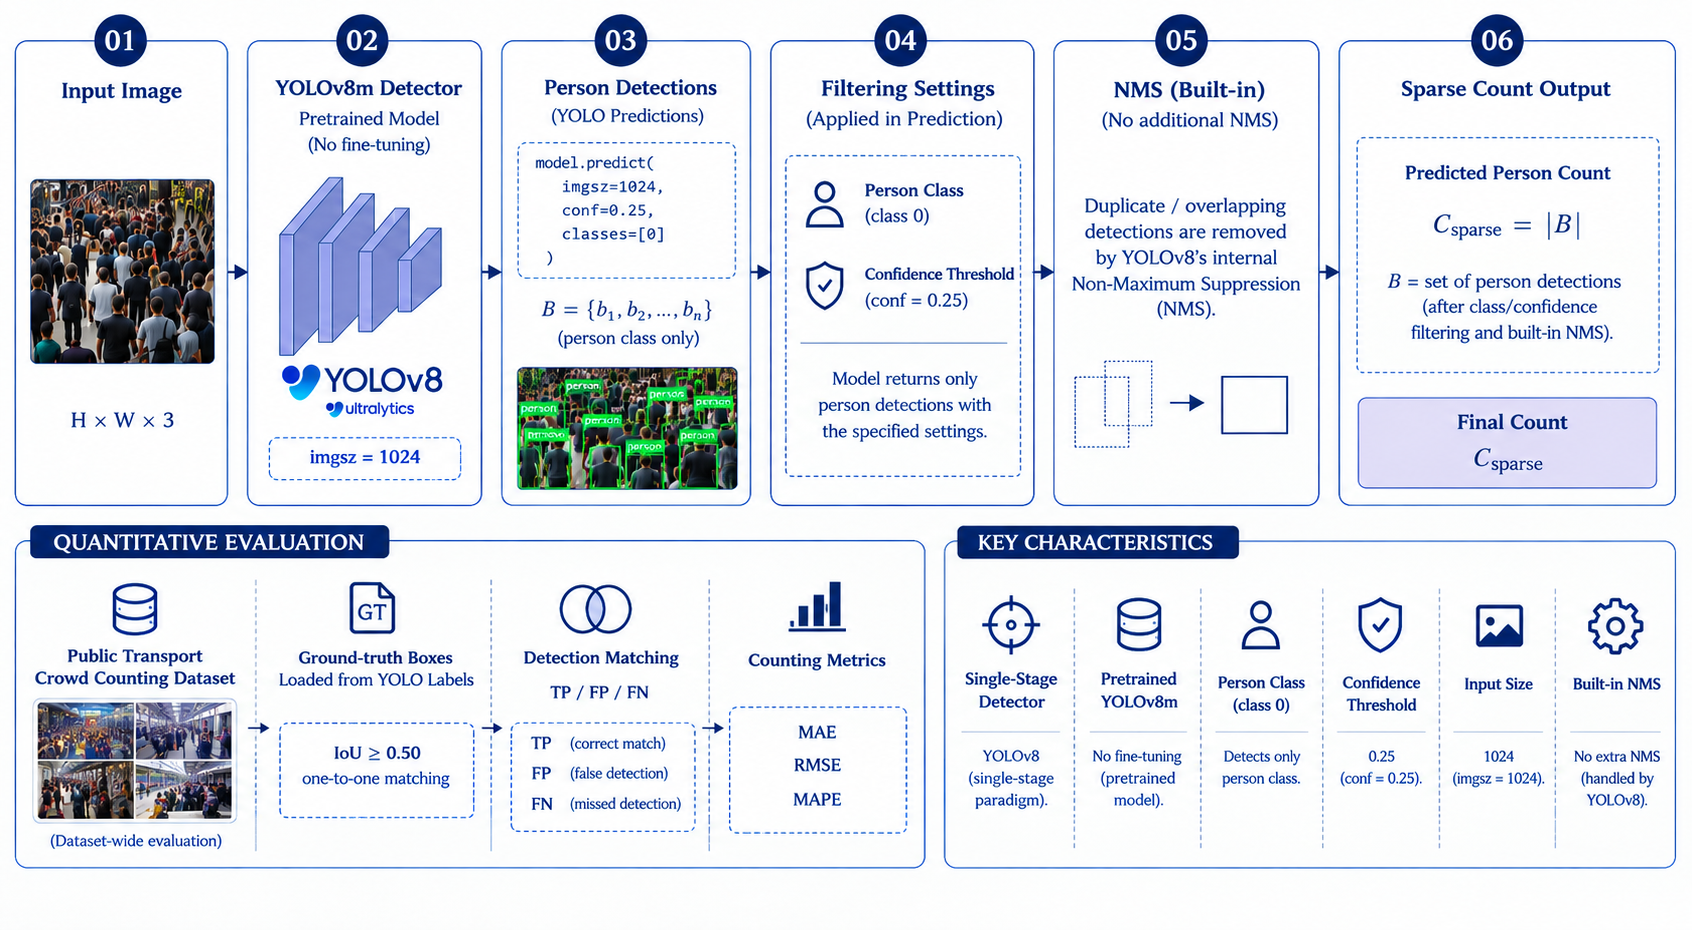
\includegraphics[width=\textwidth]{./../images/sparse/classical_yolo/architecture.png}
	\caption{Architecture of the pretrained YOLOv8 based sparse branch technique.}
	\label{fig:sparse_yolov8_pretrained}
\end{figure}

Let $B$ denote the set of bounding boxes returned by the pretrained YOLOv8m detector under the person class and confidence-threshold constraints. The sparse scene count is obtained directly from the number of retained detections:

\begin{equation}
C_{\text{sparse}} = |B|.
\end{equation}

The detector's built-in post-processing, including non-maximum suppression (NMS), is used to handle overlapping candidate detections, no additional NMS procedure is applied in the counting pipeline.

For quantitative evaluation, the predicted bounding boxes are compared with the ground truth bounding boxes provided with the public transport crowd counting dataset. A predicted box and a ground truth box are considered a match when their intersection-over-union (IoU) is at least $0.50$. A greedy one-to-one matching procedure is then used to determine true positives (TP), false positives (FP), and false negatives (FN). Based on these detections, precision, recall, and F1-score are calculated. In addition, counting performance is evaluated using the absolute counting error, mean absolute error (MAE), root mean squared error (RMSE), and mean absolute percentage error (MAPE).

\subsubsection{Fine Tuned Head Detector}

The second sparse branch technique fine tunes the pretrained YOLOv8m detector for single class head detection using the SCUT-HEAD dataset~\cite{peng2018scuthead}, as illustrated in Fig.~\ref{fig:sparse_yolov8_head}. The detector is initialized from the pretrained YOLO weights and fine tuned for 50 epochs with a batch size of 8 and an input image size of 1{,}280 pixels. Early stopping is enabled with a patience of 10 epochs, while a fixed random seed of 42 and deterministic training are used to improve reproducibility. The dataset contains a single object class, namely \textit{head} (class 0).

\begin{figure}[htbp]
	\centering
	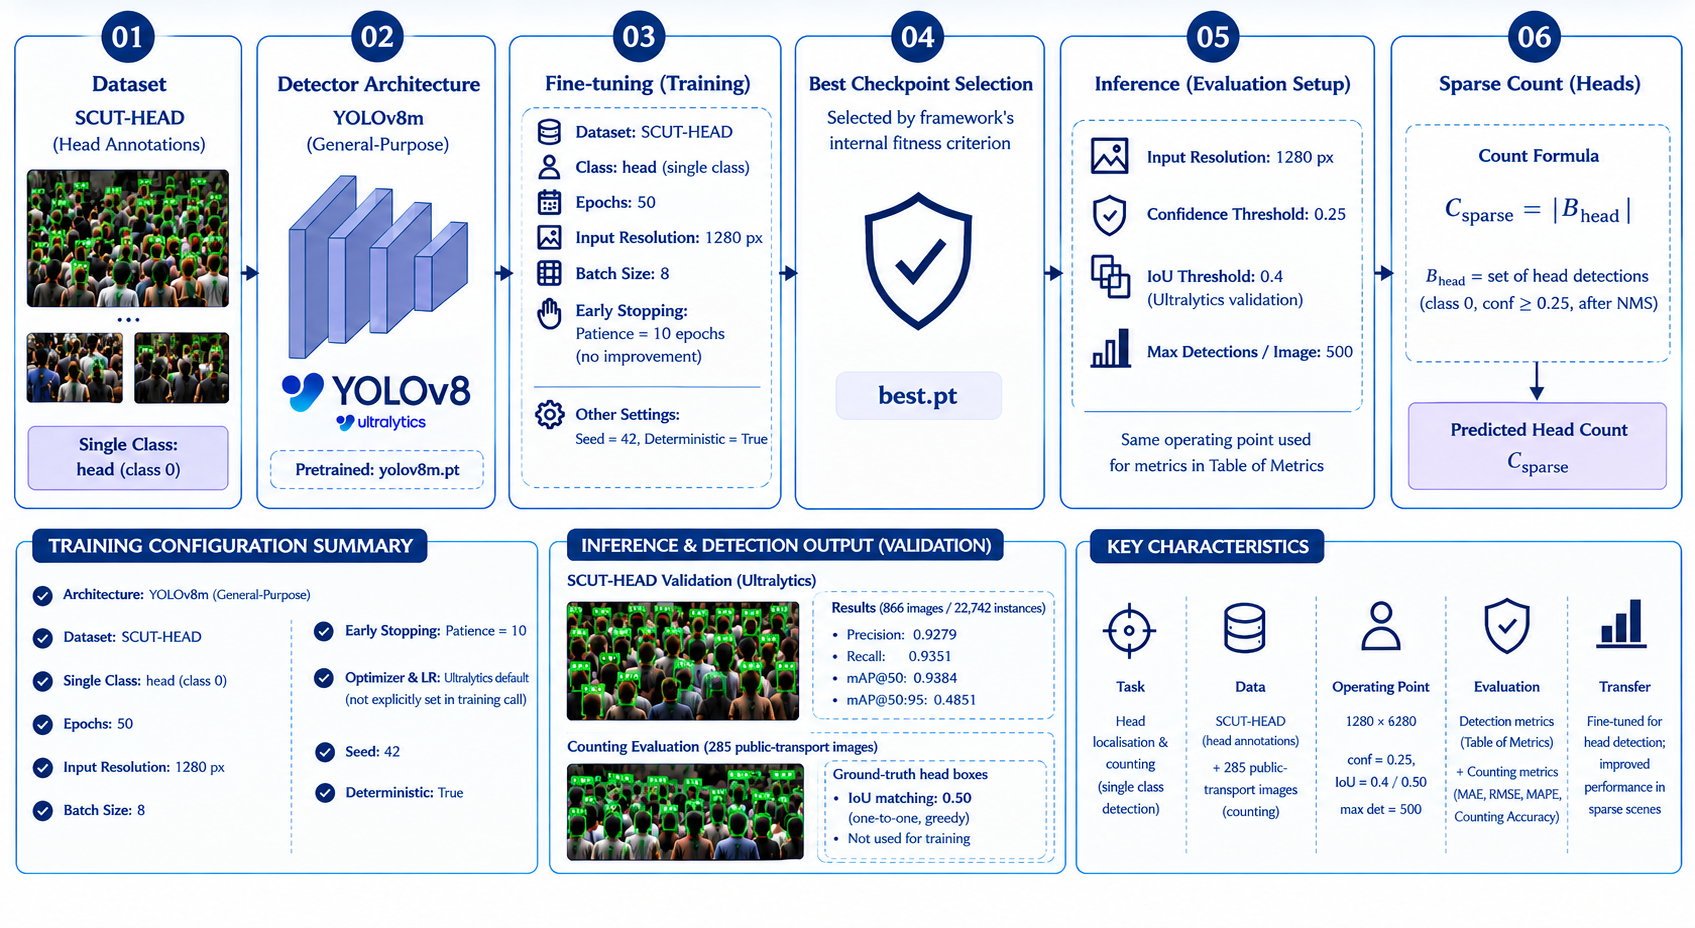
\includegraphics[width=\textwidth]{./../images/sparse/scut_head_yolo/architecture.png}
	\caption{Architecture of the fine tuned YOLOv8 head detection technique.}
	\label{fig:sparse_yolov8_head}
\end{figure}

The Ultralytics validation procedure is performed at an input resolution of 1{,}280 pixels with a batch size of 8, a confidence threshold of 0.25, an IoU threshold of 0.4, and a maximum of 500 detections per image.

For sparse scene counting, the number of detected heads is obtained directly from the retained detection boxes. Let $B_{\text{head}}$ denote the set of head detections returned by the fine tuned detector after the specified class and confidence filtering. The sparse scene count is then calculated as

\begin{equation}
    C_{\text{sparse}} = |B_{\text{head}}|.
\end{equation}

No additional non-maximum suppression is applied outside the YOLO detection framework.

\subsubsection{Comparison of Sparse Branch Techniques}
\label{sec:sparse-comparison}

Table~\ref{tab:sparse-compare} summarizes the main characteristics of these two sparse branch techniques and provides a basis for selecting an appropriate detector within the proposed hybrid framework.

\begin{longtable}{|
    >{\raggedright\arraybackslash}p{0.22\textwidth}|
    >{\raggedright\arraybackslash}p{0.38\textwidth}|
    >{\raggedright\arraybackslash}p{0.32\textwidth}|}

\caption{Comparison of the two sparse branch (detection-based) techniques.}
\label{tab:sparse-compare}\\

\hline
\textbf{Aspect} &
\textbf{Pretrained Detector} &
\textbf{Fine-Tuned Detector} \\
\hline
\endfirsthead

\multicolumn{3}{c}%
{{\tablename\ \thetable{} -- continued from previous page}} \\
\hline
\textbf{Aspect} &
\textbf{Pretrained Detector} &
\textbf{Fine-Tuned Detector} \\
\hline
\endhead

\hline
\multicolumn{3}{r}{{Continued on next page}} \\
\endfoot

\hline
\endlastfoot

Underlying method
&
Deep, single stage regression detector~\cite{redmon2016yolo}
&
Same architecture, fine tuned
\\
\hline

Training performed
&
None (pretrained weights only)
&
Fine tuning, 50 epochs
\\
\hline

Target class
&
Person (general)
&
Head (domain specific)
\\
\hline

Confidence output
&
Graded score
&
Graded score
\\
\hline

Quantitative evaluation
&
None (qualitative only)
&
Detection metrics (Table~\ref{tab:metrics})
\\
\hline

\end{longtable}

\subsection{Density Decision}
\label{sec:density-decision}

The density decision component determines whether a frame is treated as sparse or dense, using only the detections produced by the upstream detector and the frame's spatial dimensions, it does not itself re-examine pixel content. Given a detection set $\mathcal{D} = \{d_1,\dots,d_n\}$ and a frame of height $h$ and width $w$, the component first normalises the frame area into units of 1{,}000 pixels$^2$,

\begin{equation}
	a = \frac{h \cdot w}{1000},
\end{equation}

and then applies a two stage rule. First, if the number of detections falls below a configured minimum threshold $\tau_{\min}$, the frame is classified as sparse immediately, without computing density or overlap (an efficiency short circuit for frames that are trivially uncrowded):

\begin{equation}
	n < \tau_{\min} \;\Rightarrow\; \text{scene} = \text{sparse}.
\end{equation}

Otherwise, two indicators are computed. The first is a detection \emph{density}, expressed as detections per 1{,}000 pixels$^2$ of frame area,

\begin{equation}
	\rho = \frac{n}{a} \qquad (a>0),
\end{equation}

and the second is a pairwise \emph{overlap ratio}, defined as the fraction of all unordered detection pairs whose bounding boxes have a nonzero Intersection-over-Union:

\begin{equation}
	\text{IoU}(d_i,d_j) = \frac{|\,\text{box}(d_i) \cap \text{box}(d_j)\,|}{|\,\text{box}(d_i) \cup \text{box}(d_j)\,|}, \qquad
	r = \frac{\bigl|\{(d_i,d_j) : \text{IoU}(d_i,d_j) > 0\}\bigr|}{\binom{n}{2}} \quad (n \ge 2),
\end{equation}

with $r = 0$ defined for $n<2$. The Intersection-over-Union quantity itself is the standard overlap measure used in object detection matching and non-maximum suppression is used not to suppress duplicate detections but to gauge how crowded (mutually occluding) the detected individuals are. The frame is classified as dense if either indicator exceeds its configured threshold,

\begin{equation}
	\rho \ge \tau_{\rho} \;\;\text{or}\;\; r \ge \tau_{r} \;\Rightarrow\; \text{scene} = \text{dense}, \qquad \text{otherwise scene} = \text{sparse},
\end{equation}

where $\tau_{\rho}$ (a density threshold, in detections per 1{,}000 pixels$^2$) and $\tau_{r}$ (an overlap ratio threshold in $[0,1]$) are configured constants. This rule means a frame can be classified dense either because it contains many detections relative to its area, or because a large fraction of its detections mutually overlap, even if the absolute detection count is moderate, capturing two distinct visual symptoms of crowding (numerosity and occlusion) with a single decision. 

\subsection{Dense Scene Crowd Counting}
\label{sec:dense}

\subsubsection{Ground truth density maps}

For each training image, a ground truth density map is constructed by placing a unit impulse at each annotated head location after rescaling the annotation coordinates to the network's fixed input resolution of $768{\times}768$. The resulting point map is smoothed using a Gaussian filter with a standard deviation

\begin{equation}
	\sigma =
	\begin{cases}
		0.5\,\sigma_{\text{base}}, & N > 100 \\
		\sigma_{\text{base}}, & N \le 100
	\end{cases}
	\qquad \sigma_{\text{base}} = 5,
\end{equation}

where $N$ is the number of annotated heads in the image. Thus, images containing more than 100 annotated heads use $\sigma=2.5$, whereas images with 100 or fewer heads use $\sigma=5$. After Gaussian smoothing, the density map is renormalised so that its total mass equals the ground truth head count $N$. The density map is subsequently downsampled by a factor of four to match the spatial resolution of the network output. Because the downsampling factor is four in each spatial dimension, the density values are multiplied by $4^2=16$ to compensate for the spatial reduction.

\subsubsection{Multi Column Density Estimator}
\label{sec:fourcolumn-density}

\begin{figure}[htbp]
	\centering
	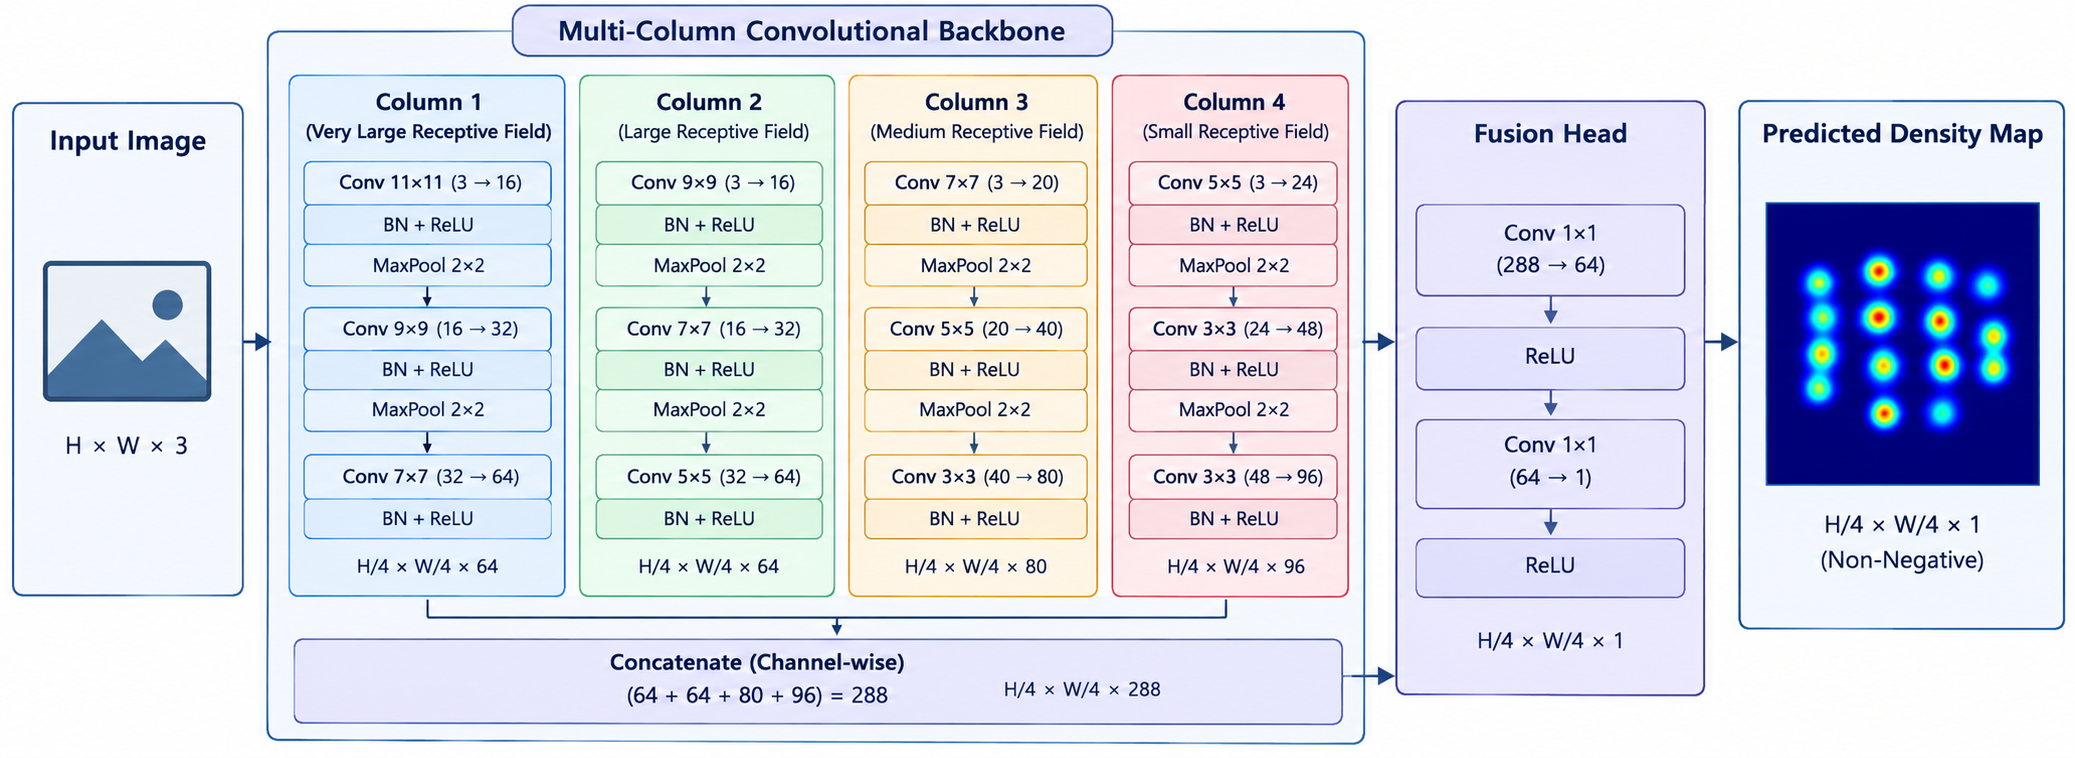
\includegraphics[width=\textwidth]{./../images/dense/mcnn/architecture.png}
	\caption{Architecture of Multi Column Density Estimator}
	\label{fig:multi_column_architecture}
\end{figure}

The first learned density estimation method is along the lines of the multi column convolutional architecture introduced by ~\cite{Zhu2020} (see Figure~\ref{fig:multi_column_architecture}) where multiple stacked parallel convolutional columns are trained on the same image, where each column uses a different kernel size to learn features for a different range of head sizes due to perspective and scale variations. Four parallel columns are used, with progressively smaller kernel sizes across the columns: the first column uses kernel sizes $11/9/7$, the second uses $9/7/5$, the third uses $7/5/3$, and the fourth uses $5/3/3$. The channel widths increase across the columns, with the four branches producing 64, 64, 80, and 96 output channels, respectively. Each convolution is followed by batch normalisation and ReLU activation, while two $2{\times}2$ max-pooling operations in each column reduce the spatial resolution by a factor of four. Thus, for the fixed input resolution of $768{\times}768$, all four branches produce feature maps of spatial size $192{\times}192$. The four feature maps are concatenated channel-wise, producing 304 channels, and are then passed through a fusion head consisting of a $1{\times}1$ convolution that reduces the channels from 304 to 64, followed by ReLU, and a second $1{\times}1$ convolution that produces a single channel output. A final ReLU ensures non-negative density values, yielding the predicted density map $\hat D$.

\subsubsection{Dilated Convolution Density Estimator}
\label{sec:csrnet-density}

\begin{figure}[htbp]
	\centering
	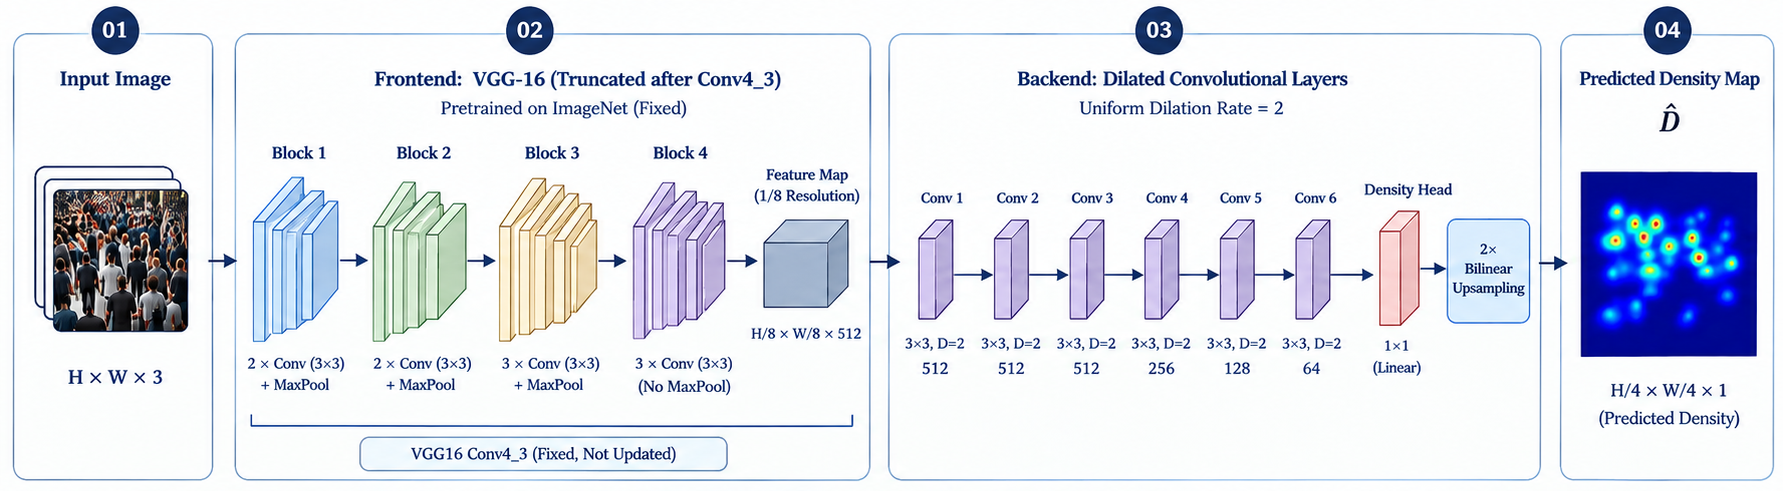
\includegraphics[width=\textwidth]{./../images/dense/csrnet/architecture.png}
	\caption{Architecture of Dilated Convolution Density Estimator.}
	\label{fig:csrnet_architecture}
\end{figure}

The second learned density estimation technique follows a two-part frontend and backend design based on the CSRNet architecture for congested scene density regression, as illustrated in Figure~\ref{fig:csrnet_architecture}. The frontend is based on a VGG16 convolutional network pretrained on ImageNet. The VGG16 feature extractor is truncated after the \texttt{conv4\_3} layer, corresponding to the fourth convolutional block. The frontend reduces the spatial resolution of the input from $768 \times 768$ to $96 \times 96$, while the pretrained frontend parameters are frozen during training and are therefore not updated.

The backend consists of six $3{\times}3$ convolutional layers with a uniform dilation rate of 2 and output channel sizes of 512, 512, 512, 256, 128, and 64. The dilated convolutions enlarge the receptive field while maintaining the $96{\times}96$ spatial resolution. A final $1{\times}1$ convolution reduces the 64 channel feature representation to a single channel density map. The predicted density map is subsequently upsampled by a factor of 2 using bilinear interpolation, producing a final spatial resolution of $192{\times}192$.

\subsubsection{Training}

The network is trained from randomly initialised weights using the Adam optimiser with an initial learning rate of $1\times10^{-4}$ and a batch size of 8. A StepLR learning rate scheduler is used with a step size of 10 epochs and a multiplicative factor of 0.1. Training is configured for a maximum of 100 epochs with early stopping using a patience of 30 epochs, and the checkpoint with the lowest validation loss is retained as the best model. The training objective is a weighted combination of pixel wise density map error and count level error,

\begin{equation}
	\mathcal{L} = 0.9 \, \mathcal{L}_{\text{MSE}}(\hat D, D) + 0.1 \, \bigl|{\textstyle\sum}\hat D - N_{gt}\bigr|,
\end{equation}

where the count level loss is computed using the absolute difference between the predicted and ground truth counts. For an individual sample, the predicted count is obtained by summing all values in the predicted density map,

\begin{equation}
	\hat C=\sum_{x,y}\hat D(x,y),
\end{equation}

and the count loss is

\begin{equation}
	\mathcal{L}_{\text{count}}=|\hat C-N_{\text{gt}}|.
\end{equation}

For a training batch, the implemented $\mathrm{L1Loss}$ computes the mean absolute count error across the samples. Input images are converted to RGB, resized to $768{\times}768$, and normalised to the range $[0,1]$ by division by 255, without additional channel-wise normalisation. No image augmentation is applied in the training configuration.

\subsubsection{Comparison of Dense Branch Techniques}
\label{sec:dense-comparison}

Table~\ref{tab:dense-compare} compares the two dense branch techniques in terms of their architectural design, density estimation capability, computational complexity, and overall suitability for handling variations in crowd density.

\begin{longtable}{|
	>{\raggedright\arraybackslash}p{0.22\textwidth}|
	>{\raggedright\arraybackslash}p{0.36\textwidth}|
	>{\raggedright\arraybackslash}p{0.34\textwidth}|}

\caption{Comparison of the two dense branch (density estimation) techniques.}
\label{tab:dense-compare}\\

\hline
\textbf{Aspect} &
\textbf{Multi-column Estimator} &
\textbf{Dilated CNN Estimator} \\
\hline
\endfirsthead

\multicolumn{3}{c}%
{{\tablename\ \thetable{} -- continued from previous page}} \\
\hline
\textbf{Aspect} &
\textbf{Multi-column Estimator} &
\textbf{Dilated CNN Estimator} \\
\hline
\endhead

\hline
\multicolumn{3}{r}{{Continued on next page}} \\
\endfoot

\hline
\endlastfoot

Underlying method
&
Multi-column CNN~\cite{Zhu2020}
&
VGG frontend + dilated backend
\\
\hline

Learned parameters
&
Yes (trained from scratch)
&
Yes (frontend pretrained and frozen; backend trained)
\\
\hline

Depends on a detector
&
No
&
No
\\
\hline

ground truth smoothing $\sigma$
&
Adaptive: 5 or 2.5 by crowd size
&
Fixed: 4
\\
\hline

Training loss
&
$0.9\,\mathcal{L}_{\mathrm{MSE}} + 0.1\,\left|\sum \hat{D} - N_{\mathrm{gt}}\right|$
&
$\mathcal{L}_{\mathrm{MSE}}$ only
\\
\hline

\end{longtable}

\subsection{Fusion and Final Crowd Count}
\label{sec:fusion}

The fusion component reconciles the sparse branch count $C_{\text{sparse}}$ and the dense branch count $C_{\text{dense}}$, both of which are computed for every frame regardless of the scene label $s$ assigned by the density decision component, into a single final count for that frame. The scene label determines which of the two branch counts is treated as primary and which as secondary:

\begin{equation}
	(P,S) =
	\begin{cases}
		(C_{\text{sparse}}, C_{\text{dense}}), & s = \text{sparse} \\
		(C_{\text{dense}}, C_{\text{sparse}}), & s = \text{dense}
	\end{cases}
\end{equation}

with corresponding weights $(w_P,w_S)$ drawn analogously from a pair of configured branch weights (a sparse weight and a dense weight). If the primary count is non positive, the fusion component falls back to whichever of the two counts is larger, avoiding a zero final count when the primary branch reports nothing but the secondary branch has positive signal:

\begin{equation}
	P \le 0 \;\Rightarrow\; C = \max(P,S).
\end{equation}

Otherwise, a relative disagreement between the two branches is computed,

\begin{equation}
	\Delta = \frac{|P-S|}{P},
\end{equation}

and if this disagreement exceeds a configured threshold $\tau_{\Delta}$, the branches are judged too discordant to blend meaningfully, and the fusion component reports the primary count alone, trusting the branch that the density decision component identified as authoritative for that frame:

\begin{equation}
	\Delta > \tau_{\Delta} \;\Rightarrow\; C = P.
\end{equation}
Otherwise, the final count is a weighted average of the two branch counts,
\begin{equation}
	\Delta \le \tau_{\Delta} \;\Rightarrow\; C = \frac{P\,w_P + S\,w_S}{w_P + w_S}.
\end{equation}

The reason for this design is that the fusion component only blends the two branches where they are in reasonable agreement, and does not blend two potentially incommensurate density estimates, but rather just defers to the branch the density decision chose to take the lead.

\subsection{Evaluation Metrics}
\label{subsec:evaluation-metrics}

The evaluation strategy uses metrics appropriate to each component of the proposed crowd counting framework. The sparse detection branch is assessed using precision, recall, mAP@50, and mAP@50:95, while the learned density estimators are evaluated using pixel wise MSE, MAE, and count level MAE. The classical density estimator and deterministic density fusion components do not require training based metrics; instead, their outputs are assessed through diagnostic counts and fixed decision rules. Table~\ref{tab:metrics} summarizes the evaluation approach for each component.

\begin{longtable}{|
		>{\raggedright\arraybackslash}p{0.24\textwidth}|
		>{\raggedright\arraybackslash}p{0.33\textwidth}|
		>{\raggedright\arraybackslash}p{0.33\textwidth}|}
	
	\caption{Evaluation approach by component.}
	\label{tab:metrics}\\
	
	\hline
	\textbf{Component} &
	\textbf{Quantitative Evaluation Implemented} &
	\textbf{Notes} \\
	\hline
	\endfirsthead
	
	\multicolumn{3}{c}%
	{{\tablename\ \thetable{} -- continued from previous page}} \\
	\hline
	\textbf{Component} &
	\textbf{Quantitative Evaluation Implemented} &
	\textbf{Notes} \\
	\hline
	\endhead
	
	\hline
	\multicolumn{3}{r}{{Continued on next page}} \\
	\endfoot
	
	\hline
	\endlastfoot
	
	Pretrained sparse detector
	&
	Precision, recall, mAP@50, mAP@50:95
	&
	Single image, qualitative demonstration only
	\\
	\hline
	
	Fine tuned sparse detector
	&
	Precision, recall, mAP@50, mAP@50:95
	&
	Standard detection metrics at a fixed confidence/IoU operating point
	\\
	\hline
		
	Dilated CNN density estimator
	&
	Pixel wise MSE (training loss), pixel wise MAE, and custom count level MAE
	&
	Count level MAE compares summed predicted and ground truth density maps per batch
	\\
	\hline
	
	Multi column density estimator
	&
	Combined pixel wise MSE $+$ count level MAE (training loss); count level MAE tracked separately
	&
	Weighted combination, with weights fixed in the implementation
	\\
	\hline
	
\end{longtable}

\subsubsection{Count Based Evaluation Metrics}

For the sparse and dense branch evaluation, the following whole image count metrics are used, with $\hat c_i$ the predicted count and $c_i$ the ground truth count for image $i$ of $M$ evaluated images:

\begin{equation}
	\text{MAE} = \frac{1}{M}\sum_{i=1}^{M} \left| \hat{c}_i - c_i \right|, \qquad
	\text{RMSE} = \sqrt{ \frac{1}{M}\sum_{i=1}^{M} \left( \hat{c}_i - c_i \right)^2 }
\end{equation}

\begin{equation}
	\text{MAPE} = \frac{1}{M}\sum_{i=1}^{M} \frac{\left| \hat{c}_i - c_i \right|}{c_i} \times 100\%, \qquad
	\text{Bias} = \frac{1}{M}\sum_{i=1}^{M} \left( \hat{c}_i - c_i \right)
\end{equation}

RMSE penalises large individual errors more heavily than MAE, so a wide MAE/RMSE gap indicates that error is concentrated in a minority of images rather than spread evenly. Bias indicates systematic direction: a negative value indicates the model under counts on average. All four metrics are lower-is-better; bias is exceptional in that its \emph{sign}, not only its magnitude, is informative.

\subsubsection{Detection Metrics (Fine Tuned Sparse Detector)}

Detection quality is evaluated using precision ($P$), recall ($R$), and mean Average Precision (mAP), computed from matched predicted and ground truth bounding boxes. The evaluation follows the object detection protocol formalised for the PASCAL Visual Object Classes challenge. In this study, detection performance is evaluated using a confidence threshold of 0.25, an Intersection-over-Union (IoU) threshold of 0.4, and a maximum of 500 detections per image. These settings are applied to the best checkpoint obtained during fine tuning.

\textbf{Precision} measures the proportion of predicted head boxes that correspond to ground truth heads. It is defined as:

\begin{equation}
	P = \frac{TP}{TP + FP},
\end{equation}

where $TP$ (true positives) represents the number of predicted boxes that sufficiently overlap with a ground truth head, while $FP$ (false positives) represents predictions that do not correspond to a ground truth head. Higher precision indicates fewer spurious detections.

\textbf{Recall} measures the proportion of ground truth heads that are successfully detected. It is defined as:

\begin{equation}
	R = \frac{TP}{TP + FN},
\end{equation}

where $FN$ (false negatives) represents the number of ground truth heads for which no corresponding prediction is obtained. Higher recall indicates fewer missed heads.

\textbf{Mean Average Precision (mAP)} provides a comprehensive measure of detection performance by summarising precision across the range of confidence thresholds. For \textbf{mAP@50}, Average Precision (AP) is calculated at a single IoU threshold of 0.50. The IoU between a predicted bounding box $A$ and a ground truth bounding box $B$ is defined as:

\begin{equation}
	\text{IoU}(A,B) = \frac{|A \cap B|}{|A \cup B|},
\end{equation}

while Average Precision is expressed as:

\begin{equation}
	\text{AP} = \int_0^1 p(r),dr,
\end{equation}

where $p(r)$ represents precision as a function of recall $r$.

The \textbf{mAP@50} metric therefore measures Average Precision at an IoU threshold of 0.50. In contrast, \textbf{mAP@50:95} averages AP across ten IoU thresholds from 0.50 to 0.95 in steps of 0.05. Consequently, mAP@50:95 provides a stricter and more localisation sensitive assessment of detection performance than mAP@50. For all three metrics, higher values indicate better detection performance.

\subsubsection{Density Estimation Training Metrics (Learned Dense Branch Estimators)}

Both learned density estimation techniques are trained with a pixel wise error term between the predicted density map $\hat D$ and the ground truth density map $D$,

\begin{equation}
	\mathcal{L}_{\text{MSE}} = \frac{1}{N_p}\sum_{i=1}^{N_p}\left(\hat D_i - D_i\right)^2,
\end{equation}

where $N_p$ is the number of cells in the (downsampled) density map. In addition, both techniques track a count level error metric that compares the summed predicted and ground truth density maps rather than their per-pixel values, expressed for a batch of size $B$ as

\begin{equation}
	\text{count\_MAE} = \frac{1}{B}\sum_{b=1}^{B}\left|\sum_{i} D_{b,i} - \sum_{i} \hat D_{b,i}\right|.
\end{equation}

This count level metric is used because pixel wise error on a density map is difficult to interpret directly in terms of people counted; expressing error in the same units as the final deliverable (a count) makes model comparison more directly meaningful. One of the two learned estimators uses only the pixel wise MSE as its training loss (with pixel wise MAE and count level MAE tracked as auxiliary metrics), while the other combines the pixel wise MSE and the count level error directly into its training loss (Section~\ref{sec:dense}).

\subsubsection{Count Derivation from a Density Map}

For any density estimation technique, learned or classical, the predicted crowd count $\hat C$ for a frame is obtained by spatial summation of the predicted density map,

\begin{equation}
	\hat C = \sum_{i=1}^{N_p} \hat D_i .
	\label{eq:density-sum}
\end{equation}

This relationship holds for the two learned estimators (where it is used directly in computing the count level MAE metric above) and, in a closed form variant, for the classical estimator.

\chapterpage{Results Analysis and Discussion}
\mychapter{Results Analysis and Discussion}
\label{chap:results}

In this chapter, the empirical evidence given by the different components of the proposed adaptive hybrid crowd counting framework (pretrained classic person detector, head detector fine tuned on the SCUT Head dataset, custom four column density regression network, the dilated convolution density network style of the CSRNet and a classical detection assisted density estimation procedure) is presented and analysed.

\section{Data Collection and Analysis}

The techniques explored in this study have two categories represented by three annotated datasets. The learned techniques (the fine tuned sparse detector and the two dense density map estimators) are trained, fine tuned and validated with SCUT-HEAD and ShanghaiTech, Part~B, respectively for sparse and dense branch. The role played by the Public Transport Crowd Counting Dataset (PTCCD) is quite different, instead of training or fine tuning any of the individual techniques, it is used to test the performance of the proposed, fully populated passenger counting framework under realistic transportation conditions. Table~\ref{tab:datasets} briefly summarises the three datasets used, and provides information about their role, while Table~\ref{tab:dataset-stats} reports detailed size, split, and annotation density statistics as reported by the original sources.

\begin{longtable}{|
    >{\raggedright\arraybackslash}p{0.24\textwidth}|
    >{\raggedright\arraybackslash}p{0.21\textwidth}|
    >{\raggedright\arraybackslash}p{0.18\textwidth}|
    >{\raggedright\arraybackslash}p{0.24\textwidth}|
}
\caption{Datasets used for training and evaluation.}
\label{tab:datasets}\\
\hline
\textbf{Dataset} &
\textbf{Annotation type} &
\textbf{Used by} &
\textbf{Role} \\
\hline
\endfirsthead

\hline
\textbf{Dataset} &
\textbf{Annotation type} &
\textbf{Used by} &
\textbf{Role} \\
\hline
\endhead

\hline
\endfoot

\hline
\endlastfoot

SCUT-HEAD~\cite{peng2018scuthead} &
Head bounding boxes (YOLO text format) &
Fine tuned sparse detector &
Fine tuning and validation (detection metrics) \\
\hline

ShanghaiTech, Part B~\cite{Zhu2020} &
Head point locations (\texttt{.mat} files) &
Both learned dense branch estimators &
Training and validation (density map / count metrics) \\
\hline

Public Transport Crowd Counting Dataset (PTCCD) &
Passenger/head bounding boxes (YOLO text format) &
Proposed passenger counting framework (full pipeline) &
Held out evaluation only, not used for training or fine tuning any individual technique \\
\hline

\end{longtable}

\begin{longtable}{|
		>{\raggedright\arraybackslash}p{0.18\textwidth}|
		>{\raggedright\arraybackslash}p{0.09\textwidth}|
		>{\raggedright\arraybackslash}p{0.18\textwidth}|
		>{\raggedright\arraybackslash}p{0.15\textwidth}|
		>{\raggedright\arraybackslash}p{0.24\textwidth}|}
	
	\caption{Detailed dataset statistics}
	\label{tab:dataset-stats}\\
	
	\hline
	\textbf{Dataset} &
	\textbf{Images} &
	\textbf{Train / Test / Val} &
	\textbf{Annotated instances} &
	\textbf{Notes} \\
	\hline
	\endfirsthead
	
	\multicolumn{5}{c}%
	{{\tablename\ \thetable{} -- continued from previous page}} \\
	\hline
	\textbf{Dataset} &
	\textbf{Images} &
	\textbf{Train / Test / Val} &
	\textbf{Annotated instances} &
	\textbf{Notes} \\
	\hline
	\endhead
	
	\hline
	\multicolumn{5}{r}{{Continued on next page}} \\
	\endfoot
	
	\hline
	\endlastfoot
	
	SCUT-HEAD, Part~A~\cite{peng2018scuthead}
	&
	2{,}000
	&
	1{,}100 / 500 / 400
	&
	67{,}318 heads
	&
	Classroom surveillance imagery, low inter image variance by design
	\\
	\hline
	
	SCUT-HEAD, Part~B~\cite{peng2018scuthead}
	&
	2{,}329
	&
	1{,}630 / 233 / 466
	&
	41{,}749 heads
	&
	Internet crawled imagery, higher visual variability
	\\
	\hline
	
	SCUT-HEAD, combined
	&
	4{,}329
	&
	2{,}730 / 733 / 866
	&
	109{,}067 heads
	&
	Union of Part~A and Part~B, as used for fine tuning in this study
	\\
	\hline
	
	ShanghaiTech, Part~B~\cite{Zhu2020}
	&
	716
	&
	400 / 316
	&
	88{,}272 heads (point-annotated)
	&
	Fixed resolution $768{\times}1024$, approximately 9--578 people per image, mean $\approx 123.6$
	\\
	\hline

	Public Transport Crowd Counting Dataset (PTCCD)
	&
	285
	&
	--
	&
	Approx. 8{,}311 passengers/heads (bounding box annotated)\footnotemark
	&
	Variable resolution; 2--60 annotated objects per image, mean $\approx 29.16$, median 29; used for framework level evaluation only, not split into train/test
	\\
	\hline
	
\end{longtable}

\subsubsection{SCUT HEAD Dataset}
The fine tuned sparse detector is trained on SCUT-HEAD, a head detection dataset comprising 4{,}329 images with 109{,}067 annotated head bounding boxes~\cite{peng2018scuthead}. The dataset is collected in two parts that differ in imaging condition and scene variability:

\begin{itemize}
	\item \textbf{Part A:} 2{,}000 images sampled from classroom surveillance video within a single university, with 67{,}318 heads annotated; because classroom scenes recur with limited pose variation, the constituent images were deliberately selected to maximise representative variance. As distributed, Part~A is pre-split into 1{,}100 training, 400 validation, and 500 testing images.
	\item \textbf{Part B:} 2{,}329 images crawled from the internet, with 41{,}749 heads annotated, offering greater visual diversity than Part~A. As distributed, Part~B is pre-split into 1{,}630 training, 466 validation, and 233 testing images.
\end{itemize}

Every annotated head is bounded by an axis aligned box $(x_{\min}, y_{\min}, x_{\max}, y_{\max})$ covering the full head extent, including occluded portions, without extraneous background, following the Pascal VOC annotation convention. In the implementation examined for this study, Part~A and Part~B are pooled into a single combined dataset of 4{,}329 images (2{,}730 for training, 733 for testing) while each image's original split membership is preserved, and a single object class (head) is declared, since the study task is class agnostic head localisation rather than the finer classroom versus internet distinction that motivated the dataset's original two part structure.

\subsubsection{ShanghaiTech Dataset, Part B}
Both learned density estimation techniques are trained and evaluated on Part~B of the ShanghaiTech crowd counting dataset, introduced alongside the multi column convolutional architecture on which one of the two density estimators is based~\cite{Zhu2020}. ShanghaiTech as a whole comprises 1{,}198 images with 329{,}547 annotated head points, split into a dense, internet sourced Part~A (482 images) and a sparser, street-level Part~B (716 images); this study uses Part~B only. Part~B images are all captured at a fixed resolution of $768{\times}1024$ pixels on busy Shanghai streets, officially divided into 400 training and 316 testing images, with per-image counts ranging from approximately 9 to 578 people and a mean of approximately 123.6 people per image, substantially sparser than Part~A (mean $\approx$501 people per image), which was not used in this study. Annotations are provided as a single $(x,y)$ pixel coordinate per head, stored per image in a MATLAB \texttt{.mat} file, rather than as bounding boxes. Both density estimation techniques uses only the official 400-image training subset: a fixed, seeded 90/10 split is drawn from it, giving 360 images for training and holding out the remaining 40 for validation during training; this same 40-image held-out set is subsequently reused as the evaluation set for reported test metrics, so the official 316-image test subset is not used by this technique. During training, this technique additionally applies random-crop augmentation, so the network is fed fixed-size image and density-map crops rather than full frames, whereas the held-out validation/test images are processed at their full $768{\times}1024$ resolution; in both cases the target density map is downsampled by a factor of 8 relative to the input. The other technique uses the official test subset directly as its validation set during training, without a further internal split. Point annotations are not used directly as supervision; both techniques convert them into smoothed density maps prior to training, as described in Section~\ref{sec:dense}.


\subsubsection{Public Transport Crowd Counting Dataset}
\label{sec:ptccd}

Unlike SCUT-HEAD and ShanghaiTech, Part~B, the Public Transport Crowd Counting Dataset (PTCCD) is not used to train or fine tune any individual technique in this study. Instead, it is used to evaluate the performance of the proposed passenger counting framework as a whole, in realistic transportation environments. The dataset contains a total of 285 images and 285 corresponding annotation files, resulting in a one-to-one correspondence between images and labels. The images represent different passenger configurations and crowd densities, making the dataset suitable for evaluating both sparse and relatively dense passenger-counting conditions.

The number of annotated objects in each image was calculated from the corresponding label file. For every annotation file, the number of non-empty annotation lines was counted. The resulting statistics are shown in Table~\ref{tab:object_statistics}.

\begin{longtable}{|l|c|}
\caption{Statistics of Annotated Objects per Image}
\label{tab:object_statistics} \\
\hline
\textbf{Statistic} & \textbf{Number of Objects} \\
\hline
\endfirsthead

\multicolumn{2}{|c|}{%
\textbf{\tablename\ \thetable{} -- continued from previous page}} \\
\hline
\textbf{Statistic} & \textbf{Number of Objects} \\
\hline
\endhead

\hline
\multicolumn{2}{|r|}{\textit{Continued on next page}} \\
\hline
\endfoot

\hline
\endlastfoot

Minimum & 2 \\
\hline
Maximum & 60 \\
\hline
Mean & 29.16 \\
\hline
Median & 29.00 \\
\hline

\end{longtable}

The dataset contains an average of 29.16 annotated objects per image, with a median of 29 objects and a range of 2 to 60 objects. This variation represents different passenger density conditions and helps evaluate the model's robustness across varying crowd sizes.

\begin{figure}[htbp]
    \centering
    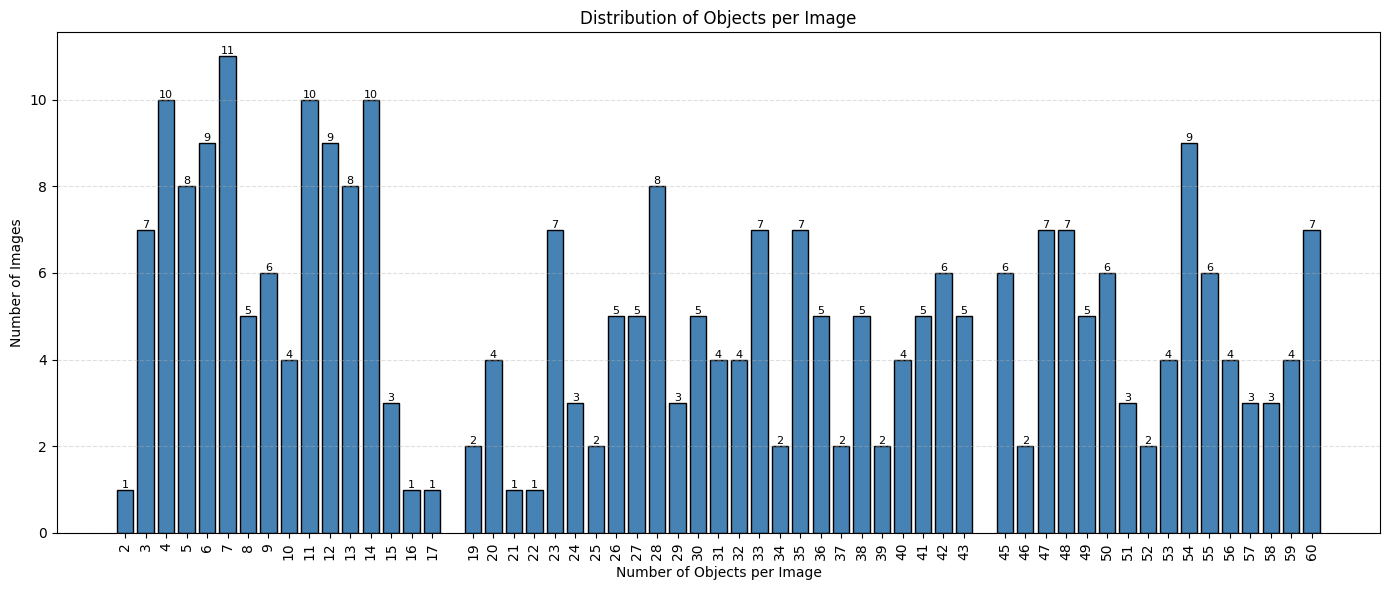
\includegraphics[width=1.0\textwidth]
    {./../images/ptccd_image_distribution.png}
	\caption{Annotated objects per image}
    \label{fig:object_distribution}
\end{figure}

The object count distribution illustrates the variation in the number
of annotated passengers across the dataset. It provides an overview of
the typical crowd size and the spread of passenger counts among the
images.

\begin{figure}[htbp]
    \centering
    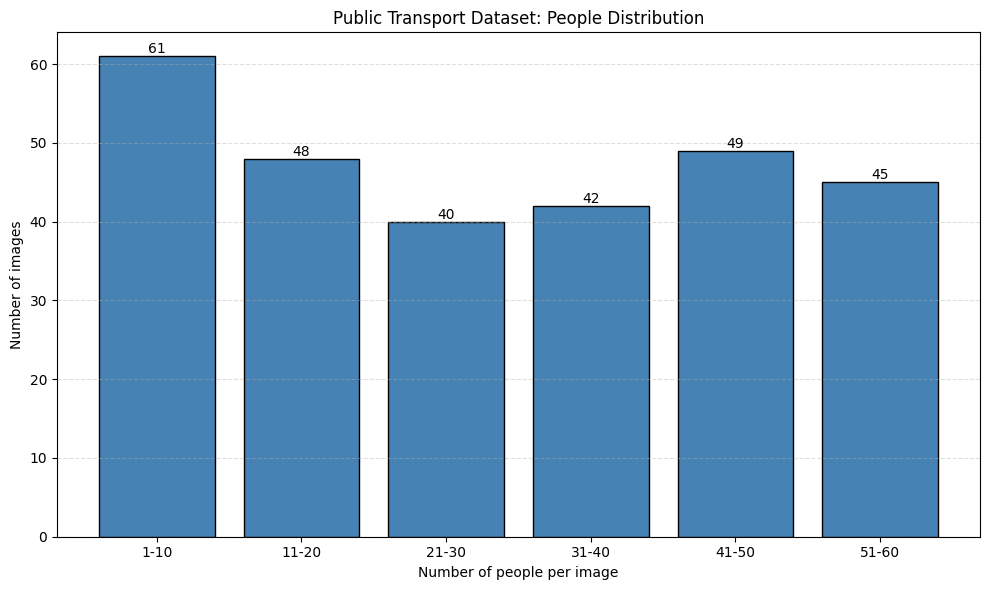
\includegraphics[width=0.9\textwidth]
    {./../images/ptccd_range_distribution.png}
	\caption{Image distribution by annotated object count.}
    \label{fig:range_crowd_distribution}
\end{figure}

The range wise grouping provides a simple way to examine whether the
dataset is concentrated around a particular crowd density level or
contains a broad range of passenger counts. The resulting distribution
is shown in Figure~\ref{fig:range_crowd_distribution}.

\section{Interpretation of Results}

\subsection{Classic YOLO: Pretrained Detector}
\label{sec:classic_yolo}

This section reports the experimental results obtained from applying a pretrained, off the shelf YOLO object detector to head counting on the public transport crowd counting(285 image) test set used in the preceding experiments. Detections were obtained using the model's default (pretrained) weights with inference parameters \textit{imgsz=1024}, \textit{conf=0.25}, restricted to \textit{classes=[0]} (the COCO ``person'' category). As the pretrained model was optimised to localise whole body person instances rather than heads, a systematic geometric mismatch between predicted and ground truth bounding boxes is expected \textit{a priori}, independent of the detector's underlying ability to identify the presence of individuals. The results reported below are interpreted with this expectation as the analytical baseline.

\subsubsection{Quantitative Detection Based Counting Performance}

Table~\ref{tab:pretrained_yolo_summary} presents the overall detection performance of the pretrained YOLO detector on the 285 image test set. The very low precision, recall, and F1 score at IoU = 0.50 do not necessarily mean that the detector fails to identify people. The main issue is the difference between the annotations and the detector output: the ground truth contains small head only boxes, while the pretrained model produces boxes covering the full person. As a result, a correct person detection may have very little overlap with the corresponding head annotation and therefore be counted as a false positive. The low number of true positives is therefore mainly due to this mismatch between the evaluation annotations and the detector's output format.


\begin{longtable}{|
>{\raggedright\arraybackslash}p{0.65\textwidth}|
>{\raggedright\arraybackslash}p{0.27\textwidth}|
}

\caption{Pretrained YOLO counting performance on test set.}
\label{tab:pretrained_yolo_summary} \\

\hline
\textbf{Metric} & \textbf{Value} \\
\hline
\endfirsthead

\multicolumn{2}{|c|}{%
\textit{\tablename\ \thetable{} -- continued from previous page}} \\
\hline

\textbf{Metric} & \textbf{Value} \\
\hline
\endhead

\hline
\multicolumn{2}{|c|}{\textit{Continued on next page}} \\
\hline
\endfoot

\hline
\endlastfoot

Images & 285 \\
\hline
Total Ground Truth & 8{,}310 \\
\hline
Total Predictions & 6{,}709 \\
\hline
True Positives (IoU 0.50) & 145 \\
\hline
False Positives (IoU 0.50) & 6{,}564 \\
\hline
False Negatives (IoU 0.50) & 8{,}165 \\
\hline
Precision @ IoU 0.50 & 0.0216 \\
\hline
Recall @ IoU 0.50 & 0.0174 \\
\hline
F1-score @ IoU 0.50 & 0.0193 \\
\hline
Mean Ground Truth Count & 29.16 \\
\hline
Mean Predicted Count & 23.54 \\
\hline
Mean Absolute Error (MAE) & 8.81 \\
\hline
Root Mean Squared Error (RMSE) & 12.18 \\
\hline
Mean Absolute Percentage Error (MAPE) & 32.18\% \\
\hline

\end{longtable}

The count level results in Table~\ref{tab:pretrained_yolo_summary} and Figure~\ref{fig:pretrained_yolo_actual_predicted} show that the pretrained YOLO detector performs poorly when its bounding boxes are compared with the head annotations using IoU = 0.50. However, the predicted person counts still show a strong relationship with the actual crowd counts. This suggests that, although the detector does not match the head annotations well at the bounding box level, it can still provide useful information about the number of people in an image.

\begin{figure}[htbp]
	\centering
	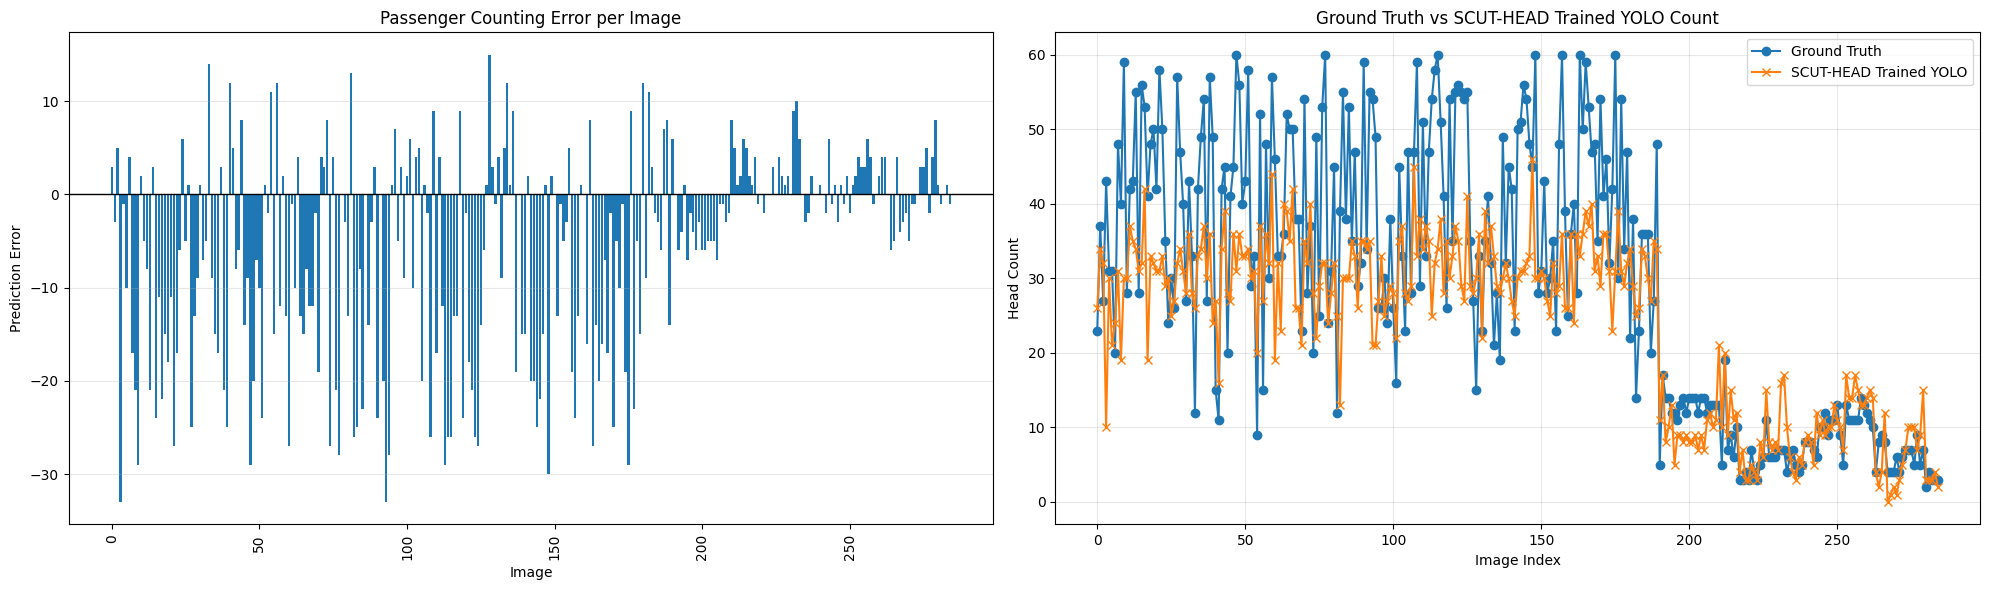
\includegraphics[width=1.0\linewidth]{./../images/sparse/classical_yolo/per_image_error_and_gt_vs_predicted.png}
	\caption{Pretrained YOLO counting error and predictions.}
	\label{fig:pretrained_yolo_actual_predicted}
\end{figure}

The counting error shown in Figure~\ref{fig:pretrained_yolo_actual_predicted} is mainly biased toward underestimation: the detector undercounts in 167 of the 285 test images, overcounts in 98, and is exact in 20. This is likely due to occlusion in crowded scenes, where people overlap with each other and their full body bounding boxes can overlap heavily. As a result, non-maximum suppression may remove some detections even when multiple people are present. In contrast, heads can remain visible even when much of the body is hidden. Therefore, the undercounting is mainly related to the use of whole body detection in crowded scenes rather than a problem specific to this model.

These results show that fine tuning should focus on adapting the detector to the head based annotations rather than simply improving its ability to detect people. As discussed in Section~\ref{sec:scut_yolo}, the main issue is the mismatch between whole person predictions and head based ground truth. The largest counting errors occurred in crowded images, where the detector returned fewer than half of the annotated individuals (for example, 10 detections for a ground truth count of 43, and 21 for 54), showing that heavy occlusion can cause severe undercounting as people overlap. This further highlights the need for a head-based detector in crowded scenes.

\subsubsection{Detection Based Counting Performance by Ground Truth Count Range}

The results across the six ground truth count ranges in Table~\ref{tab:pretrained_yolo_range_breakdown} and Figure~\ref{fig:pretrained_yolo_range_metrics} show that absolute counting error generally increases as the crowd becomes larger, from a MAE of 2.69 in the 1--10 range to 22.44 in the 51--60 range. However, percentage error is highest in images with fewer people (45.84\% for 1--10) because even a small counting mistake has a larger effect when the ground truth count is low. Counting accuracy is highest in the moderately populated ranges (21--30 and 31--40), where the crowd is large enough to reduce the effect of individual errors but not so dense that occlusion causes major detection problems.

\begin{figure}[htbp]
	\centering
	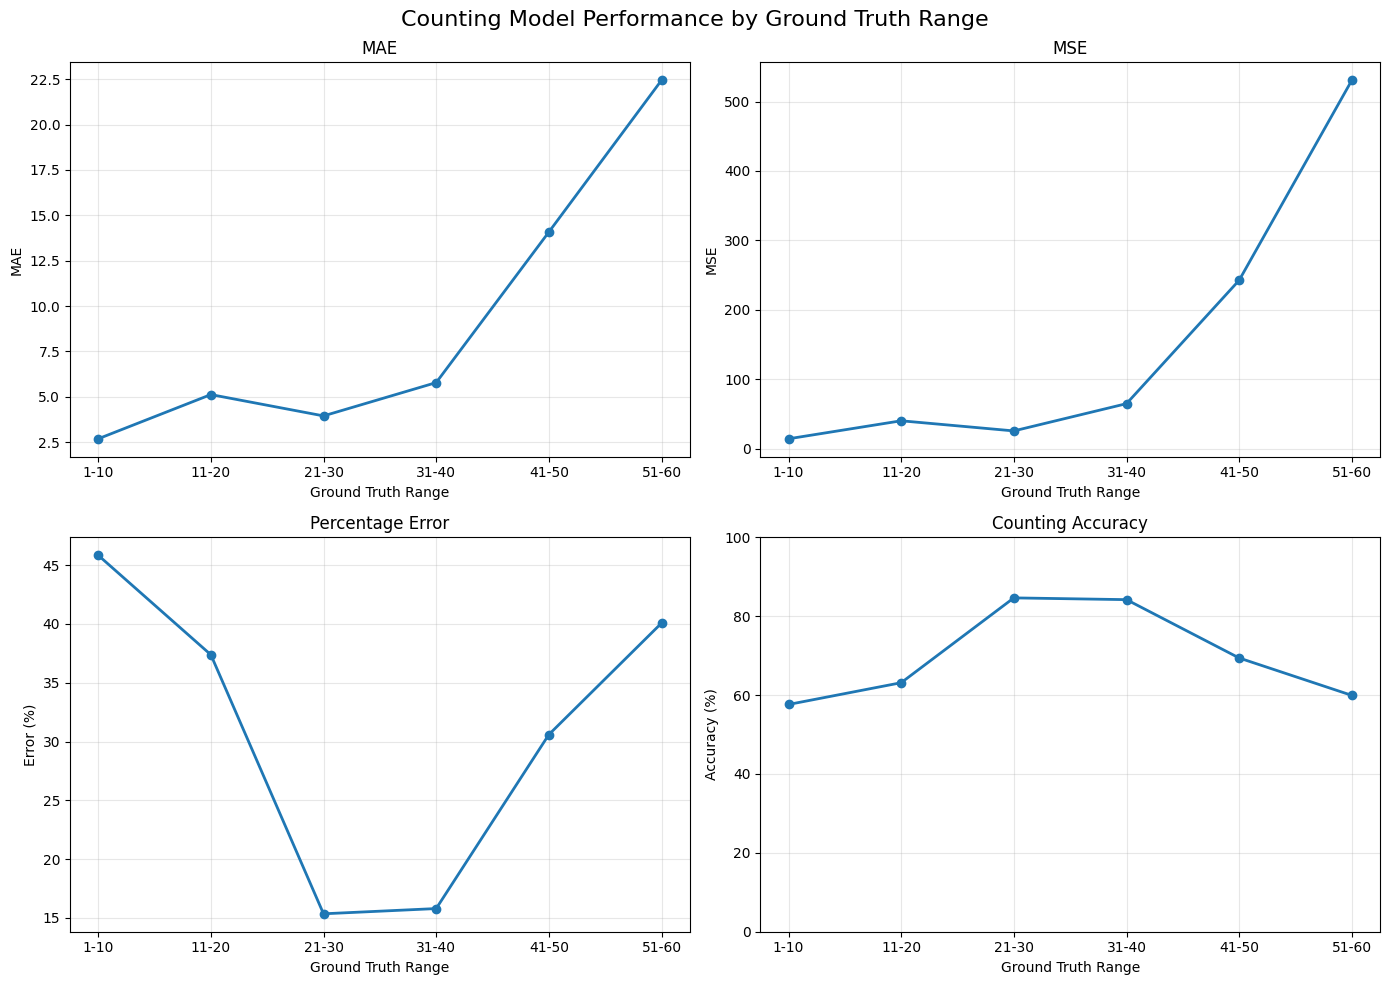
\includegraphics[width=1.0\linewidth]{./../images/sparse/classical_yolo/performance_by_gt_range.png}
	\caption{Pretrained YOLO performance across ground truth count ranges.}
	\label{fig:pretrained_yolo_range_metrics}
\end{figure}

The counting bias changes with crowd density. In images with up to 30 people, the bias is small and slightly positive, indicating that the whole body detector performs reasonably well when people are mostly visible. From the 31--40 range onward the bias becomes negative and grows rapidly (reaching $-22.44$ in the 51--60 range), showing progressively greater undercounting as occlusion increases. This suggests that crowd density has a direct effect on the detector's ability to count people accurately.

\begin{longtable}{|
    >{\raggedright\arraybackslash}p{0.08\textwidth}|
    >{\centering\arraybackslash}p{0.04\textwidth}|
    >{\centering\arraybackslash}p{0.10\textwidth}|
    >{\centering\arraybackslash}p{0.10\textwidth}|
    >{\centering\arraybackslash}p{0.10\textwidth}|
    >{\centering\arraybackslash}p{0.14\textwidth}|
    >{\centering\arraybackslash}p{0.12\textwidth}|
    >{\centering\arraybackslash}p{0.10\textwidth}|
}
\caption{Pretrained YOLO counting performance by ground truth count range}
\label{tab:pretrained_yolo_range_breakdown} \\
\hline
\textbf{GT Range} & $\boldsymbol{n}$ & \textbf{MAE} & \textbf{RMSE} &
\textbf{Mean \% Error} & \textbf{Mean Acc. (\%)} &
\textbf{Mean Bias} & \textbf{Mean F1} \\
\hline
\endfirsthead

\multicolumn{8}{|c|}%
{{\tablename\ \thetable{} -- continued from previous page}} \\
\hline
\textbf{GT Range} & $\boldsymbol{n}$ & \textbf{MAE} & \textbf{RMSE} &
\textbf{Mean \% Error} & \textbf{Mean Acc. (\%)} &
\textbf{Mean Bias} & \textbf{Mean F1} \\
\hline
\endhead

\hline
\multicolumn{8}{|c|}{{Continued on next page}} \\
\hline
\endfoot

\hline
\endlastfoot

1--10  & 61 & \textbf{2.6885} & \textbf{3.7417} & 45.8424 & 57.6210 & 1.3115 & 0.0970 \\
\hline
11--20 & 48 & 5.1250 & 6.3213 & 37.3815 & 63.1393 & 1.7917 & \textbf{0.1417} \\
\hline
21--30 & 40 & 3.9500 & 5.0349 & \textbf{15.3537} & \textbf{84.6463} & 2.8500 & 0.0011 \\
\hline
31--40 & 42 & 5.7857 & 8.0401 & 15.7987 & 84.2013 & $-4.3571$ & 0.0050 \\
\hline
41--50 & 49 & 14.0816 & 15.5721 & 30.5932 & 69.4068 & $-14.0408$ & 0.0000 \\
\hline
51--60 & 45 & 22.4444 & 23.0372 & 40.0734 & 59.9266 & $-22.4444$ & 0.0024 \\
\hline

\end{longtable}

Box level detection performance is highest at low densities (mean F1 of 0.0970 and 0.1417 for the 1--10 and 11--20 ranges, respectively) and is close to zero for all ranges above 20 people. This is mainly caused by the mismatch between whole person predictions and head level annotations, which becomes more severe when people are heavily occluded. As crowd density increases, it becomes harder for whole body boxes to achieve an IoU of 0.50 with the smaller head annotations.

These results show that the pretrained detector's counting performance depends on crowd density. It performs better in low to moderate density scenes but degrades in high density scenes. This density related pattern is not clear from the overall box level metrics, which remain very low across the test set.

\subsection{SCUT-Head YOLO: Fine Tuned Head Detector}
\label{sec:scut_yolo}

This section reports the experimental results obtained from training and evaluating a YOLO based object detector on the SCUT Head dataset for head detection, and from using this detector as a head counting mechanism on the same 285 image test set used in the preceding density estimation experiments.

\subsubsection{Training Performance and Convergence}

Detection performance is already relatively high at the first training epoch (precision 0.895, recall 0.833, mAP@50 0.890) because the network uses transfer learning from a COCO pretrained model. Instead of learning detection from the beginning, the model starts with existing detection knowledge and adapts it to the head specific annotations. Therefore, the training process mainly improves the model's existing detection ability to match the smaller head bounding boxes rather than learning object detection from scratch.

\begin{figure}[htbp]
	\centering
	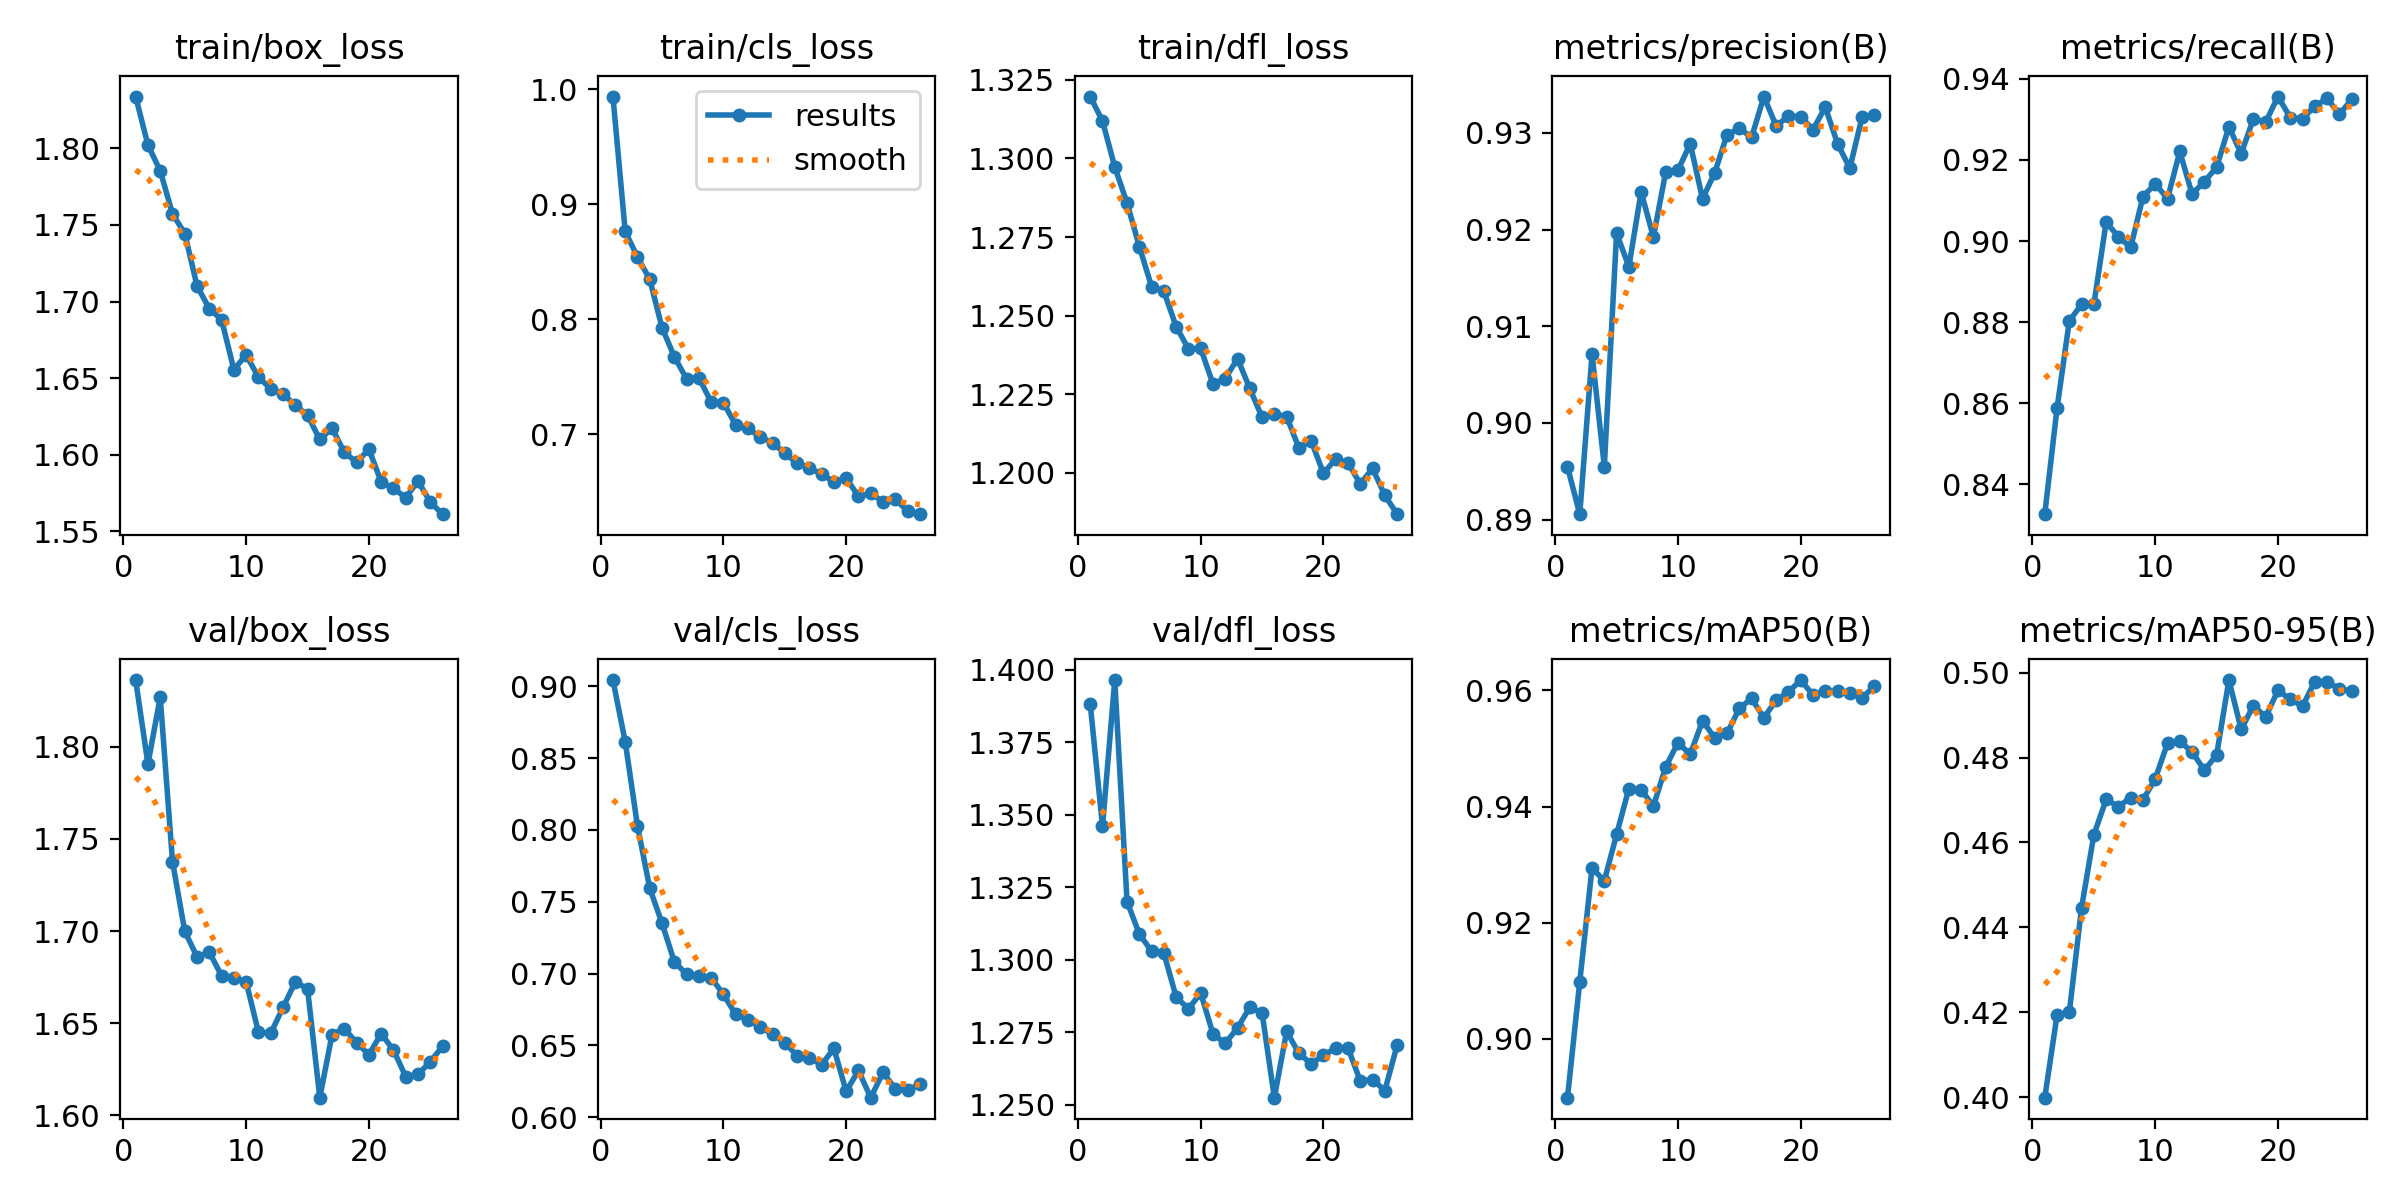
\includegraphics[width=1.0\linewidth]{./../images/sparse/scut_head_yolo/results.png}
	\caption{YOLO head detector training losses and detection metrics}
	\label{fig:scut_head_yolo_training_curves}
\end{figure}

Figure~\ref{fig:scut_head_yolo_training_curves} shows the training and validation losses together with the main detection metrics across the 26 training epochs. All three training losses decrease steadily over the run (box loss from 1.834 to 1.561, classification loss from 0.9936 to 0.6306, and distribution focal loss from 1.32 to 1.187), whereas the corresponding validation losses each reach a minimum earlier in training (box and distribution focal loss at epoch 16, classification loss at epoch 22) and subsequently fluctuate within a narrow band without further sustained improvement. Although the run was configured for 50 epochs, training stopped early after 26 epochs, indicating that the early stopping criterion was met before the maximum number of epochs was reached. This indicates that the model achieves most of its generalisation performance before the end of training, with later training mainly improving the fit to the training data.

\begin{longtable}{
		|>{\centering\arraybackslash}p{3.0cm}
		|>{\centering\arraybackslash}p{1.4cm}
		|>{\centering\arraybackslash}p{1.4cm}
		|>{\centering\arraybackslash}p{1.7cm}
		|>{\centering\arraybackslash}p{1.4cm}
		|>{\centering\arraybackslash}p{1.8cm}
		|>{\centering\arraybackslash}p{2.0cm}|
	}
	\caption{YOLO head detector training progression summary on SCUT-Head at key epochs}
	\label{tab:scut_head_yolo_training_summary}\\
	
	\hline
	\textbf{Epoch} &
	\textbf{Train Box} &
	\textbf{Val Box} &
	\textbf{Precision} &
	\textbf{Recall} &
	\textbf{mAP@50} &
	\textbf{mAP@50--95} \\
	\hline
	\endfirsthead
	
	\multicolumn{7}{|c|}{%
		\textbf{\tablename\ \thetable{} -- continued from previous page}%
	} \\
	\hline
	\textbf{Epoch} &
	\textbf{Train Box} &
	\textbf{Val Box} &
	\textbf{Precision} &
	\textbf{Recall} &
	\textbf{mAP@50} &
	\textbf{mAP@50--95} \\
	\hline
	\endhead
	
	\hline
	\multicolumn{7}{|r|}{\textit{Continued on next page}} \\
	\hline
	\endfoot
	
	\hline
	\endlastfoot
	
	1 (initial)
	& 1.8338
	& 1.8362
	& 0.8954
	& 0.8326
	& 0.8898
	& 0.3999 \\
	\hline
	
	16 (best mAP@50--95)
	& 1.6100
	& \textbf{1.6096}
	& 0.9295
	& 0.9282
	& 0.9586
	& \textbf{0.4982} \\
	\hline
	
	26 (final)
	& \textbf{1.5612}
	& 1.6374
	& 0.9319
	& 0.9349
	& 0.9608
	& 0.4957 \\
	\hline
	
\end{longtable}

As shown in Figure~\ref{fig:scut_head_yolo_training_curves} and Table~\ref{tab:scut_head_yolo_training_summary}, the detection metrics reach their best values within a narrow range of epochs (epochs 16--20), indicating stable convergence. Validation mAP@50--95 peaks at 0.498 at epoch 16, precision at 0.934 at epoch 17, and recall and mAP@50 at 0.936 and 0.962 at epoch 20. After approximately epoch 20, validation performance shows little further improvement, while training loss continues to decrease. The final epoch (mAP@50 of 0.961 and mAP@50--95 of 0.496) remains close to the best performance, suggesting that the additional training was mainly computationally redundant rather than harmful.

\subsubsection{Quantitative Detection Based Counting Performance}

The fine tuned YOLO detector shows a substantial improvement in precision, recall, and F1 score (0.4449, 0.4273, and 0.4359, respectively) on the same 285 image test set, as reported in Table~\ref{tab:scut_head_yolo_summary}. This improvement results from adapting the model to the head level annotations, resolving the geometric mismatch identified in Section~\ref{sec:classic_yolo}. The detection metrics remain moderate because head bounding boxes are small, meaning even a small error in box position or size can cause a prediction to fall below the IoU 0.50 threshold. Thus, some remaining errors are related to localisation accuracy rather than complete detection failures.

\begin{longtable}{|
>{\raggedright\arraybackslash}p{0.65\textwidth}|
>{\raggedright\arraybackslash}p{0.27\textwidth}|
}

\caption{YOLO head detector counting performance}
\label{tab:scut_head_yolo_summary} \\

\hline
\textbf{Metric} & \textbf{Value} \\
\hline
\endfirsthead

\multicolumn{2}{|c|}{%
\textit{\tablename\ \thetable{} -- continued from previous page}} \\
\hline

\textbf{Metric} & \textbf{Value} \\
\hline
\endhead

\hline
\multicolumn{2}{|c|}{\textit{Continued on next page}} \\
\hline
\endfoot

\hline
\endlastfoot

Images & 285 \\
\hline

Total Ground Truth & 8{,}310 \\
\hline

Total Predictions & 7{,}982 \\
\hline

True Positives (IoU 0.50) & 3{,}551 \\
\hline

False Positives (IoU 0.50) & 4{,}431 \\
\hline

False Negatives (IoU 0.50) & 4{,}759 \\
\hline

Precision @ IoU 0.50 & 0.4449 \\
\hline

Recall @ IoU 0.50 & 0.4273 \\
\hline

F1-score @ IoU 0.50 & 0.4359 \\
\hline

Mean Ground Truth Count & 29.16 \\
\hline

Mean Predicted Count & 28.01 \\
\hline

Mean Absolute Error (MAE) & 2.8491 \\
\hline

Root Mean Squared Error (RMSE) & 4.2501 \\
\hline

Mean Absolute Percentage Error (MAPE) & 15.55\% \\
\hline

\end{longtable}

The count level results in Table~\ref{tab:scut_head_yolo_summary} and Figure~\ref{fig:scut_head_yolo_actual_predicted} show that the fine tuned detector provides more accurate and reliable counting than the pretrained model, with stronger correlation and lower counting errors. The remaining negative counting bias (a mean error of $-1.15$ heads per image, with 7{,}982 heads predicted against 8{,}310 in the ground truth, a 3.9\% undercount) indicates some undercounting: 150 of the 285 images are undercounted, 98 are overcounted, and 37 are counted exactly. The reduced magnitude of this bias suggests that head specific training has partially reduced the occlusion related detection problem. However, performance can still decrease in very dense scenes where heads are heavily occluded.

\begin{figure}[htbp]
	\centering
	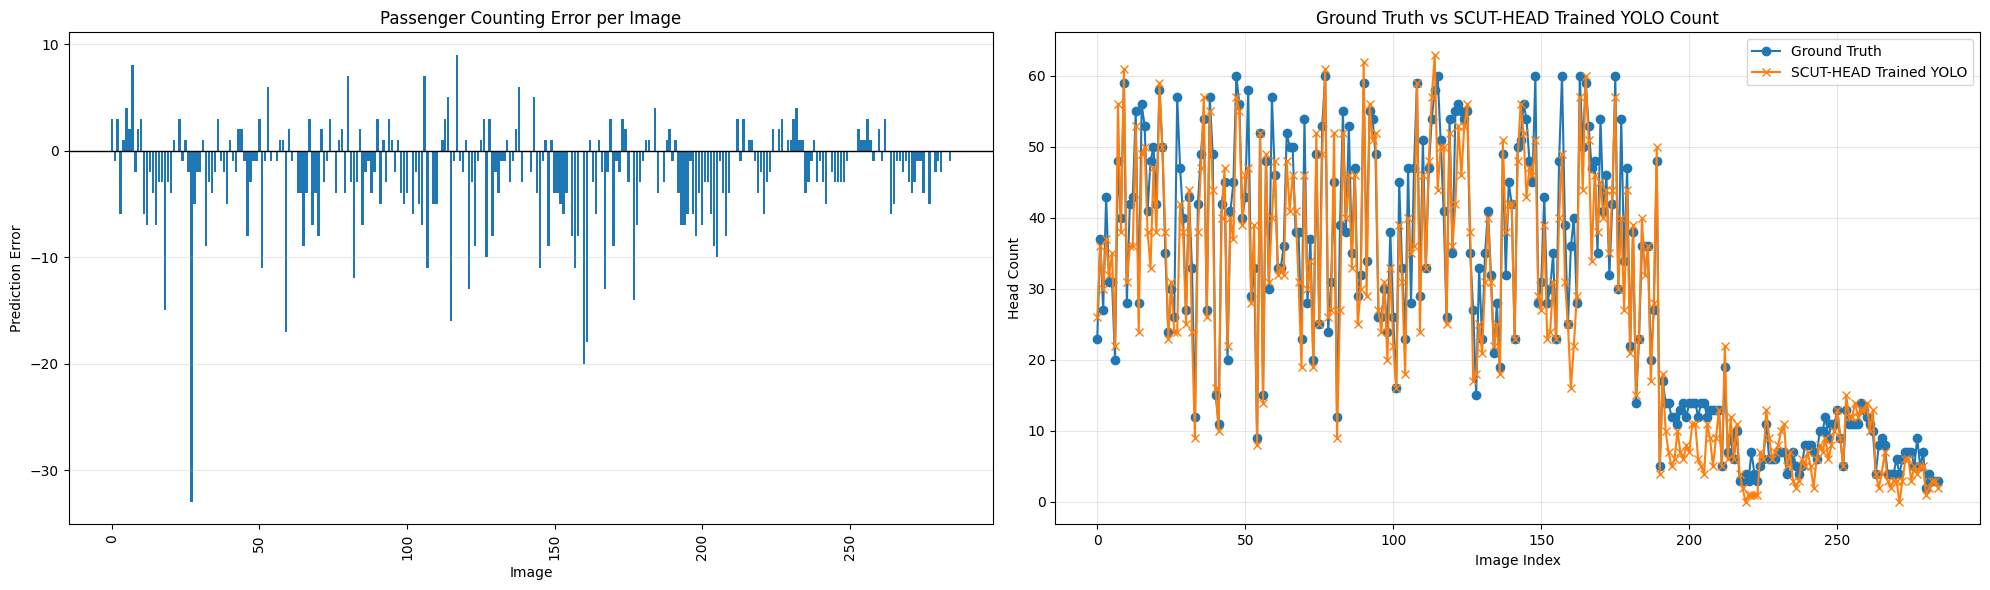
\includegraphics[width=1.0\linewidth]{./../images/sparse/scut_head_yolo/per_image_error_and_gt_vs_predicted.png}
	\caption{YOLO head detector counting error and predictions}
	\label{fig:scut_head_yolo_actual_predicted}
\end{figure}

The largest counting error occurred in a highly crowded image (ground truth of 57 heads, predicted 27, an error of $-30$), showing that occlusion remains a limitation even after fine tuning. This single image is an outlier: the next largest error is 15 heads, and it accounts for roughly 17\% of the total squared error, which is why the RMSE is noticeably larger than the MAE. The confusion matrix in Figure~\ref{fig:yolo_scuthead_confusion_matrix} further reflects the detector's remaining errors, while the wide variation in per image F1 scores indicates that detection performance depends strongly on scene density and occlusion conditions.

\begin{figure}[htbp]
	\centering
	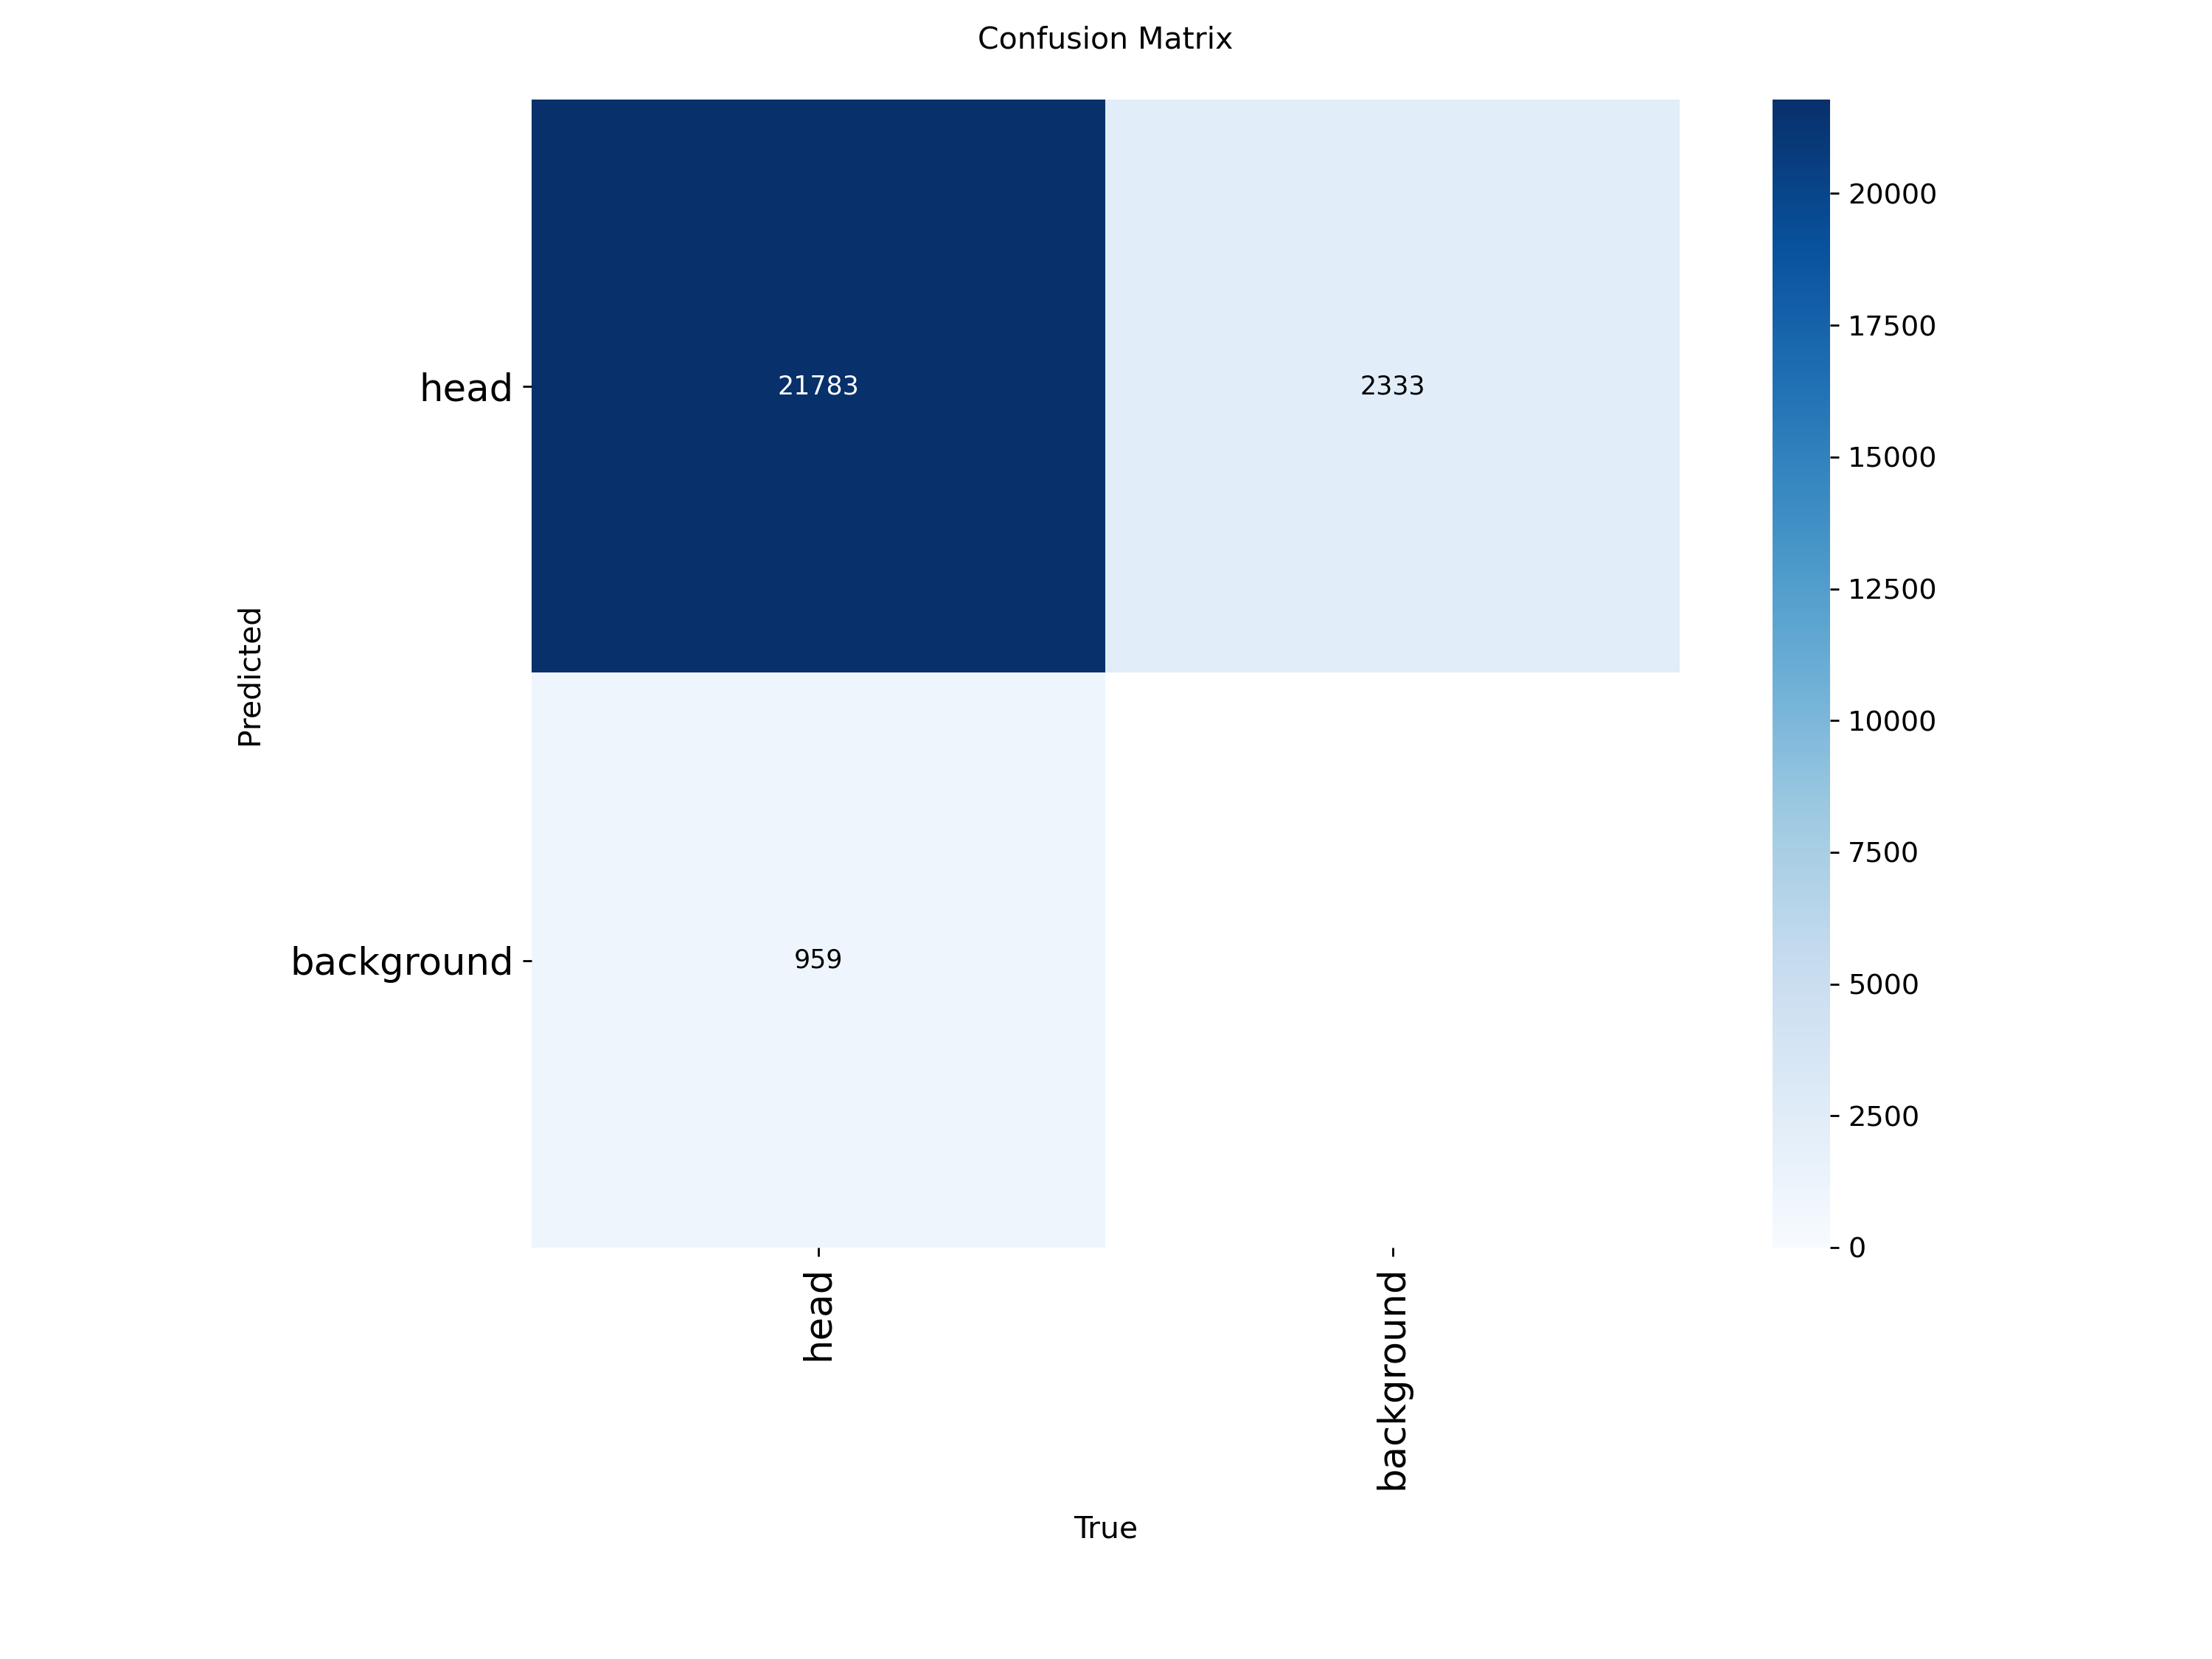
\includegraphics[width=0.7\linewidth]{./../images/sparse/scut_head_yolo/confusion_matrix.png}
	\caption{YOLO head detector confusion matrix}
	\label{fig:yolo_scuthead_confusion_matrix}
\end{figure}

\subsubsection{Performance by Ground Truth Count Range}

The results in Table~\ref{tab:scut_head_yolo_range_breakdown} and Figure~\ref{fig:scut_head_yolo_range_metrics} show that counting performance still depends on crowd density, but is substantially better than the pretrained detector. Absolute error generally increases with the number of people, from an MAE of 1.98 in the 1--10 range to 4.22 in the 51--60 range, although not strictly monotonically: the 21--30 range has the lowest MAE and RMSE, and the 11--20 range has a higher MAE than the 21--30 range. Relative error is highest in the sparsest scenes, where an error of one or two heads is a large fraction of a small count, and falls to roughly 7--9\% for scenes with more than 20 heads. Overall, counting accuracy remains relatively high and stable (about 91--93\%) across moderate to high density scenes.

\begin{figure}[htbp]
	\centering
	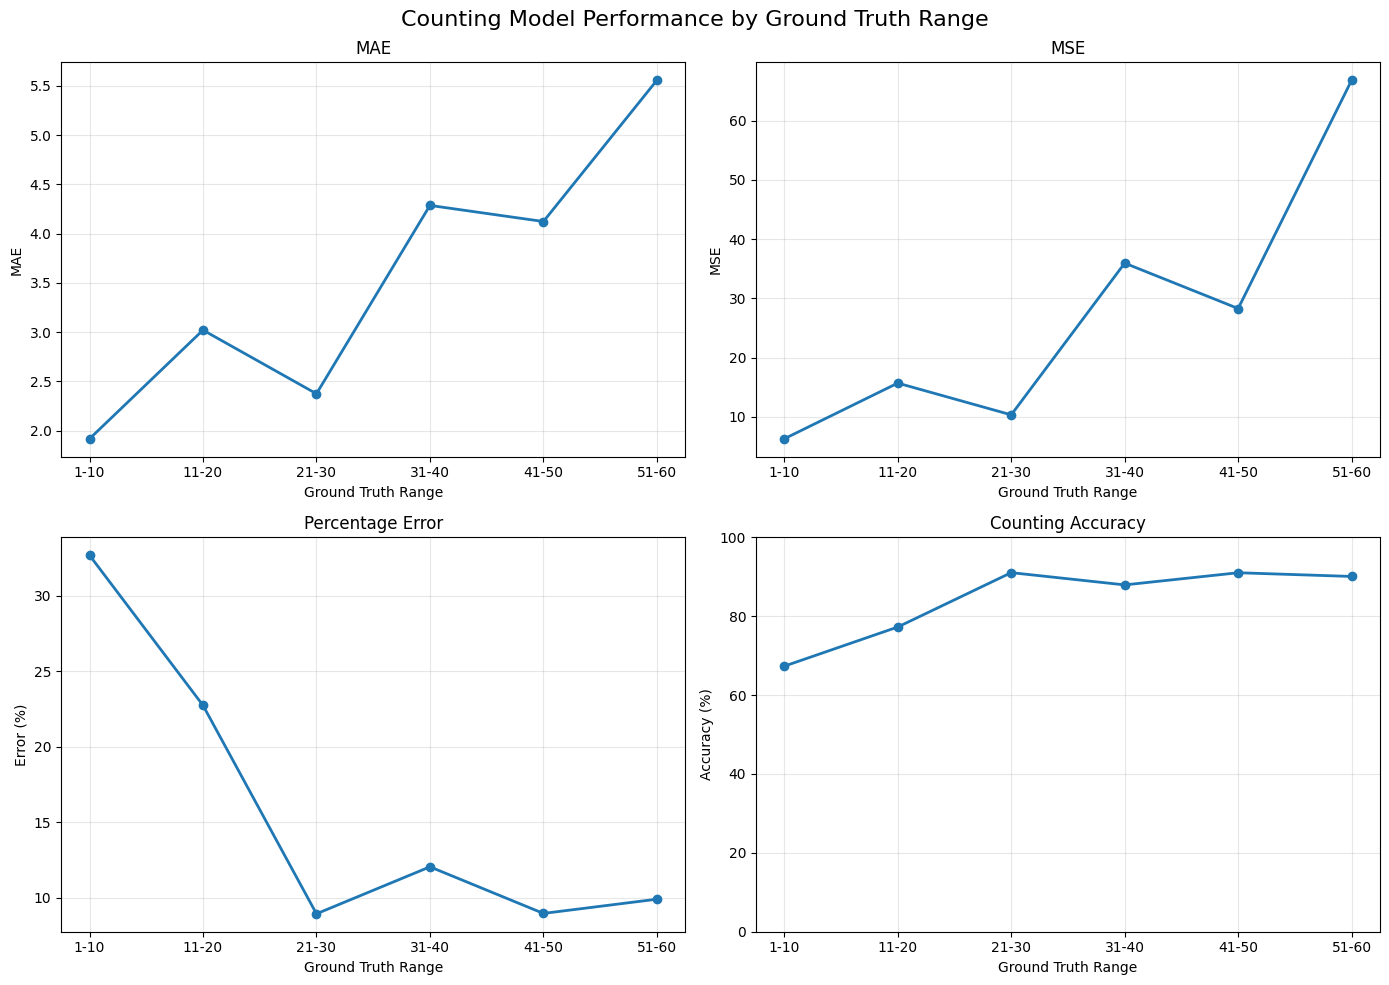
\includegraphics[width=1.0\linewidth]{./../images/sparse/scut_head_yolo/performance_by_gt_range.png}
	\caption{YOLO head detector performance across ground truth count ranges}
	\label{fig:scut_head_yolo_range_metrics}
\end{figure}

The counting bias remains negative across all density ranges and is largest in magnitude in the densest range (51--60 heads, a mean bias of $-2.89$), as shown in Table~\ref{tab:scut_head_yolo_range_breakdown}, although the increase with density is not strictly monotonic. This shows that fine tuning reduces but does not remove the undercounting caused by occlusion. Figure~\ref{fig:scut_head_yolo_range_metrics} further illustrates the decline in detection metrics as density increases: the mean F1 score falls steadily from 0.5015 in the 1--10 range to 0.3949 in the 51--60 range. When heads are heavily occluded, there is less visible information for the detector to identify them reliably.

\begin{longtable}{|
    >{\raggedright\arraybackslash}p{0.08\textwidth}|
    >{\centering\arraybackslash}p{0.04\textwidth}|
    >{\centering\arraybackslash}p{0.10\textwidth}|
    >{\centering\arraybackslash}p{0.10\textwidth}|
    >{\centering\arraybackslash}p{0.10\textwidth}|
    >{\centering\arraybackslash}p{0.14\textwidth}|
    >{\centering\arraybackslash}p{0.12\textwidth}|
    >{\centering\arraybackslash}p{0.10\textwidth}|
}

\caption{YOLO head detector performance breakdown by ground truth count range}
\label{tab:scut_head_yolo_range_breakdown} \\

\hline
\textbf{GT Range} &
\textbf{$n$} &
\textbf{MAE} &
\textbf{RMSE} &
\textbf{Mean \% Error} &
\textbf{Mean Acc. (\%)} &
\textbf{Mean Bias} &
\textbf{Mean F1} \\
\hline
\endfirsthead

\multicolumn{8}{|c|}%
{{\tablename\ \thetable{} -- continued from previous page}} \\
\hline
\textbf{GT Range} &
\textbf{$n$} &
\textbf{MAE} &
\textbf{RMSE} &
\textbf{Mean \% Error} &
\textbf{Mean Acc. (\%)} &
\textbf{Mean Bias} &
\textbf{Mean F1} \\
\hline
\endhead

\hline
\multicolumn{8}{|c|}{\textit{Continued on next page}} \\
\hline
\endfoot

\hline
\endlastfoot

1--10
& 61
& 1.9836
& 2.8716
& 34.1797
& 66.9913
& $-0.6066$
& \textbf{0.5015} \\
\hline

11--20
& 48
& 2.7292
& 3.4611
& 20.6059
& 79.3941
& $-1.2708$
& 0.4744 \\
\hline

21--30
& 40
& \textbf{1.9250}
& \textbf{2.5446}
& 7.2370
& 92.7630
& $-0.2250$
& 0.4611 \\
\hline

31--40
& 42
& 3.3571
& 5.0024
& 9.4020
& 90.5980
& $-1.4524$
& 0.4572 \\
\hline

41--50
& 49
& 3.1020
& 4.2857
& \textbf{6.8092}
& \textbf{93.1908}
& $-0.6122$
& 0.4259 \\
\hline

51--60
& 45
& 4.2222
& 6.4291
& 7.5245
& 92.4755
& $-2.8889$
& 0.3949 \\
\hline

\end{longtable}

Per-image counting accuracy is bounded below at 0\%, so Mean Acc.\ and Mean \% Error do not sum to 100\% in the 1--10 range, where one image (ground truth of 7 heads, predicted 19) has a percentage error above 100\%.

These results presented in Table~\ref{tab:scut_head_yolo_range_breakdown} and Figure~\ref{fig:scut_head_yolo_range_metrics} show that counting performance depends on crowd density. Percentage based counting accuracy is lowest in the sparsest scenes (66.99\% for 1--10 heads, where small denominators magnify errors) and stable at roughly 91--93\% from 21 heads upward, whereas absolute error, undercounting bias, and detection performance deteriorate in the densest scenes (51--60 heads: MAE of 4.22, mean bias of $-2.89$, mean F1 of 0.35). Compared with the pretrained detector, the fine tuned model has a more predictable failure pattern, but high density scenes remain challenging. This indicates that detection based counting has limitations that cannot be fully solved through additional training alone.

\subsection{FourColumn MCNN: Density Regression Network}
\label{sec:mcnn}

This section reports the experimental results obtained from training and evaluating the proposed MCNN density estimation model for crowd head counting. The model was trained to learn the relationship between input images and their corresponding density representations, with training and validation performance monitored using loss and mean absolute error (MAE). Although the training schedule was configured for a maximum of 100 epochs, the training process was terminated at epoch 98 as the validation performance had stabilised. The best performing checkpoint was obtained at epoch 68 based on the lowest validation loss and MAE. The results presented below examine the model's training behaviour, validation performance, and final evaluation results, providing an assessment of its effectiveness for density based crowd estimation.

\subsubsection{Training Performance and Convergence}

The training history covers 100 epochs and tracks training and validation loss and MAE, along with the best performing checkpoint. Both training and validation metrics improve substantially during the first $\sim$25 epochs, although validation performance is unstable early in training (for example, the validation MAE rises to 75.07 at epoch 7 before falling again). From approximately epoch 40 onward, all four metrics plateau and remain effectively constant until the final epoch. In contrast to the detection experiment in Section~\ref{sec:scut_yolo}, the MCNN does not employ a task specific pretrained backbone, requiring it to learn relevant features directly from the training data. The resulting progression of training and validation performance is presented in Figure~\ref{fig:mcnn_training_curves}.

\begin{figure}[htbp]
	\centering
	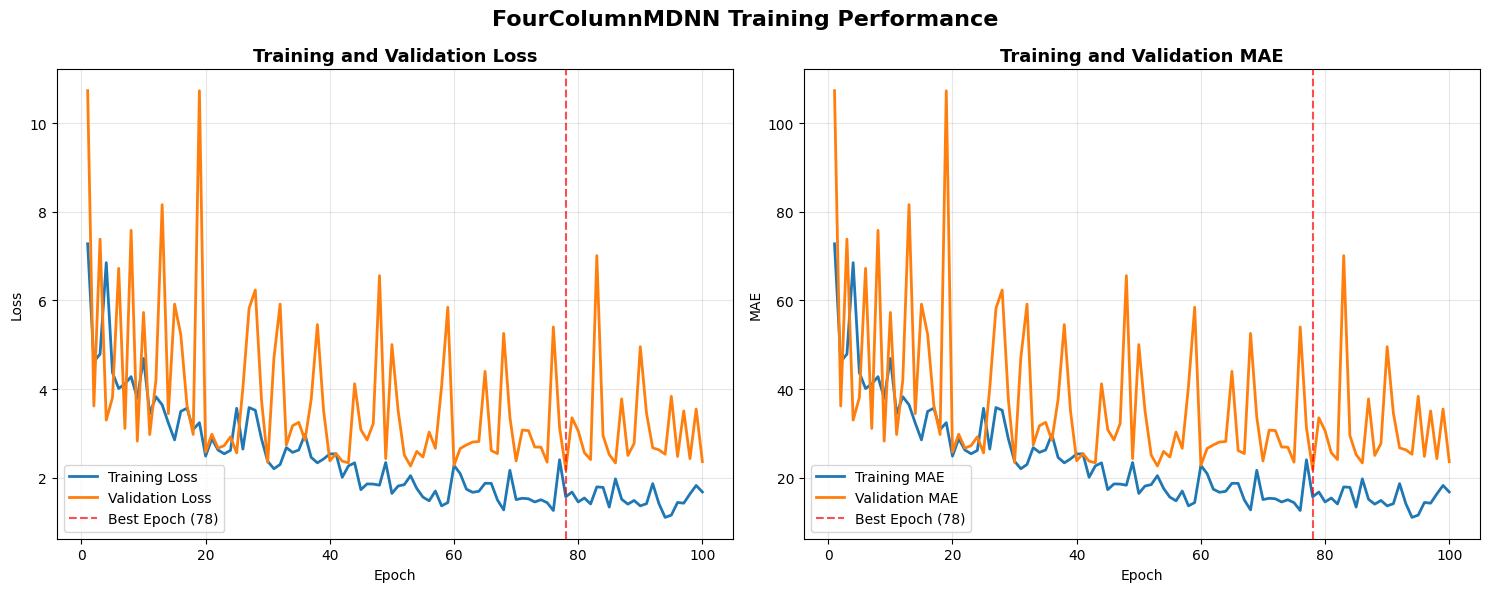
\includegraphics[width=1.0\linewidth]{./../images/dense/mcnn/training_validation_loss_mae_curves.png}
	\caption{FourColumn training and validation loss (left) and MAE (right).}
	\label{fig:mcnn_training_curves}
\end{figure}

The model achieves its best validation performance at epoch 68, with a validation loss of 2.3686 and MAE of 23.6775, as reported in Table~\ref{tab:mcnn_training_summary}. At this point the training and validation metrics are nearly identical (training MAE of 23.4910), so there is no evidence of overfitting or of a generalisation gap between the two sets. Instead, the values recorded from epoch 68 to the final epoch differ only at the fifth decimal place or beyond, meaning the selection of epoch 68 reflects negligible differences between plateaued epochs rather than a distinct optimum.

\begin{longtable}{|
>{\raggedright\arraybackslash}p{0.20\textwidth}|
>{\raggedright\arraybackslash}p{0.16\textwidth}|
>{\raggedright\arraybackslash}p{0.16\textwidth}|
>{\raggedright\arraybackslash}p{0.16\textwidth}|
>{\raggedright\arraybackslash}p{0.16\textwidth}|
}
\caption{FourColumn training progression summary at key epochs}
\label{tab:mcnn_training_summary} \\

\hline
\textbf{Epoch} &
\textbf{Train Loss} &
\textbf{Val Loss} &
\textbf{Train MAE} &
\textbf{Val MAE} \\
\hline
\endfirsthead

\multicolumn{5}{|c|}%
{{\tablename\ \thetable{} -- continued from previous page}} \\
\hline
\textbf{Epoch} &
\textbf{Train Loss} &
\textbf{Val Loss} &
\textbf{Train MAE} &
\textbf{Val MAE} \\
\hline
\endhead

\hline
\multicolumn{5}{|c|}{\textit{Continued on next page}} \\
\hline
\endfoot

\hline
\endlastfoot

1 (initial)
& 5.9387
& 10.1707
& 59.3778
& 101.7021 \\
\hline

68 (best validation)
& 2.3502
& \textbf{2.3686}
& 23.4910
& \textbf{23.6775} \\
\hline

98 (final)
& 2.3502
& 2.3687
& 23.4910
& 23.6775 \\
\hline

\end{longtable}

The flat training and validation curves beyond epoch 40, visible in Figure~\ref{fig:mcnn_training_curves} and reflected in the near identical key epoch values in Table~\ref{tab:mcnn_training_summary}, indicate that the model stopped improving well before the end of the training schedule. The training and validation errors converge to almost the same value, which suggests that the network settled into a fixed solution rather than continuing to refine its fit to the data. The checkpoint at epoch 68, corresponding to the minimum validation loss recorded in the training history, is therefore used for the evaluation below.

\subsubsection{Quantitative Density Based Counting Performance}

The aggregate results in Table~\ref{tab:mcnn_summary} are weaker than those of the YOLO based methods, reflecting the different error characteristics of density based estimation compared with object detection. The MCNN predicts continuous density maps rather than discrete objects, resulting in only modest correlation between predicted and ground truth counts and a negative coefficient of determination. These results suggest limited overall predictive reliability and are examined further through the density stratified analysis in the following subsection.

\begin{longtable}{|
>{\raggedright\arraybackslash}p{0.65\textwidth}|
>{\raggedright\arraybackslash}p{0.27\textwidth}|
}

\caption{MCNN counting performance}
\label{tab:mcnn_summary} \\

\hline
\textbf{Metric} & \textbf{Value} \\
\hline
\endfirsthead

\multicolumn{2}{|c|}{%
\textit{\tablename\ \thetable{} -- continued from previous page}} \\
\hline

\textbf{Metric} & \textbf{Value} \\
\hline
\endhead

\hline
\multicolumn{2}{|c|}{\textit{Continued on next page}} \\
\hline
\endfoot

\hline
\endlastfoot

Images
& 285 \\
\hline

Total Ground Truth
& 8{,}310 \\
\hline

Total Predicted
& 11{,}190.9073 \\
\hline

Mean Ground Truth Count
& 29.16 \\
\hline

Mean Predicted Count
& 39.2663 \\
\hline

Mean Bias (Predicted $-$ Ground Truth)
& 10.1084 \\
\hline

Mean Absolute Error (MAE)
& 14.7544 \\
\hline

Root Mean Squared Error (RMSE)
& 24.9473 \\
\hline

Mean Absolute Percentage Error (MAPE)
& 132.8992\% \\
\hline

\end{longtable}

The MCNN shows a systematic tendency toward overestimation, with the largest percentage errors occurring mainly in images with low ground truth counts. The aggregate statistics in Table~\ref{tab:mcnn_summary} show a mean predicted count of 39.2663 compared with a mean ground truth count of 29.16, and the model overestimates in 205 of the 285 test images. This pattern is evident in the per-image error distribution shown in Figure~\ref{fig:mcnn_actual_predicted}. A plausible explanation is the model's reliance on local texture and contextual cues rather than explicit object representations, which may cause background patterns or clutter to be interpreted as additional density. Such errors have a greater relative impact in sparse scenes than in densely populated ones.

\begin{figure}[htbp]
	\centering
	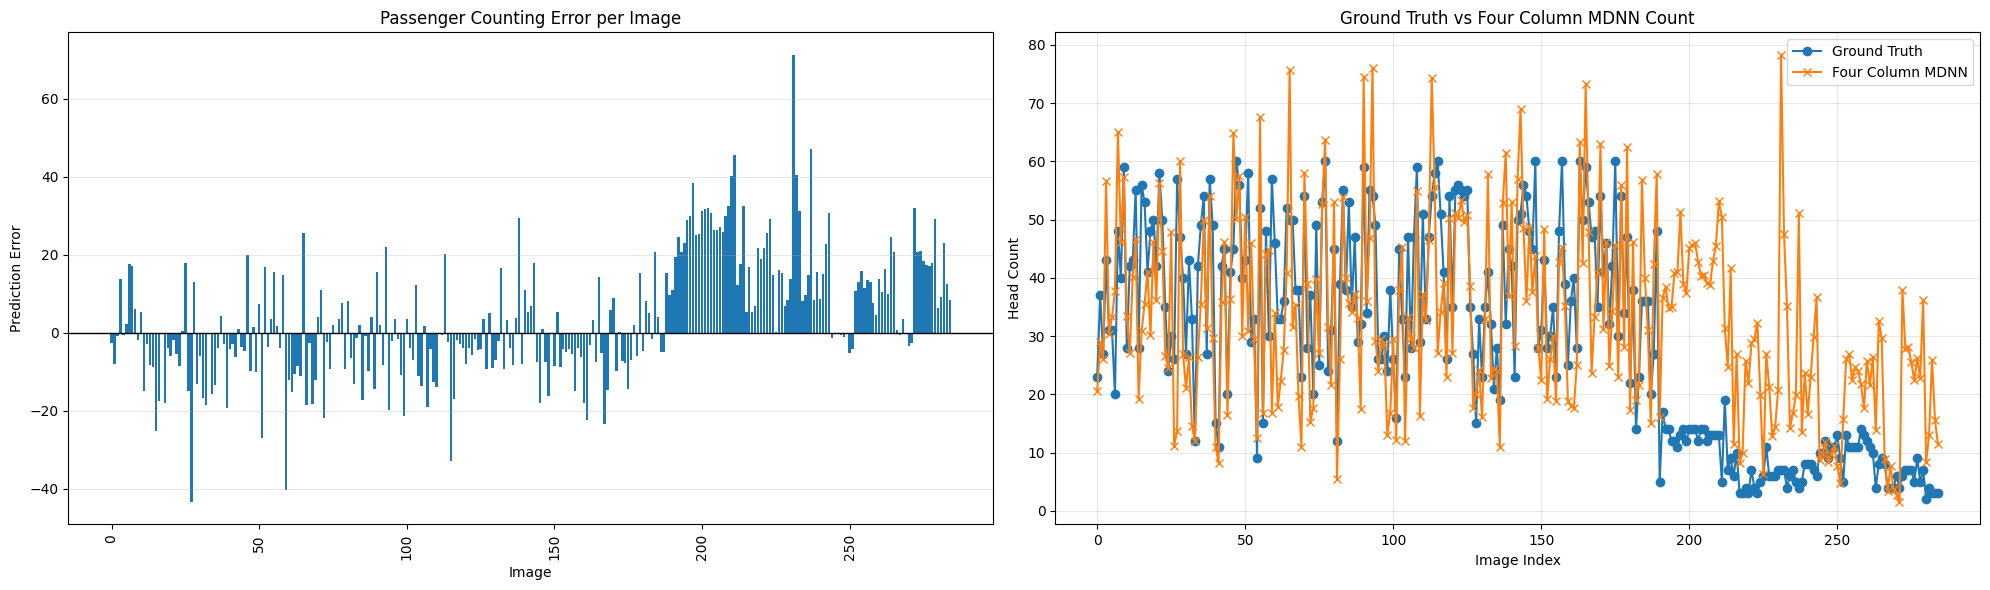
\includegraphics[width=1.0\linewidth]{./../images/dense/mcnn/per_image_error_and_gt_vs_predicted.png}
	\caption{MCNN counting error and predictions}
	\label{fig:mcnn_actual_predicted}
\end{figure}

A notable proportion of test images (55 of 285, or 19.3\%) have absolute errors equal to or greater than their ground truth counts, representing errors comparable to or worse than predicting zero. The most extreme cases are severe outliers: three sparse images with ground truth counts of 4, 7 and 7 receive predictions of approximately 124, 188 and 193, respectively. The per-image error plot in Figure~\ref{fig:mcnn_actual_predicted} illustrates the substantial variation in prediction error across the test set, while the aggregate error statistics in Table~\ref{tab:mcnn_summary} further quantify this variability.

\subsubsection{Performance by Ground Truth Count Range}

The density range results in Table~\ref{tab:mcnn_range_breakdown} and Figure~\ref{fig:mcnn_range_metrics} clarify the aggregate findings and reveal a pattern opposite to that of the detection based methods. While detection performance is strongest in sparse scenes and declines with increasing density, MCNN performs very poorly at the lowest counts (1--10), where the MAE is 26.400273 and the mean accuracy is only 12.394367\%. Performance then improves markedly from the 11--20 range onward, with the mean percentage error falling from 477.031561\% to 23.607820\% and the mean accuracy rising to 76.392180\% in the densest range, although these trends are not strictly monotonic between adjacent ranges. This behaviour is consistent with density regression, as stronger crowd density signals provide more reliable texture and contextual cues, whereas sparse scenes make background related noise more significant relative to the true count.

\begin{figure}[htbp]
	\centering
	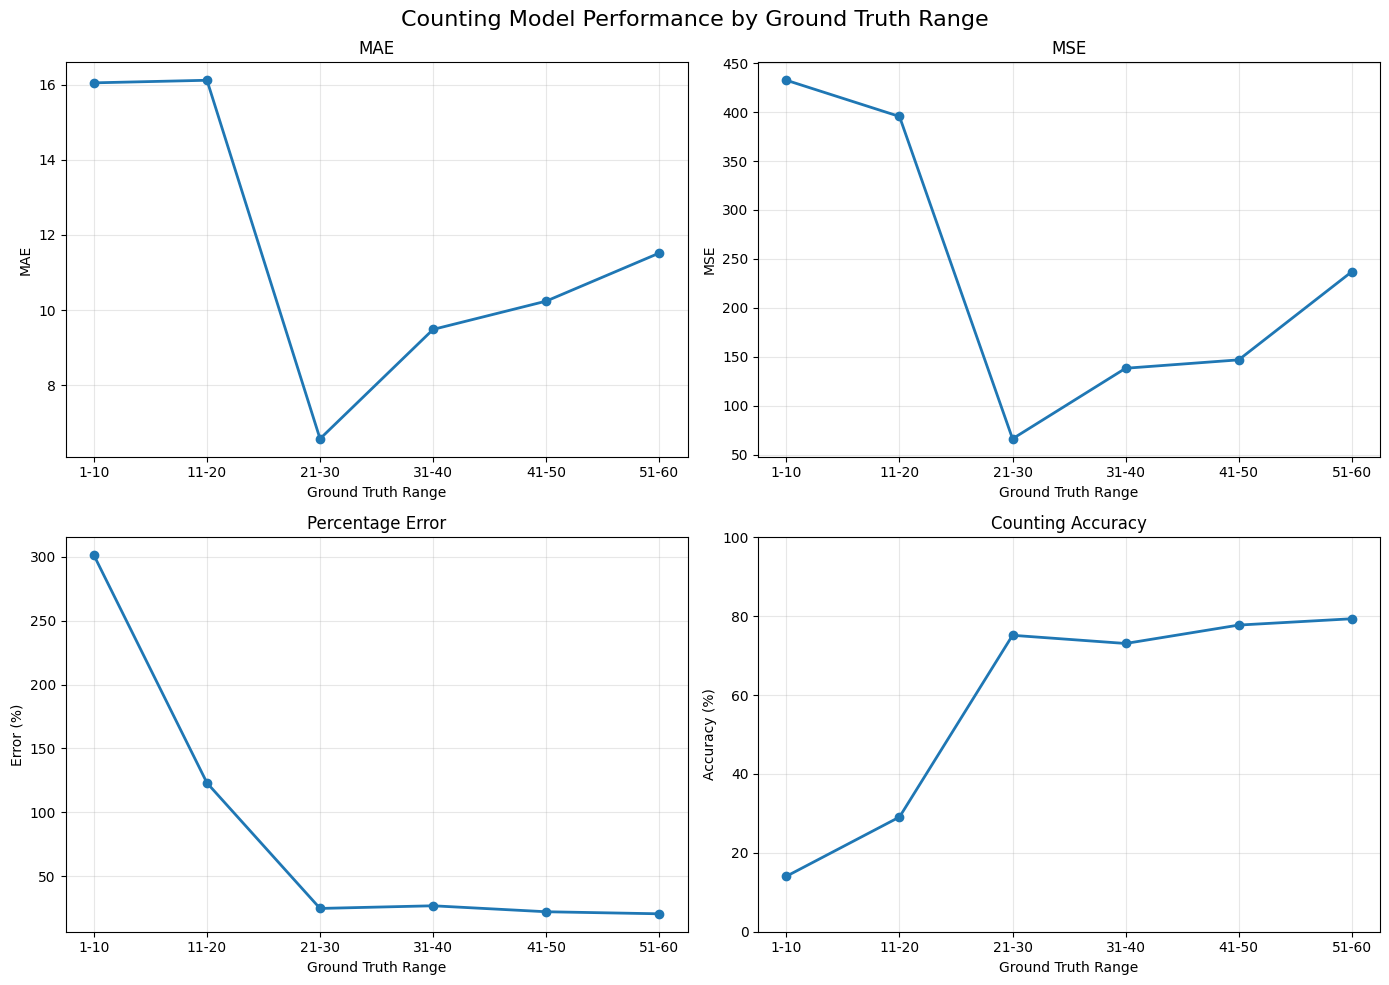
\includegraphics[width=1.0\linewidth]{./../images/dense/mcnn/performance_by_gt_range.png}
	\caption{MCNN performance across ground truth count ranges}
	\label{fig:mcnn_range_metrics}
\end{figure}

Absolute errors behave differently from relative errors. The lowest MAE (8.8044) and RMSE (13.5641) occur in the 11--20 range, after which absolute errors rise to roughly 10--14 counts in the higher ranges, as would be expected when the same relative error is applied to larger counts. The bias is positive in every range, indicating overestimation across all densities. It is strongest in the sparsest scenes (+25.7247 for counts of 1--10), where overestimation is likely driven by background and textural noise, and decreases steadily as density increases, reaching +3.8367 in the 51--60 range. Unlike a model that underestimates dense crowds, the MCNN therefore shows no sign of a sign reversal in bias at higher densities within the count range tested.

\begin{longtable}{|
    >{\raggedright\arraybackslash}p{0.12\textwidth}|
    >{\centering\arraybackslash}p{0.04\textwidth}|
    >{\centering\arraybackslash}p{0.10\textwidth}|
    >{\centering\arraybackslash}p{0.10\textwidth}|
    >{\centering\arraybackslash}p{0.10\textwidth}|
    >{\centering\arraybackslash}p{0.18\textwidth}|
    >{\centering\arraybackslash}p{0.14\textwidth}|
    >{\centering\arraybackslash}p{0.10\textwidth}|
}

\caption{MCNN performance breakdown by ground truth count range}
\label{tab:mcnn_range_breakdown} \\

\hline
\textbf{GT Range} &
\textbf{$n$} &
\textbf{MAE} &
\textbf{RMSE} &
\textbf{Mean \% Error} &
\textbf{Mean Accuracy (\%)} &
\textbf{Mean Bias} \\
\hline
\endfirsthead

\multicolumn{7}{|c|}%
{{\tablename\ \thetable{} -- continued from previous page}} \\
\hline
\textbf{GT Range} &
\textbf{$n$} &
\textbf{MAE} &
\textbf{RMSE} &
\textbf{Mean \% Error} &
\textbf{Mean Accuracy (\%)} &
\textbf{Mean Bias} \\
\hline
\endhead

\hline
\multicolumn{7}{|c|}{\textit{Continued on next page}} \\
\hline
\endfoot

\hline
\endlastfoot

1--10
& 61
& 26.4003
& 45.0173
& 477.0316
& 12.3944
& 25.7247 \\
\hline

11--20
& 48
& \textbf{8.8044}
& \textbf{13.5641}
& 66.6543
& 50.0811
& 7.9943 \\
\hline

21--30
& 40
& 9.8021
& 14.6656
& 38.4039
& 66.5747
& 5.7950 \\
\hline

31--40
& 42
& 13.9458
& 17.3380
& 39.5928
& 61.4024
& 5.6436 \\
\hline

41--50
& 49
& 12.2487
& 15.1478
& 26.8679
& 73.1321
& 5.8468 \\
\hline

51--60
& 45
& 13.1995
& 16.6341
& \textbf{23.6078}
& \textbf{76.3922}
& \textbf{3.8367} \\
\hline

\end{longtable}

Taken together with the range based results of the two detection based methods, these findings provide empirical support for combining detection and density based counting in a single adaptive framework. MCNN performs least reliably in sparse scenes, where detection based methods are strongest, while its relative accuracy improves at higher densities, where detection methods are increasingly affected by occlusion. Thus, the two approaches exhibit complementary strengths across different crowd density conditions rather than differing solely in overall accuracy.

\subsection{CSRNet: VGG-16 Based Density Regression Network}
\label{sec:csrnet}

This section reports the experimental results obtained from training and evaluating CSRNet for crowd head counting on the same 285-image test set used throughout this chapter. Similar to the proposed MCNN described in Section~\ref{sec:mcnn}, CSRNet estimates a continuous density map and derives the final crowd count by integrating the predicted density rather than explicitly localising individual heads. The two networks therefore represent alternative implementations of the density based counting paradigm and can be compared directly in terms of their training behaviour, aggregate counting accuracy, and performance across different crowd-density ranges.

\subsubsection{Training Performance and Convergence}

The CSRNet training history covers up to 100 epochs and records training and validation loss together with the corresponding MAE values. As illustrated in Figure~\ref{fig:csrnet_training_curves}, both training and validation loss decrease sharply during the first few epochs, falling by several orders of magnitude from their initial values, and then converge gradually as training progresses. The best validation performance is reached at epoch 35. With an early stopping patience of 30 epochs, training was automatically terminated at epoch 65 because no further improvement in the validation performance was observed after the best epoch. Consequently, although the maximum training schedule was set to 100 epochs, the model completed training at epoch 65, indicating that the validation performance had largely stabilised before the final epoch.

\begin{figure}[htbp]
	\centering
	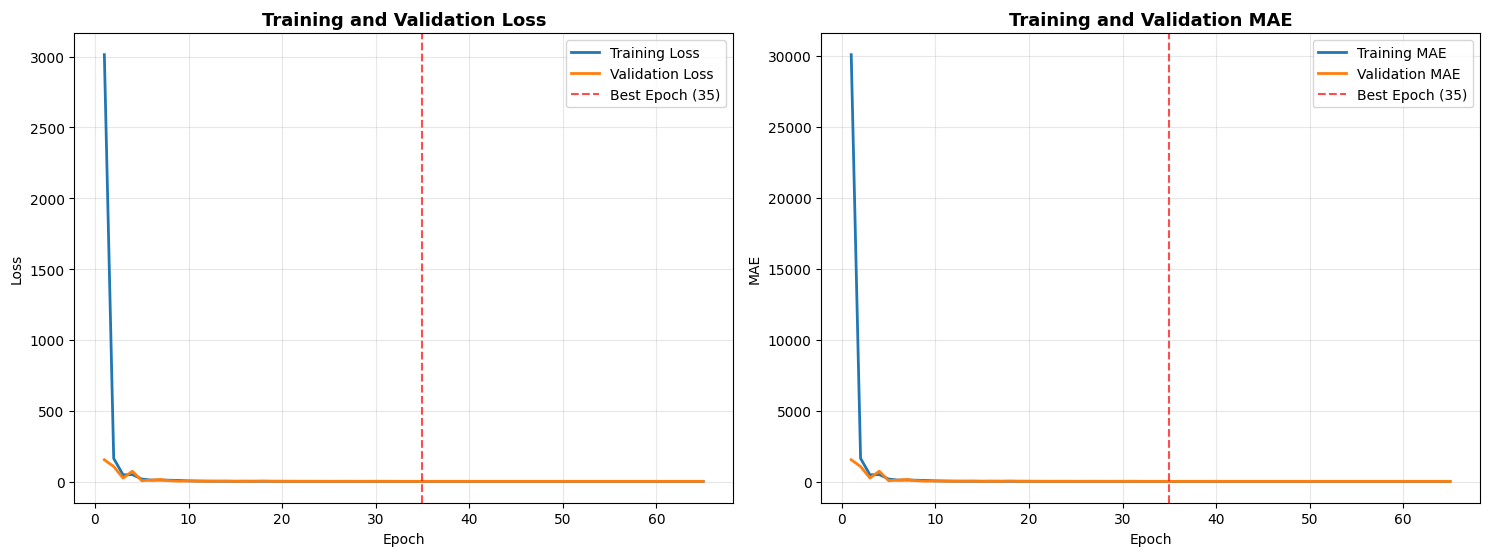
\includegraphics[width=1.0\linewidth]{./../images/dense/csrnet/training_validation_loss_mae_curves.png}
	\caption{CSRNet training and validation loss (left) and MAE (right).}
	\label{fig:csrnet_training_curves}
\end{figure}

Figure~\ref{fig:csrnet_training_curves} shows that CSRNet converges substantially during the early epochs, followed by a gradual reduction in both training and validation error. CSRNet exhibits no comparable post-optimal divergence: after epoch 35 the validation loss increases only marginally, from 1.4370 to 1.4455 at the final epoch, while the training loss decreases only slightly over the same interval. The key training values are summarised in Table~\ref{tab:csrnet_training_summary}.

\begin{longtable}{|
>{\raggedright\arraybackslash}p{0.20\textwidth}|
>{\raggedright\arraybackslash}p{0.16\textwidth}|
>{\raggedright\arraybackslash}p{0.16\textwidth}|
>{\raggedright\arraybackslash}p{0.16\textwidth}|
>{\raggedright\arraybackslash}p{0.16\textwidth}|
}
\caption{CSRNet training progression summary at key epochs}
\label{tab:csrnet_training_summary} \\

\hline
\textbf{Epoch} &
\textbf{Train Loss} &
\textbf{Val Loss} &
\textbf{Train MAE} &
\textbf{Val MAE} \\
\hline
\endfirsthead

\multicolumn{5}{|c|}%
{{\tablename\ \thetable{} -- continued from previous page}} \\
\hline
\textbf{Epoch} &
\textbf{Train Loss} &
\textbf{Val Loss} &
\textbf{Train MAE} &
\textbf{Val MAE} \\
\hline
\endhead

\hline
\multicolumn{5}{|c|}{\textit{Continued on next page}} \\
\hline
\endfoot

\hline
\endlastfoot

1 (initial)
& 3013.3745
& 153.6462
& 30077.7497
& 1535.9628 \\
\hline

35 (best validation)
& 1.1113
& \textbf{1.4370}
& 11.1055
& \textbf{14.3642} \\
\hline

65 (final)
& \textbf{1.0916}
& 1.4455
& \textbf{10.9087}
& 14.4489 \\
\hline

\end{longtable}

The final training and validation metrics remain closely aligned in relative terms, with a residual train/validation MAE gap of approximately 3.54 that is established by around epoch 40 and remains effectively constant thereafter, as indicated by Figure~\ref{fig:csrnet_training_curves}. This behaviour suggests that CSRNet does not exhibit the same degree of post-optimal training divergence observed for MCNN. Instead, the model reaches a stable solution in which further reductions in training error produce little change in validation performance. The loss and MAE values reported here are associated with normalised or rescaled density targets rather than raw head counts, and should therefore be interpreted primarily as indicators of optimisation behaviour rather than as direct measures of the image level counting error reported in Table~\ref{tab:csrnet_training_summary}.

Compared with MCNN, CSRNet therefore demonstrates a more stable training trajectory. MCNN continues to reduce its training error after its best validation checkpoint at epoch 80, whereas CSRNet's training and validation metrics remain closely coupled toward the end of training and plateau together. This indicates that CSRNet achieves a comparatively stable convergence pattern, although the stability of the training process does not by itself imply high counting accuracy on unseen test images.

\subsubsection{Quantitative Density Based Counting Performance}

The aggregate CSRNet results are presented in Table~\ref{tab:csrnet_training_summary}. Compared with the MCNN results in Table~\ref{tab:mcnn_summary}, CSRNet achieves lower MAE and RMSE. These results indicate that CSRNet provides an overall improvement in count prediction relative to MCNN. However, the correlation remains moderate and the relative errors remain substantial, with a MAPE in excess of 100\%, showing that the improvement does not translate into consistently accurate predictions across the complete test set.

\begin{longtable}{|
>{\raggedright\arraybackslash}p{0.65\textwidth}|
>{\raggedright\arraybackslash}p{0.27\textwidth}|
}

\caption{MCNN counting performance}
\label{tab:csrnet_summary} \\

\hline
\textbf{Metric} & \textbf{Value} \\
\hline
\endfirsthead

\multicolumn{2}{|c|}%
{{\tablename\ \thetable{} -- continued from previous page}} \\
\hline
\textbf{Metric} & \textbf{Value} \\
\hline
\endhead

\hline
\multicolumn{2}{|c|}{\textit{Continued on next page}} \\
\hline
\endfoot

\hline
\endlastfoot

Images
& 285 \\
\hline

Total Ground Truth
& 8{,}310 \\
\hline

Total Predicted
& 10{,}197.7373 \\
\hline

Mean Ground Truth Count
& 29.16 \\
\hline

Mean Predicted Count
& 35.78 \\
\hline

Mean Absolute Error (MAE)
& 10.8765 \\
\hline

Root Mean Squared Error (RMSE)
& 16.2645 \\
\hline

Mean Absolute Percentage Error (MAPE)
& 101.7975\% \\
\hline

\end{longtable}

The per-image prediction behaviour is illustrated in Figure~\ref{fig:csrnet_actual_predicted}, which shows the counting error for individual test images together with the relationship between ground truth and predicted counts. The figure demonstrates that, despite the improvement in aggregate metrics, substantial variation remains between individual predictions.

\begin{figure}[htbp]
	\centering
	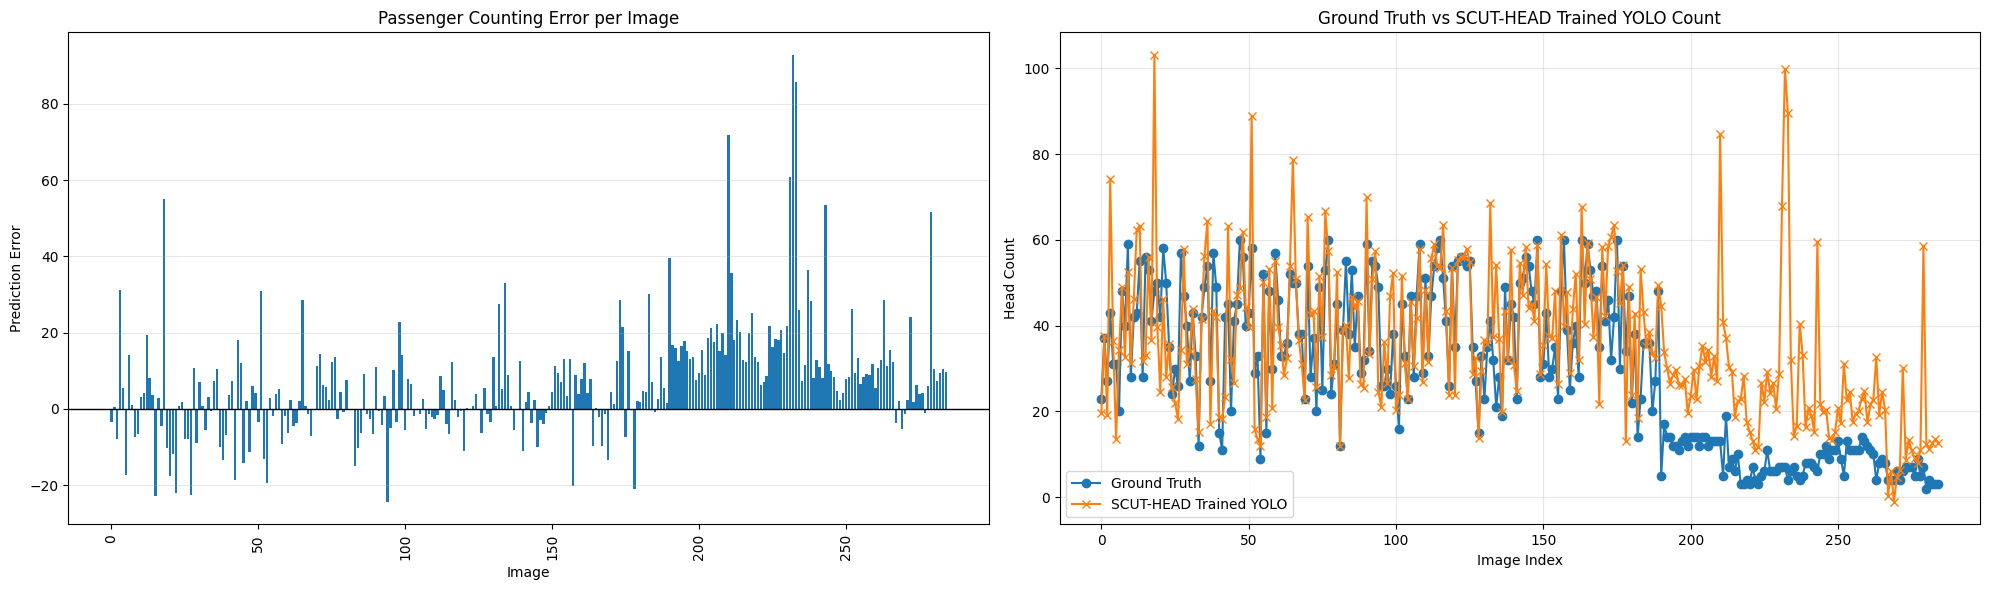
\includegraphics[width=1.0\linewidth]{./../images/dense/csrnet/per_image_error_and_gt_vs_predicted.png}
	\caption{CSRNet counting error and predictions }
	\label{fig:csrnet_actual_predicted}
\end{figure}

As shown in Figure~\ref{fig:csrnet_actual_predicted}, CSRNet exhibits a pronounced systematic tendency toward overestimation, with the mean predicted count of 35.78 exceeding the mean ground truth count of 29.16 by approximately 6.62 individuals, as reported in Table~\ref{tab:csrnet_training_summary}. Overestimation is the dominant error direction, affecting 196 of the 285 test images (68.8\%). The most extreme errors are all associated with sparse scenes: the model overestimates a ground truth count of 7 by 92.91 individuals, a ground truth count of 4 by 85.66 individuals, and a ground truth count of 13 by 71.76 individuals. Furthermore, 66 of the 285 test images (23.2\%) have an absolute error at least as large as the corresponding ground truth count. This indicates that, despite its improved aggregate performance over MCNN, CSRNet retains a substantial vulnerability to large counting errors in sparse scenes.

\subsubsection{Performance by Ground Truth Count Range}

To examine whether the aggregate improvement of CSRNet is consistent across different crowd densities, its performance is evaluated using the same ground truth count ranges applied to MCNN. Table~\ref{tab:csrnet_range_breakdown} and Figure~\ref{fig:csrnet_range_metrics} show the resulting density stratified performance.

\begin{figure}[htbp]
	\centering
	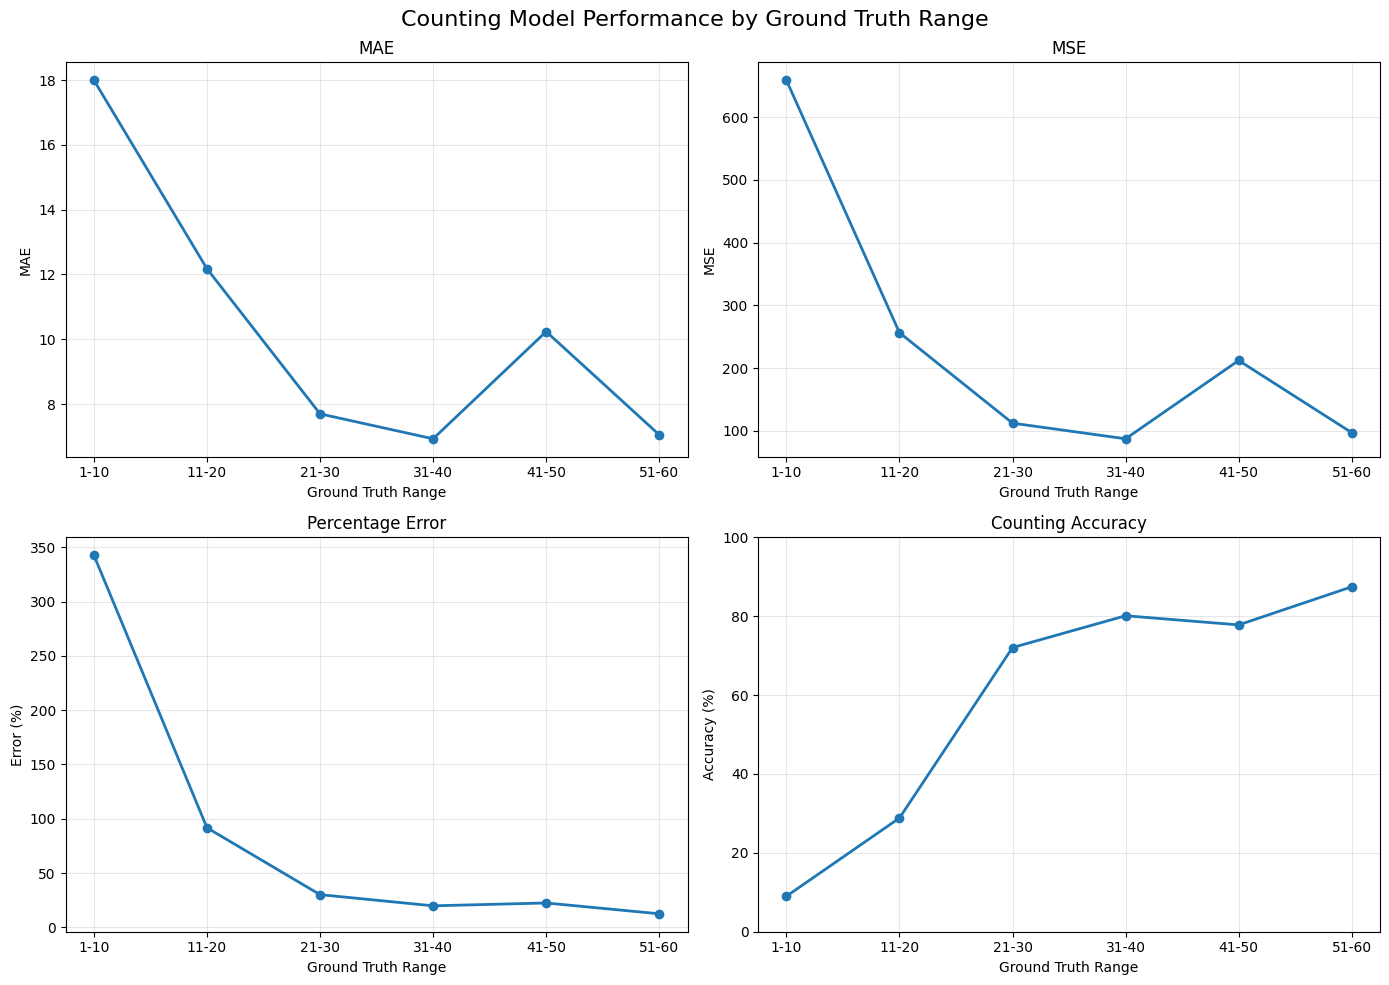
\includegraphics[width=1.0\linewidth]{./../images/dense/csrnet/performance_by_gt_range.png}
	\caption{CSRNet performance across ground truth count ranges}
	\label{fig:csrnet_range_metrics}
\end{figure}

Figure~\ref{fig:csrnet_range_metrics} shows a clear dependence of CSRNet performance on ground truth crowd density. The largest errors occur in the sparsest range of 1--10 individuals, where the MAE of 17.9970 exceeds the upper bound of the range itself and the mean counting accuracy falls to 9.0027\%. The error decreases substantially in the moderate density ranges and reaches its minimum in the 31--40 range, after which performance remains comparatively strong at higher counts, with the 51--60 range achieving the highest mean accuracy of 87.4577\%. This pattern is broadly consistent with the behaviour observed for MCNN in Figure~\ref{fig:mcnn_range_metrics}, although CSRNet generally achieves lower errors in the moderate and high density regimes.

\begin{longtable}{|
    >{\raggedright\arraybackslash}p{0.14\textwidth}|
    >{\centering\arraybackslash}p{0.04\textwidth}|
    >{\centering\arraybackslash}p{0.10\textwidth}|
    >{\centering\arraybackslash}p{0.10\textwidth}|
    >{\centering\arraybackslash}p{0.10\textwidth}|
    >{\centering\arraybackslash}p{0.16\textwidth}|
    >{\centering\arraybackslash}p{0.16\textwidth}|
}

\caption{CSRNet performance breakdown by ground truth count range}
\label{tab:csrnet_range_breakdown} \\

\hline
\textbf{GT Range} & \textbf{$n$} & \textbf{MAE} & \textbf{RMSE} &
\textbf{Mean \% Error} & \textbf{Mean Accuracy (\%)} & \textbf{Mean Bias} \\
\hline
\endfirsthead

\hline
\textbf{GT Range} & \textbf{$n$} & \textbf{MAE} & \textbf{RMSE} &
\textbf{Mean \% Error} & \textbf{Mean Accuracy (\%)} & \textbf{Mean Bias} \\
\hline
\endhead

\hline
\multicolumn{7}{|r|}{\textit{Continued on next page}} \\
\hline
\endfoot

\hline
\endlastfoot

1--10
& 61
& 17.9970
& 25.6650
& 342.6321
& 9.0027
& 17.6322 \\
\hline

11--20
& 48
& 12.1761
& 16.0101
& 91.7234
& 28.8339
& 12.1203 \\
\hline

21--30
& 40
& 7.6959
& 10.5910
& 30.1654
& 72.0535
& 3.6635 \\
\hline

31--40
& 42
& \textbf{6.9258}
& \textbf{9.3402}
& 19.8847
& 80.1153
& $-0.3179$ \\
\hline

41--50
& 49
& 10.2369
& 14.5630
& 22.5070
& 77.7984
& 2.8602 \\
\hline

51--60
& 45
& 7.0492
& 9.8493
& \textbf{12.5423}
& \textbf{87.4577}
& $-0.9542$ \\

\end{longtable}

The mean bias values reveal the underlying mechanism of this density dependence. In the two sparsest ranges the bias is large and strongly positive, at $+17.6322$ and $+12.1203$ respectively, indicating that CSRNet consistently hallucinates density in scenes containing few individuals. The bias diminishes markedly from the 21--30 range onward and approaches zero in the densest ranges, at $-0.3179$ for 31--40 and $-0.9542$ for 51--60. The residual aggregate overestimation reported in Table~\ref{tab:csrnet_training_summary} is therefore driven almost entirely by the sparse scene images rather than by a uniform offset across the test set.

The density stratified results therefore show that CSRNet improves upon MCNN primarily when a sufficient density signal is present. At low counts, neither density regression architecture provides the reliability achieved by the detection based methods. This supports the density adaptive interpretation: detection based counting is better suited to sparse scenes, while density based methods become more competitive as crowd density increases and individual localisation becomes more difficult.

\subsection{Hybrid Adaptive Counting: SCUT-Head YOLO Combined with MCNN}
\label{sec:hybrid_mcnn}

The previous sections show that the SCUT-Head YOLO detector and density regression networks have complementary strengths on the 285-image test set. The fine tunedCUT-Head YOLO detector (Section~\ref{sec:scut_yolo}) performs well in sparse and moderately crowded scenes but increasingly undercounts as crowd density and occlusion increase. In contrast, the density regression networks (Sections~\ref{sec:mcnn} and~\ref{sec:csrnet}) are less reliable in sparse scenes due to background noise but become more stable in dense crowds. This section presents a hybrid counting framework that combines the per-image predictions of the SCUT-Head YOLO detector and the MCNN density estimator to benefit from their complementary strengths, using the same 285-image test set.

\subsubsection{Quantitative Performance Evaluation}

Table~\ref{tab:hybrid_mcnn_summary} reports the aggregate counting performance of the hybrid framework on the 285-image test set. The total and mean ground truth counts match those reported for the individual detection and density based models in the preceding sections, confirming that the same test set is used throughout.

\begin{longtable}{|
>{\raggedright\arraybackslash}p{0.65\textwidth}|
>{\raggedright\arraybackslash}p{0.27\textwidth}|
}
\caption{Hybrid YOLO+MCNN counting performance}
\label{tab:hybrid_mcnn_summary} \\
\hline
\textbf{Metric} & \textbf{Value} \\
\hline
\endfirsthead

\multicolumn{2}{|c|}%
{{\tablename\ \thetable{} -- continued from previous page}} \\
\hline
\textbf{Metric} & \textbf{Value} \\
\hline
\endhead

\hline
\multicolumn{2}{|r|}{{Continued on next page}} \\
\hline
\endfoot

\hline
\endlastfoot

Images & 285 \\
\hline
Total Ground Truth & 8{,}310 \\
\hline
Total Predicted & 8{,}433.34 \\
\hline
Mean Ground Truth Count & 29.16 \\
\hline
Mean Predicted Count & 29.5907 \\
\hline
Mean Absolute Error (MAE) & 3.9813 \\
\hline
Root Mean Squared Error (RMSE) & 5.7401 \\
\hline
Mean Absolute Percentage Error (MAPE) & 21.7678\% \\
\hline

\end{longtable}

To determine whether adaptive fusion is beneficial relative to either constituent model in isolation, Table~\ref{tab:hybrid_mcnn_component_comparison} compares the hybrid framework directly against the SCUT-Head YOLO detector and the MCNN density estimator evaluated independently on the same 285 images.

\begin{figure}[htbp]
	\centering
	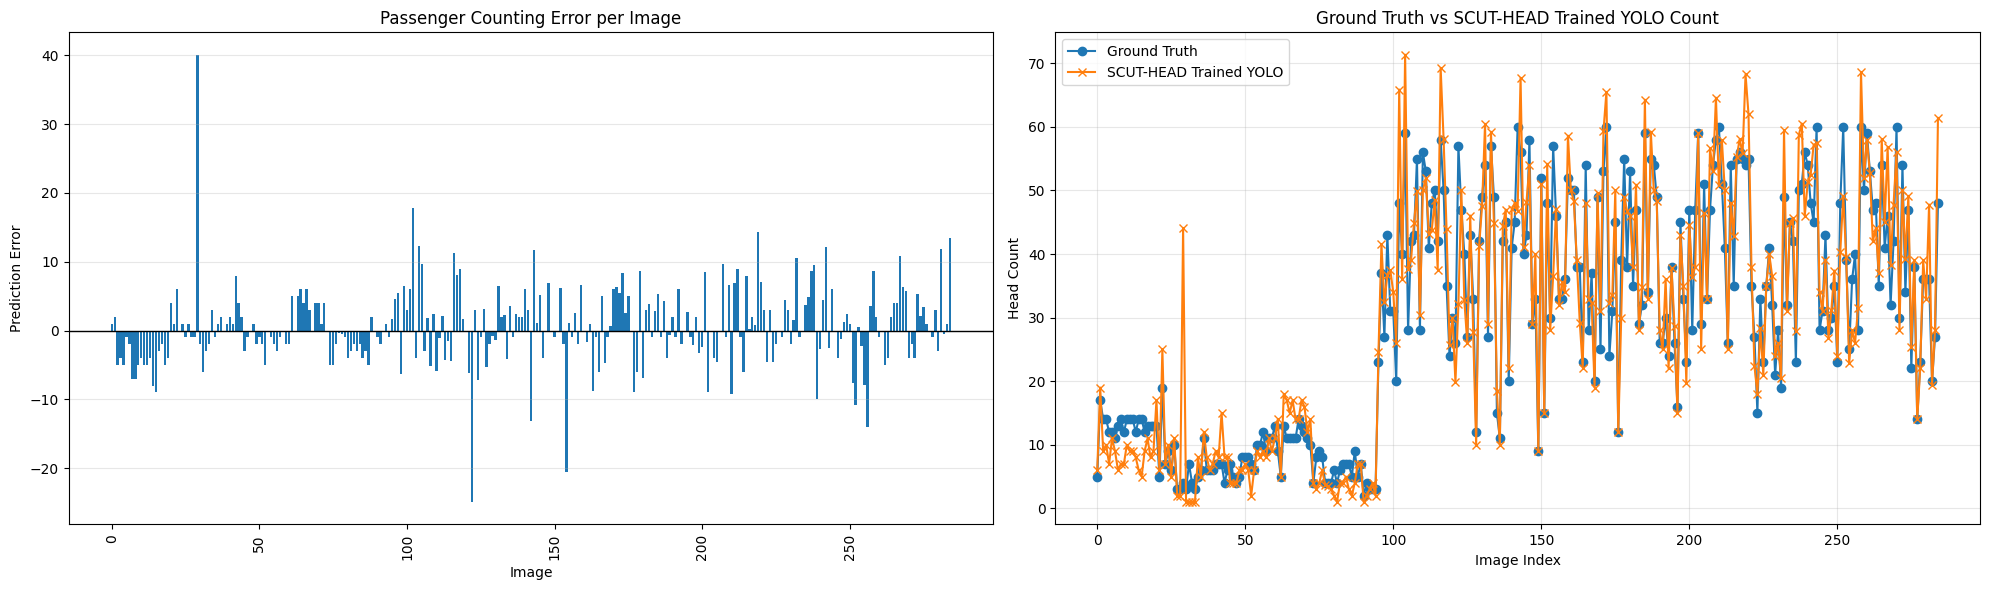
\includegraphics[width=1.0\linewidth]{./../images/scut_head_mcnn/per_image_error_and_gt_vs_predicted.png}
	\caption{Hybrid YOLO+MCNN counting error and predictions.}
	\label{fig:hybrid_actual_predicted}
\end{figure}

\begin{longtable}{|>{\raggedright\arraybackslash}p{7.0cm}|
                    >{\centering\arraybackslash}p{2.3cm}|
                    >{\centering\arraybackslash}p{2.3cm}|
                    >{\centering\arraybackslash}p{2.3cm}|}
\caption{Comparison of hybrid YOLO+MCNN and constituent models.}
\label{tab:hybrid_mcnn_component_comparison} \\
\hline
\textbf{Model} & \textbf{MAE} & \textbf{RMSE} & \textbf{MAPE (\%)} \\
\hline
\endfirsthead

\multicolumn{4}{|c|}%
{\tablename\ \thetable{} -- continued from previous page} \\
\hline
\textbf{Model} & \textbf{MAE} & \textbf{RMSE} & \textbf{MAPE (\%)} \\
\hline
\endhead

\hline
\multicolumn{4}{|c|}{Continued on next page} \\
\hline
\endfoot

\hline
\endlastfoot

SCUT-Head YOLO (detector only)
& \textbf{2.8491}
& \textbf{4.2501}
& \textbf{15.55} \\
\hline

MCNN (density only)
& 14.7544
& 24.9473
& 132.8992 \\
\hline

Hybrid (adaptive fusion)
& 3.9813
& 5.7401
& 21.7678 \\
\hline

\end{longtable}

However, Table~\ref{tab:hybrid_mcnn_component_comparison} shows that the hybrid framework does not outperform the SCUT-Head YOLO detector. YOLO achieves lower MAE, RMSE, and MAPE. This indicates that YOLO is already a strong counting method on this test set, while adding the noisier MCNN predictions introduces some additional error. Therefore, as further reflected in Figure~\ref{fig:hybrid_actual_predicted}, the main advantage of the hybrid framework is not better overall performance than YOLO, but providing a more reliable alternative to MCNN alone, particularly across different crowd-density and count ranges.

\subsubsection{Performance by Density Category}

Table~\ref{tab:hybrid_density_breakdown} reports hybrid counting performance stratified by the sparse/dense scene labels used to condition the fusion rule.

\begin{longtable}{|>{\raggedright\arraybackslash}p{1.5cm}|
                    >{\centering\arraybackslash}p{1.0cm}|
                    >{\centering\arraybackslash}p{1.2cm}|
                    >{\centering\arraybackslash}p{1.8cm}|
                    >{\centering\arraybackslash}p{2.5cm}|
                    >{\centering\arraybackslash}p{2.5cm}|
                    >{\centering\arraybackslash}p{2.0cm}|}
\caption{Hybrid YOLO+MCNN performance by scene density}
\label{tab:hybrid_density_breakdown} \\
\hline
\textbf{Density} & \textbf{$n$} & \textbf{MAE} & \textbf{RMSE} &
\textbf{Mean \% Error} & \textbf{Mean Acc.\ (\%)} & \textbf{Mean Bias} \\
\hline
\endfirsthead

\multicolumn{7}{|c|}%
{\tablename\ \thetable{} -- continued from previous page} \\
\hline
\textbf{Density} & \textbf{$n$} & \textbf{MAE} & \textbf{RMSE} &
\textbf{Mean \% Error} & \textbf{Mean Acc.\ (\%)} & \textbf{Mean Bias} \\
\hline
\endhead

\hline
\multicolumn{7}{|c|}{Continued on next page} \\
\hline
\endfoot

\hline
\endlastfoot

Sparse
& 141
& \textbf{2.6928}
& \textbf{3.5333}
& 25.3502
& 74.7511
& $-0.9154$ \\
\hline

Dense
& 144
& 5.2428
& 7.2792
& \textbf{18.2600}
& \textbf{88.0092}
& 1.7528 \\
\hline

\end{longtable}

Absolute error is lower in sparse scenes and higher in dense scenes, mirroring the pattern observed for the detector alone, since the detector trusted and averaged branches together account for the great majority of predictions in both categories. Mean percentage error is somewhat lower for dense scenes than for sparse scenes, while mean counting accuracy is higher for dense scenes, reflecting the fact that a fixed absolute error represents a smaller relative deviation when the ground truth count is larger. The mean bias is negative for sparse scenes (indicating a modest tendency to undercount) but turns positive for dense scenes, where the averaged branch pulls predictions upward and the hybrid framework tends to slightly overcount on average.

\subsubsection{Performance by Ground Truth Count Range}

Table~\ref{tab:hybrid_range_breakdown} presents hybrid counting performance across the same six ground-truth count ranges used to stratify the individual models in the preceding sections, allowing direct comparison with Tables~\ref{tab:pretrained_yolo_range_breakdown}, \ref{tab:scut_head_yolo_range_breakdown}, \ref{tab:mcnn_range_breakdown}, and~\ref{tab:csrnet_range_breakdown}.

\begin{figure}[htbp]
	\centering
	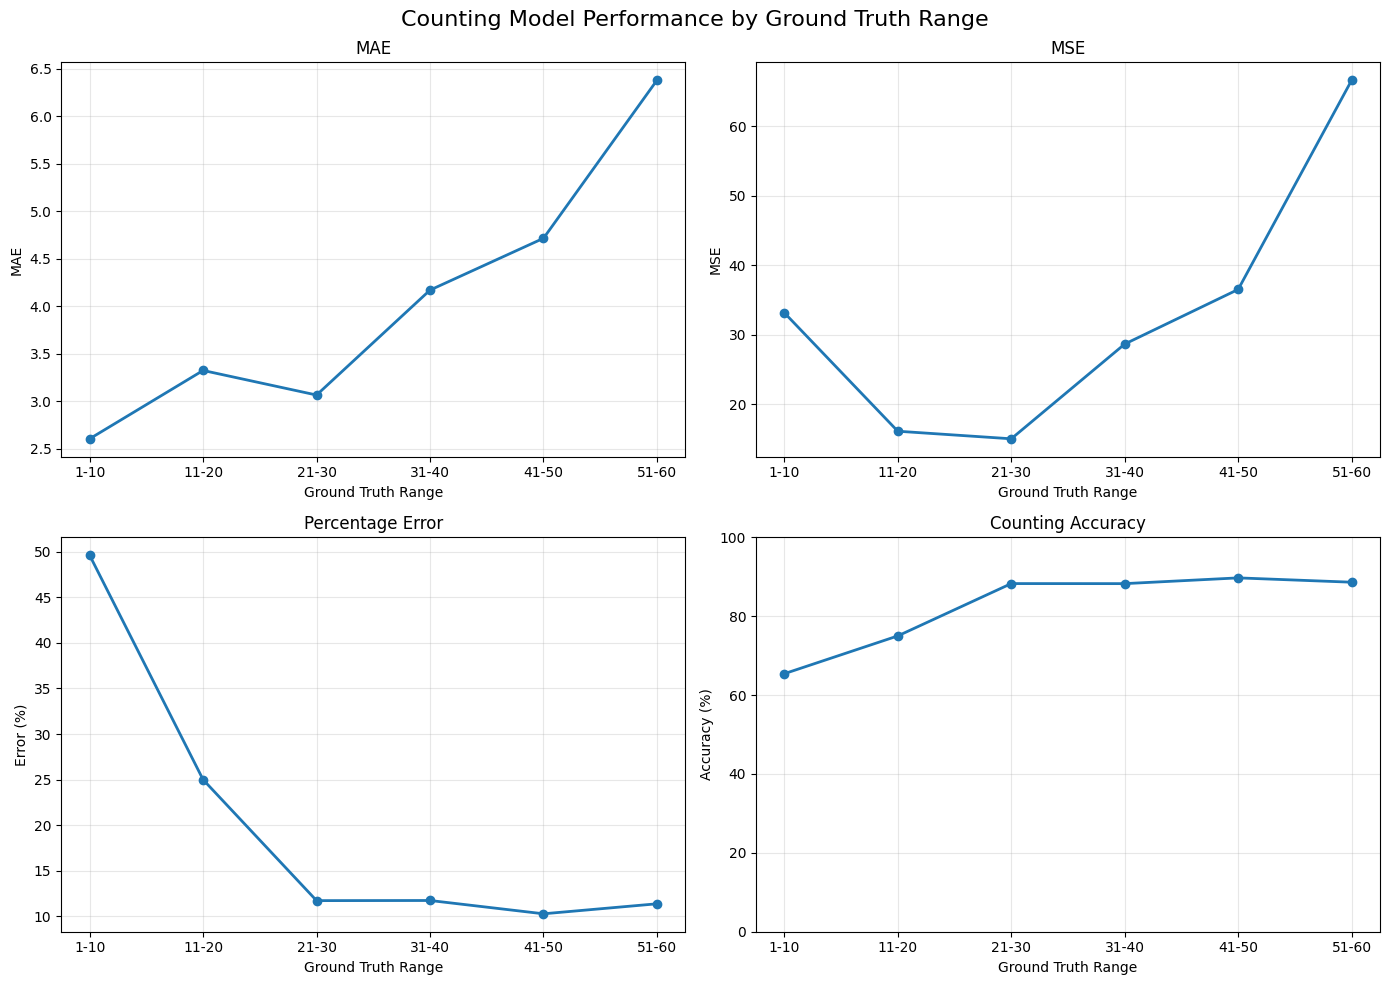
\includegraphics[width=1.0\linewidth]{./../images/scut_head_mcnn/performance_by_gt_range.png}
	\caption{Hybrid YOLO+MCNN metrics across ground truth count ranges}
	\label{fig:hybrid_mcnn_range_metrics}
\end{figure}

\begin{longtable}{|
    >{\raggedright\arraybackslash}p{0.12\textwidth}|
    >{\centering\arraybackslash}p{0.04\textwidth}|
    >{\centering\arraybackslash}p{0.10\textwidth}|
    >{\centering\arraybackslash}p{0.10\textwidth}|
    >{\centering\arraybackslash}p{0.10\textwidth}|
    >{\centering\arraybackslash}p{0.18\textwidth}|
    >{\centering\arraybackslash}p{0.14\textwidth}|
    >{\centering\arraybackslash}p{0.10\textwidth}|
}
\caption{Hybrid YOLO+MCNN performance by ground-truth count range}
\label{tab:hybrid_range_breakdown} \\
\hline
\textbf{GT Range} & \textbf{$n$} & \textbf{MAE} & \textbf{RMSE} &
\textbf{Mean \% Error} & \textbf{Mean Acc.\ (\%)} & \textbf{Mean Bias} \\
\hline
\endfirsthead

\multicolumn{7}{|c|}%
{\tablename\ \thetable{} -- continued from previous page} \\
\hline
\textbf{GT Range} & \textbf{$n$} & \textbf{MAE} & \textbf{RMSE} &
\textbf{Mean \% Error} & \textbf{Mean Acc.\ (\%)} & \textbf{Mean Bias} \\
\hline
\endhead

\hline
\multicolumn{7}{|c|}{Continued on next page} \\
\hline
\endfoot

\hline
\endlastfoot

1--10
& 61
& \textbf{2.6054}
& 5.7591
& 49.6098
& 65.4236
& 0.0211 \\
\hline

11--20
& 48
& 3.3250
& 4.0183
& 24.9948
& 75.0052
& $-0.7383$ \\
\hline

21--30
& 40
& 3.0662
& \textbf{3.8806}
& 11.7258
& 88.2742
& 1.1992 \\
\hline

31--40
& 42
& 4.1714
& 5.3547
& 11.7395
& 88.2605
& 0.6557 \\
\hline

41--50
& 49
& 4.7169
& 6.0433
& \textbf{10.2810}
& \textbf{89.7190}
& 2.1349 \\
\hline

51--60
& 45
& 6.3811
& 8.1594
& 11.3780
& 88.6222
& $-0.5029$ \\
\hline

\end{longtable}

As with the individual models, absolute error broadly increases with ground-truth crowd size while relative (percentage) error decreases, and mean counting accuracy is highest in the moderate-to-high density ranges. The RMSE in the sparsest range (1--10) is disproportionately large relative to its MAE, indicating that a small number of large outlier errors dominate this bin. The lowest MAE is achieved in the 1--10 range, while the lowest RMSE occurs in the 21--30 range, reflecting that the sparsest bin combines many very small errors with a few large outliers; the 41--50 range achieves both the lowest mean percentage error and the highest mean counting accuracy. In the 21--50 range the hybrid framework achieves relative errors broadly comparable to the fine-tuned detector alone, consistent with the observation in Table~\ref{tab:hybrid_mcnn_component_comparison} that the two are closely matched overall, with the detector retaining a modest edge.

\subsection{Hybrid Adaptive Counting: SCUT-Head YOLO Combined with CSRNet}
\label{sec:hybrid_csrnet}

This Section~\ref{sec:fusion} introduces and evaluates an adaptive fusion framework that combines the fine tuned SCUT-Head YOLO detector with a density regression estimate, using CSRNet (Section~\ref{sec:csrnet}) as the density based component. CSRNet is independently trained and evaluated on the same 285-image test set. The same fusion rule is applied to combine the YOLO detection based count with the CSRNet density estimate, providing a consistent evaluation of the resulting hybrid counting framework under the same experimental conditions.

\subsubsection{Quantitative Performance Evaluation}

Table~\ref{tab:hybrid_csrnet_summary} reports the aggregate performance of the SCUT-Head YOLO + CSRNet hybrid on the 285-image test set. It provide an overall view of the hybrid model's counting behaviour across the complete test set. In particular, the difference between the total ground truth count and total predicted count indicates a tendency toward undercounting, while the MAE and RMSE quantify the average and larger counting deviations, respectively. 

\begin{longtable}{|
>{\raggedright\arraybackslash}p{0.65\textwidth}|
>{\centering\arraybackslash}p{0.27\textwidth}|}

\caption{Hybrid YOLO+CSRNet performance.}
\label{tab:hybrid_csrnet_summary} \\
\hline
\textbf{Metric} & \textbf{Value} \\
\hline
\endfirsthead

\multicolumn{2}{|c|}%
{\tablename\ \thetable{} -- continued from previous page} \\
\hline
\textbf{Metric} & \textbf{Value} \\
\hline
\endhead

\hline
\multicolumn{2}{|c|}{\textit{Continued on next page}} \\
\hline
\endfoot

\hline
\endlastfoot

Images
& 285 \\
\hline

Total Ground Truth
& 8{,}310 \\
\hline

Total Predicted
& 8{,}060.45 \\
\hline

Mean Ground Truth Count
& 29.16 \\
\hline

Mean Predicted Count
& 28.2823 \\
\hline

Mean Absolute Error (MAE)
& 3.6543 \\
\hline

Root Mean Squared Error (RMSE)
& 5.0039 \\
\hline

Mean Absolute Percentage Error (MAPE)
& 19.3959\% \\
\hline

\end{longtable}

The aggregate values show that the hybrid maintains a high degree of agreement with the ground truth counts. However, the lower mean predicted count compared with the mean ground truth count suggests that the hybrid configuration generally underestimates the number of people. The MAE of 3.6543 and RMSE of 5.0039 indicate that, although the typical counting error remains relatively limited, some images produce larger deviations that increase the RMSE. The MAPE of 19.3959\% provides an additional normalized measure of this prediction error across images.

The per-image behaviour of these predictions is shown in Figure~\ref{fig:hybrid_csrnet_actual_predicted}. This visualization complements the aggregate statistics by showing how the prediction error changes from image to image and how closely the predicted counts track the corresponding ground truth counts.

\begin{figure}[htbp]
	\centering
	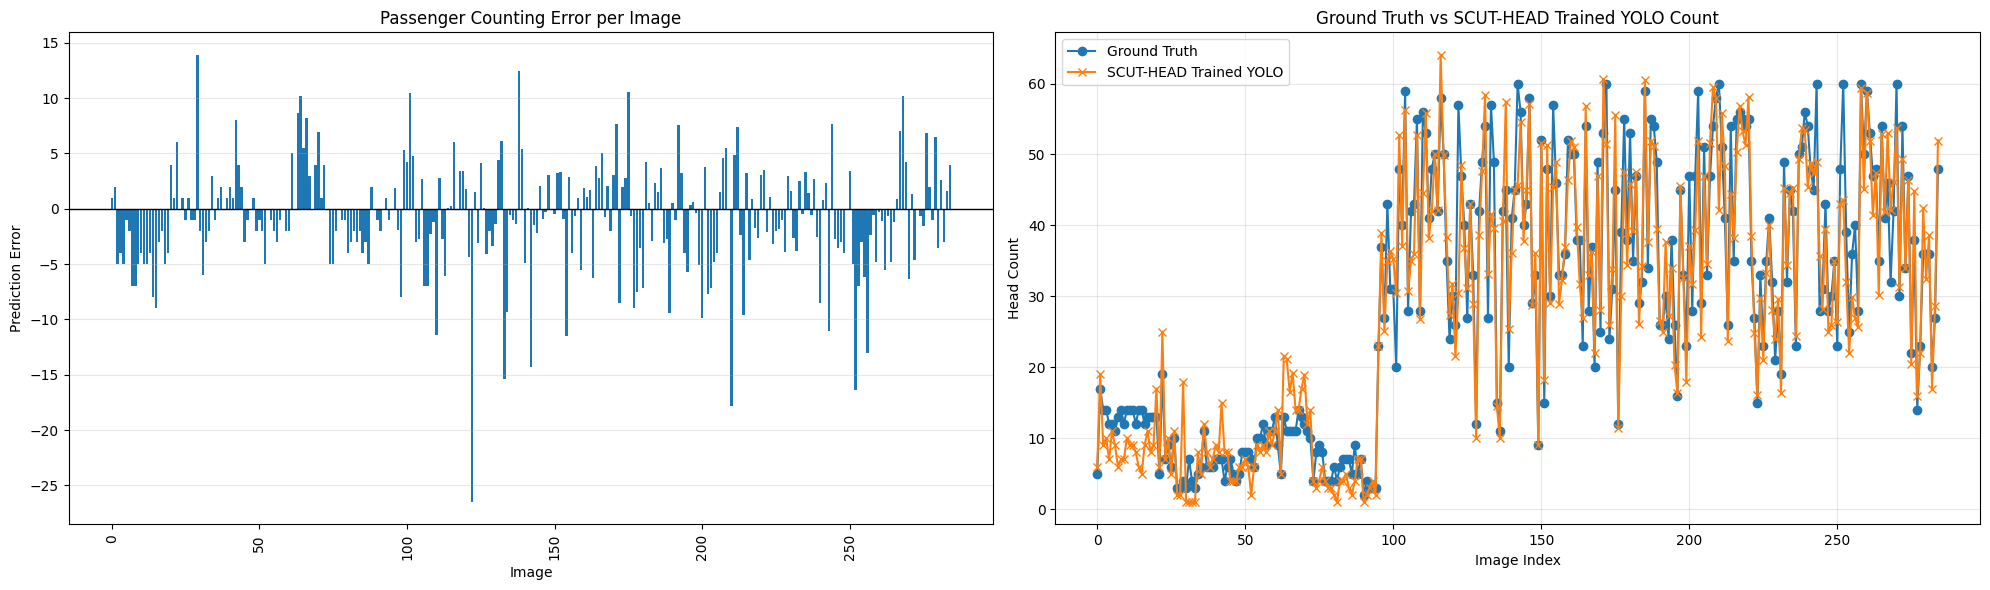
\includegraphics[width=1.0\linewidth]{./../images/scut_head_csrnet/per_image_error_and_gt_vs_predicted.png}
	\caption{Hybrid YOLO+CSRNet counting error and predictions.}
	\label{fig:hybrid_csrnet_actual_predicted}
\end{figure}

Table~\ref{tab:hybrid_csrnet_component_comparison} compares this hybrid configuration against its two constituent models evaluated independently. The component-level comparison is particularly relevant in this case because it shows whether incorporating CSRNet into the stronger SCUT-Head YOLO detector provides any additional counting benefit. It also highlights the extent to which the hybrid configuration preserves the detector's performance while substantially improving upon CSRNet's standalone results.

\begin{longtable}{|>{\raggedright\arraybackslash}p{7.0cm}|
                    >{\centering\arraybackslash}p{2.3cm}|
                    >{\centering\arraybackslash}p{2.3cm}|
                    >{\centering\arraybackslash}p{2.3cm}|}

\caption{Comparison of hybrid YOLO+CSRNet and constituent models.}
\label{tab:hybrid_csrnet_component_comparison} \\
\hline
\textbf{Model} & \textbf{MAE} & \textbf{RMSE} & \textbf{MAPE (\%)} \\
\hline
\endfirsthead

\multicolumn{4}{|c|}%
{\tablename\ \thetable{} -- continued from previous page} \\
\hline
\textbf{Model} & \textbf{MAE} & \textbf{RMSE} & \textbf{MAPE (\%)} \\
\hline
\endhead

\hline
\multicolumn{4}{|c|}{\textit{Continued on next page}} \\
\hline
\endfoot

\hline
\endlastfoot

SCUT-Head YOLO (detector only)
& \textbf{3.2246}
& \textbf{4.3950}
& \textbf{17.0133} \\
\hline

CSRNet (density only)
& 11.8369
& 17.0016
& 120.9659 \\
\hline

Hybrid (SCUT-Head YOLO + CSRNet)
& 3.6543
& 5.0039
& 19.3959 \\
\hline

\end{longtable}

As with the MCNN based hybrid, fusing the detector with CSRNet does not exceed the accuracy of the detector used in isolation, but the gap here is considerably narrower: MAE increases by only 0.4297 (versus 0.7567 for the MCNN based hybrid), RMSE increases by only 0.6089 (versus 1.3451), as shown in Table~\ref{tab:hybrid_csrnet_component_comparison}. At the same time, the hybrid again yields a very large improvement over its density based component used alone, more than halving CSRNet's standalone MAE and RMSE, as shown in Table~\ref{tab:hybrid_csrnet_component_comparison} and illustrated in Figure~\ref{fig:hybrid_csrnet_actual_predicted}.

\subsubsection{Performance by Density Category}

To further evaluate the behaviour of the SCUT-Head YOLO + CSRNet hybrid across different crowd levels, the test images were divided into sparse and dense scene categories. Table~\ref{tab:hybrid_csrnet_density_breakdown} summarizes the counting performance for each category using MAE, RMSE, mean percentage error, mean accuracy, and mean bias.

\begin{longtable}{|>{\raggedright\arraybackslash}p{1.5cm}|
                    >{\centering\arraybackslash}p{1.0cm}|
                    >{\centering\arraybackslash}p{1.2cm}|
                    >{\centering\arraybackslash}p{1.8cm}|
                    >{\centering\arraybackslash}p{2.5cm}|
                    >{\centering\arraybackslash}p{2.5cm}|
                    >{\centering\arraybackslash}p{2.0cm}|}

\caption{Hybrid YOLO+CSRNet performance by scene density.}
\label{tab:hybrid_csrnet_density_breakdown} \\
\hline
\textbf{Density} & \textbf{$n$} & \textbf{MAE} & \textbf{RMSE} &
\textbf{Mean \% Error} & \textbf{Mean Acc.\ (\%)} & \textbf{Mean Bias} \\
\hline
\endfirsthead

\multicolumn{7}{|c|}%
{\tablename\ \thetable{} -- continued from previous page} \\
\hline
\textbf{Density} & \textbf{$n$} & \textbf{MAE} & \textbf{RMSE} &
\textbf{Mean \% Error} & \textbf{Mean Acc.\ (\%)} & \textbf{Mean Bias} \\
\hline
\endhead

\hline
\multicolumn{7}{|c|}{\textit{Continued on next page}} \\
\hline
\endfoot

\hline
\endlastfoot

Sparse
& 146
& \textbf{2.8999}
& \textbf{3.7987}
& 28.2413
& 73.5569
& $-0.7651$ \\
\hline

Dense
& 139
& 4.4467
& 6.0151
& \textbf{10.1053}
& \textbf{89.8947}
& $-0.9917$ \\
\hline

\end{longtable}

As shown in Table~\ref{tab:hybrid_csrnet_density_breakdown}, the density stratified pattern mirrors that of the MCNN based hybrid in its broad shape: absolute error is lower for sparse scenes and higher for dense scenes, while relative error and mean accuracy favour dense scenes. The mean bias is negative in both categories for the CSRNet based hybrid, indicating a persistent, modest tendency to undercount regardless of scene density. This differs from the MCNN based hybrid, whose dense scene bias is positive (an overcounting tendency), showing that the choice of density regression component materially affects the direction of the hybrid's bias in dense scenes even though the overall error pattern by density is similar.

\subsubsection{Performance by Ground Truth Count Range}

To further examine how the SCUT-Head YOLO + CSRNet hybrid performs across different crowd sizes, the test set was divided into ground truth count ranges with a bin width of 10. Figure~\ref{fig:hybrid_csrnet_range_metrics} visualizes the main performance metrics across these ranges, while the detailed numerical results are presented in Table~\ref{tab:hybrid_csrnet_range_breakdown}.

\begin{figure}[htbp]
	\centering
	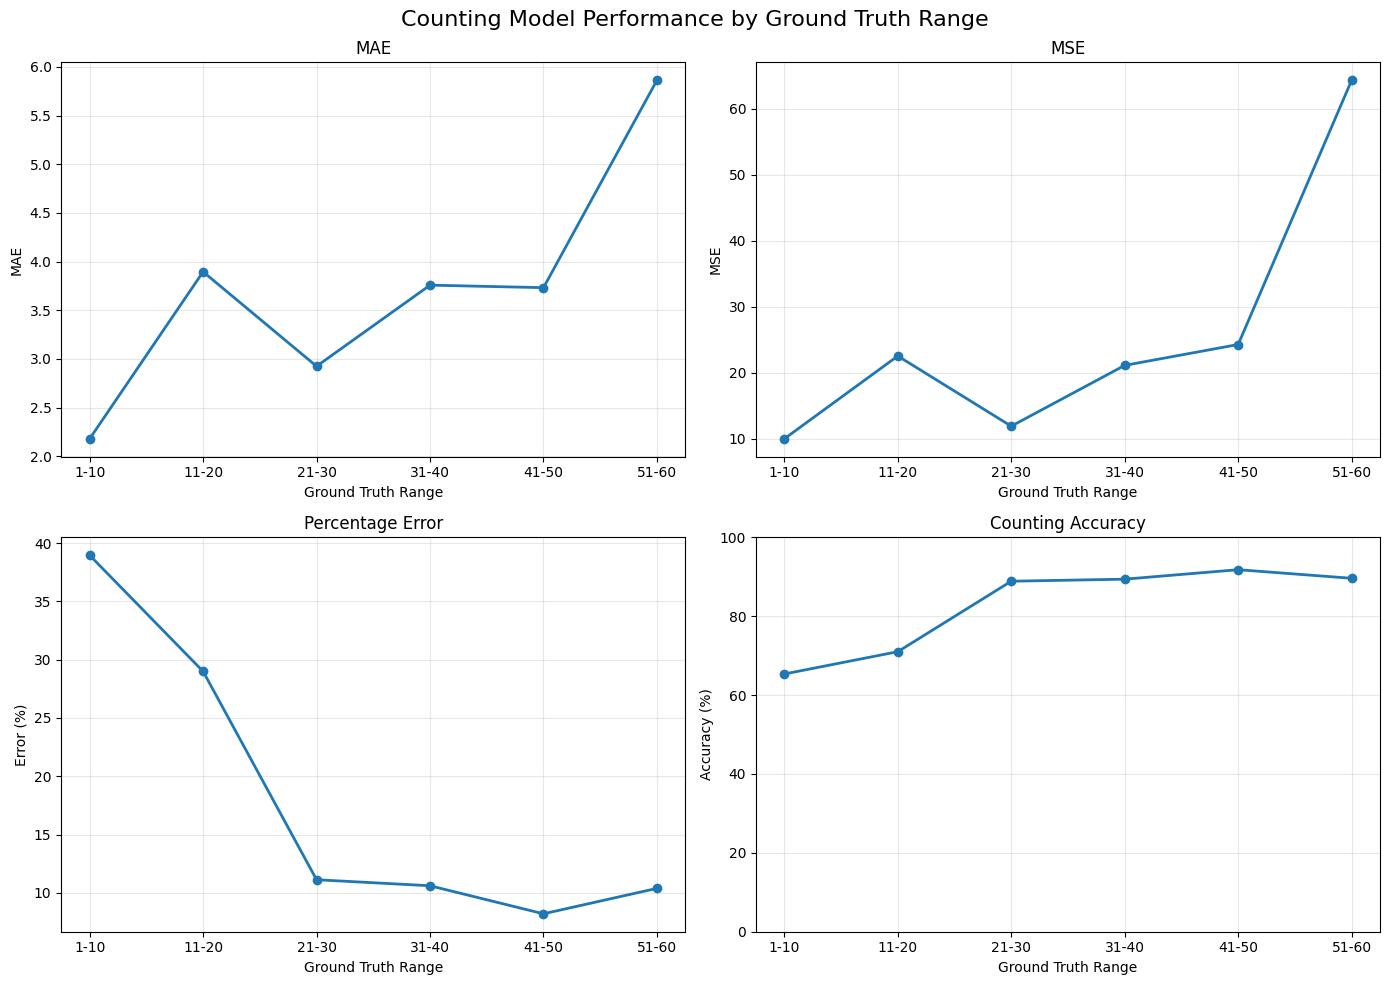
\includegraphics[width=1.0\linewidth]{./../images/scut_head_csrnet/performance_by_gt_range.png}
	\caption{Hybrid YOLO+CSRNet metrics across ground truth count ranges}
	\label{fig:hybrid_csrnet_range_metrics}
\end{figure}

The range-stratified results show the same broad shape as the MCNN based hybrid absolute error rising and relative error falling with crowd size as shown in Table~\ref{tab:hybrid_csrnet_range_breakdown} and Figure~\ref{fig:hybrid_csrnet_range_metrics}. However, there is a notably lower MAE and RMSE in the sparsest range (1--10), where the mean bias (-0.410984) is close to zero and only mildly negative, rather than the small positive bias seen in the same range for the MCNN based hybrid. This is broadly consistent with CSRNet's own range level behaviour (Table~\ref{tab:csrnet_range_breakdown}), which, while still weak in absolute terms, is less prone to the extreme sparse scene overestimation observed for MCNN (Table~\ref{tab:mcnn_range_breakdown}).

\begin{longtable}{|>{\raggedright\arraybackslash}p{1.5cm}|
                    >{\centering\arraybackslash}p{1.0cm}|
                    >{\centering\arraybackslash}p{1.2cm}|
                    >{\centering\arraybackslash}p{1.8cm}|
                    >{\centering\arraybackslash}p{2.5cm}|
                    >{\centering\arraybackslash}p{2.5cm}|
                    >{\centering\arraybackslash}p{2.0cm}|}

\caption{Hybrid YOLO+CSRNet performance by ground truth count range}
\label{tab:hybrid_csrnet_range_breakdown} \\
\hline
\textbf{GT Range} & \textbf{$n$} & \textbf{MAE} & \textbf{RMSE} &
\textbf{Mean \% Error} & \textbf{Mean Acc.\ (\%)} & \textbf{Mean Bias} \\
\hline
\endfirsthead

\multicolumn{7}{|c|}%
{\tablename\ \thetable{} -- continued from previous page} \\
\hline
\textbf{GT Range} & \textbf{$n$} & \textbf{MAE} & \textbf{RMSE} &
\textbf{Mean \% Error} & \textbf{Mean Acc.\ (\%)} & \textbf{Mean Bias} \\
\hline
\endhead

\hline
\multicolumn{7}{|c|}{\textit{Continued on next page}} \\
\hline
\endfoot

\hline
\endlastfoot

1--10
& 61
& \textbf{2.1792}
& \textbf{3.1598}
& 38.9541
& 65.3498
& $-0.4110$ \\
\hline

11--20
& 48
& 3.8954
& 4.7466
& 28.9948
& 71.0052
& $-0.3458$ \\
\hline

21--30
& 40
& 2.9245
& 3.4490
& 11.1258
& 88.8742
& 0.4460 \\
\hline

31--40
& 42
& 3.7581
& 4.5944
& 10.6088
& 89.3912
& $-0.3910$ \\
\hline

41--50
& 49
& 3.7322
& 4.9265
& \textbf{8.2039}
& \textbf{91.7961}
& $-0.6098$ \\
\hline

51--60
& 45
& 5.8636
& 8.0192
& 10.3851
& 89.6149
& $-3.9871$ \\
\hline

\end{longtable}

\subsection{Selecting the Best Hybrid Configuration}
\label{sec:hybrid_selection}

Sections\ref{sec:hybrid_mcnn} and Section~\ref{sec:hybrid_csrnet} evaluated two candidate hybrid configurations SCUT-Head YOLO combined with MCNN, and SCUT-Head YOLO combined with CSRNet under an identical adaptive fusion rule and on the same 285-image test set. This section compares the two configurations directly across all previously reported criteria in order to select the hybrid best suited for general deployment.

\subsubsection{Aggregate Performance Comparison}

Table~\ref{tab:hybrid_selection_aggregate} compares the two hybrid configurations on overall counting accuracy, together with the degradation each incurs relative to the SCUT-Head YOLO detector used in isolation.

\begin{longtable}{|
>{\raggedright\arraybackslash}p{3.0cm}|
>{\centering\arraybackslash}p{4.0cm}|
>{\centering\arraybackslash}p{4.0cm}|
>{\centering\arraybackslash}p{2.7cm}|}

\caption{Aggregate comparison of the two hybrid configurations}
\label{tab:hybrid_selection_aggregate} \\

\hline
\textbf{Metric} & \textbf{YOLO+MCNN} & \textbf{YOLO+CSRNet} & \textbf{Better Config} \\
\hline
\endfirsthead

\multicolumn{4}{|c|}%
{\tablename\ \thetable{} -- continued from previous page} \\
\hline
\textbf{Metric} & \textbf{YOLO+MCNN} & \textbf{YOLO+CSRNet} & \textbf{Better Config} \\
\hline
\endhead

\hline
\multicolumn{4}{|c|}{\textit{Continued on next page}} \\
\hline
\endfoot

\hline
\endlastfoot

MAE
& 3.9813
& \textbf{3.6543}
& CSRNet \\
\hline

RMSE
& 5.7401
& \textbf{5.0039}
& CSRNet \\
\hline

MAPE (\%)
& 21.7678
& \textbf{19.3959}
& CSRNet \\
\hline

\end{longtable}

As shown in Table~\ref{tab:hybrid_selection_aggregate}, the SCUT-Head YOLO + CSRNet configuration outperforms the SCUT-Head YOLO + MCNN configuration on every aggregate metric, and does so while deviating less from the detector only baseline (Tables~\ref{tab:hybrid_mcnn_component_comparison} and~\ref{tab:hybrid_csrnet_component_comparison}), indicating that CSRNet integrates more cleanly with the detector's predictions than MCNN does. This aggregate picture, however, masks substantial regime dependent variation, examined next.

\subsubsection{Comparison by Scene Density}

Table~\ref{tab:hybrid_selection_density} compares the two configurations stratified by sparse and dense scene category reported for each category in Tables~\ref{tab:hybrid_density_breakdown} and~\ref{tab:hybrid_csrnet_density_breakdown}.

\begin{longtable}{|
>{\raggedright\arraybackslash}p{1.7cm}|
>{\raggedright\arraybackslash}p{2.2cm}|
>{\centering\arraybackslash}p{3.2cm}|
>{\centering\arraybackslash}p{3.5cm}|
>{\centering\arraybackslash}p{2.5cm}|}

\caption{Density stratified comparison of the two hybrid configurations.}
\label{tab:hybrid_selection_density} \\

\hline
\textbf{Density}
& \textbf{Metric}
& \multicolumn{2}{c|}{\textbf{Configuration}}
& \textbf{Better Config} \\
\hline

&
&
\textbf{YOLO+MCNN}
&
\textbf{YOLO+CSRNet}
&
\\
\hline
\endfirsthead

\multicolumn{5}{|c|}%
{\tablename\ \thetable{} -- continued from previous page} \\
\hline
\textbf{Density}
& \textbf{Metric}
& \multicolumn{2}{c|}{\textbf{Configuration}}
& \textbf{Better Config} \\
\hline

&
&
\textbf{YOLO+MCNN}
&
\textbf{YOLO+CSRNet}
&
\\
\hline
\endhead

\hline
\multicolumn{5}{|c|}{\textit{Continued on next page}} \\
\hline
\endfoot

\hline
\endlastfoot

Sparse
& MAE
& \textbf{2.6928}
& 2.8999
& \textbf{MCNN} \\
\hline

Sparse
& RMSE
& \textbf{3.5333}
& 3.7987
& \textbf{MCNN} \\
\hline

Sparse
& Mean Bias
& $-0.9154$
& \textbf{$-0.7651$}
& \textbf{CSRNet} \\
\hline

Dense
& MAE
& 5.2428
& \textbf{4.4467}
& \textbf{CSRNet} \\
\hline

Dense
& RMSE
& 7.2792
& \textbf{6.0151}
& \textbf{CSRNet} \\
\hline

Dense
& Mean Bias
& 1.7528
& \textbf{$-0.9917$}
& \textbf{CSRNet} \\
\hline

\end{longtable}

The completed comparison shows that MCNN's sparse scene advantage is broader than absolute error alone: MCNN achieves lower MAE, lower RMSE, lower mean percentage error, and higher mean accuracy in sparse scenes, losing to CSRNet only on bias magnitude, where CSRNet's smaller undercount ($-0.7651$ vs.\ $-0.9154$) is a comparatively minor distinction. In dense scenes, CSRNet wins every metric without exception, including MAE, which is decisive on its own and not merely a byproduct of its RMSE and MAPE advantage. The two configurations therefore occupy genuinely different regimes: MCNN is the more consistently accurate choice in sparse scenes, while CSRNet is unambiguously superior once crowds become dense.

\subsubsection{Comparison by Ground Truth Count Range}

Table~\ref{tab:hybrid_selection_range} extends the range stratified comparison for the fixed Scut-Head-YOLO configuration in sparse scenes, as reported in Tables~\ref{tab:hybrid_range_breakdown} and Table~\ref{tab:hybrid_csrnet_range_breakdown}, by providing a direct comparison of the MAE and RMSE performance of the two hybrid configurations across different ground-truth count ranges.

\begin{longtable}{|
>{\raggedright\arraybackslash}p{1.6cm}|
>{\centering\arraybackslash}p{2.0cm}|
>{\centering\arraybackslash}p{2.0cm}|
>{\centering\arraybackslash}p{2.0cm}|
>{\centering\arraybackslash}p{2.0cm}|
>{\raggedright\arraybackslash}p{3.5cm}|}

\caption{Range stratified comparison of the two hybrid configurations using MAE and RMSE.}
\label{tab:hybrid_selection_range} \\

\hline
\textbf{GT Range}
& \textbf{MAE}
& \textbf{MAE}
& \textbf{RMSE}
& \textbf{RMSE}
& \textbf{Better Config} \\
\hline

& \textbf{MCNN}
& \textbf{CSRNet}
& \textbf{MCNN}
& \textbf{CSRNet}
& \\
\hline
\endfirsthead

\hline
\textbf{GT Range}
& \textbf{MAE}
& \textbf{MAE}
& \textbf{RMSE}
& \textbf{RMSE}
& \textbf{Better Config} \\
\hline

& \textbf{MCNN}
& \textbf{CSRNet}
& \textbf{MCNN}
& \textbf{CSRNet}
& \\
\hline
\endhead

\hline
\textit{Continued on next page}
& & & & & \\
\hline
\endfoot

\hline
\endlastfoot

1--10
& 2.6054
& \textbf{2.1792}
& 5.7591
& \textbf{3.1598}
& CSRNet \\
\hline

11--20
& \textbf{3.3250}
& 3.8954
& \textbf{4.0183}
& 4.7466
& MCNN \\
\hline

21--30
& 3.0662
& \textbf{2.9245}
& 3.8806
& \textbf{3.4490}
& CSRNet \\
\hline

31--40
& 4.1714
& \textbf{3.7581}
& 5.3547
& \textbf{4.5944}
& CSRNet \\
\hline

41--50
& 4.7169
& \textbf{3.7322}
& 6.0433
& \textbf{4.9265}
& CSRNet \\
\hline

51--60
& 6.3811
& \textbf{5.8636}
& 8.1594
& \textbf{8.0192}
& CSRNet \\
\hline

\end{longtable}

The extended range comparison confirms the broad pattern, CSRNet leads on MAE and RMSE in five of six ranges, the exception being 11--20, where MCNN's MAE and RMSE (and, consistently, its Mean \% Error and Mean Accuracy) are meaningfully lower. Two additional patterns emerge once bias and accuracy are included that were not visible from MAE/RMSE alone. First, in the 1--10 range, CSRNet's large MAE/RMSE/MAPE advantage is not unconditional: MCNN's mean bias in this range is close to zero ($+0.0211$) and its mean accuracy is marginally higher than CSRNet's, so CSRNet's win here is driven specifically by fewer large outlier errors rather than a uniformly better per-image fit. Second, and more substantially, in the 51--60 range CSRNet's bias of $-3.9871$ is nearly eight times the magnitude of MCNN's $-0.5029$, despite CSRNet winning MAE, RMSE, MAPE, and accuracy in that bin, indicating that CSRNet's better average absolute error in the highest count range coexists with a systematic, non-trivial undercounting tendency that MCNN does not share there.

\subsubsection{Final Model Selection}

Table~\ref{tab:hybrid_selection_summary} consolidates the comparison into a criterion-by-criterion summary.

\begin{longtable}{|
>{\raggedright\arraybackslash}p{8.0cm}|
>{\centering\arraybackslash}p{3.0cm}|
>{\centering\arraybackslash}p{3.0cm}|}

\caption{Summary of criteria favoring each hybrid configuration.}
\label{tab:hybrid_selection_summary} \\

\hline
\textbf{Criterion}
& \textbf{YOLO+MCNN}
& \textbf{YOLO+CSRNet} \\
\hline
\endfirsthead

\multicolumn{3}{|c|}%
{\tablename\ \thetable{} -- continued from previous page} \\
\hline
\textbf{Criterion}
& \textbf{YOLO+MCNN}
& \textbf{YOLO+CSRNet} \\
\hline
\endhead

\hline
\multicolumn{3}{|c|}{\textit{Continued on next page}} \\
\hline
\endfoot

\hline
\endlastfoot

Aggregate MAE / RMSE / MAPE
&
&
\checkmark \\
\hline

Degradation vs.\ YOLO-only baseline
&
&
\checkmark \\
\hline

Sparse scene Accuracy.
&
\checkmark
& \\
\hline

Sparse scene bias magnitude
&
&
\checkmark \\
\hline

Dense scene Accuracy.
&
&
\checkmark \\
\hline

Dense scene bias magnitude
&
&
\checkmark \\
\hline

\end{longtable}

Weighing the criteria in Table~\ref{tab:hybrid_selection_summary}, the SCUT-Head YOLO + CSRNet configuration is selected as the best performing hybrid framework for general deployment. It dominates every aggregate metric, degrades least relative to the detector only baseline, sweeps all five dense scene metrics without exception, and holds a decisive MAE/RMSE/MAPE advantage in the 1--10 and 21--50 ranges. At the same time, the corrected comparison shows MCNN's case is stronger than the aggregate numbers suggest in two specific regimes: sparse scenes, where MCNN leads on four of five metrics (all but bias), and the 11--20 count range, where MCNN leads on four of five metrics as well (all but bias). CSRNet's own weak point is comparably specific: its bias in the 51--60 range ($-3.9871$) is substantially larger in magnitude than MCNN's ($-0.5029$), even though CSRNet still wins that range on MAE, RMSE, MAPE, and accuracy. SCUT-Head YOLO + CSRNet is therefore adopted as the final hybrid model for subsequent analysis, with the caveat that applications operating primarily on sparse scenes, on crowds in the 11--20 count range, or that are particularly sensitive to systematic bias in the 51--60 range, may warrant reconsidering the MCNN based configuration or a density conditioned choice between the two.
\section{Comparison with Related Work}
\label{sec:related_work}

The SCUT-Head dataset was introduced by Peng et al.~\cite{peng2018scuthead} together with a Feature Refine Net and cascaded multi-scale detection architecture specifically designed for small, densely packed head instances. However, the original publication does not report results in the precision/recall/mAP@50 format used by the Ultralytics YOLO framework employed here, precluding a direct numerical comparison of detection metrics on identical terms. The general finding of that work, namely that head detection in dense, small-instance conditions benefits from architectural provisions for small-object and multi-scale detection, is broadly consistent with the resolution sensitivity directly observed in Section~\ref{sec:scut_yolo}, where a 7.6-point mAP@50 drop was observed when the inference resolution was halved. Nevertheless, this study did not test an architecture specifically designed for small head detection and therefore cannot claim to have reproduced or extended the specific findings of Peng et al. The Multi-Column CNN (MCNN) architecture, which the Four-Column MCNN implementation extends, was introduced by Zhang et al.~\cite{Zhang2016}, who reported a whole-image count MAE of 26.4 on the official ShanghaiTech Part~B \emph{test} set containing 316 images. CSRNet subsequently reported a substantially lower MAE of 10.6 on the same official Part~B test set. Neither published figure is directly comparable to the results presented in Section~\ref{sec:mcnn} and Section~\ref{sec:csrnet}, because both published values represent whole-image count MAE computed on the official 316-image \emph{test} split, whereas the Four-Column MCNN result in this study represents a per-pixel density MAE computed on a 285-image internal dataset that was never evaluated on the official test set. Finally, both the classic and SCUT-Head fine-tuned detectors used in this study are based on the YOLOv8 architecture developed by Ultralytics, which follows the single-shot detection framework introduced by Redmon et al.~\cite{redmon2016yolo}. Since the published COCO benchmarks for YOLOv8 use a different dataset, task, and evaluation protocol, they are not directly comparable with the head-specific SCUT-Head or person-detection results evaluated in this chapter.

\section{Discussion}
\label{sec:discussion}

The results demonstrate the complementary strengths and limitations of detection based and density based crowd counting. Fine tuning the pretrained YOLO detector on SCUT Head substantially improved precision at IoU~0.50 (0.0216 to 0.4449), recall (0.0174 to 0.4273), and MAE (8.8105 to 2.8491). This improvement highlights the importance of adapting a general purpose person detector to head level annotations. However, the fine tuned detector continued to underestimate counts as crowd density increased, indicating that occlusion and overlapping instances remain significant challenges (Table~\ref{tab:scut_head_yolo_range_breakdown}).

Conversely, MCNN and CSRNet exhibited substantial errors in sparse scenes, particularly at counts of 1--10 individuals, but performed more consistently in moderate to high density ranges (Tables~\ref{tab:mcnn_range_breakdown} and~\ref{tab:csrnet_range_breakdown}). Background clutter and visual noise may contribute to sparse scene overestimation, whereas crowd texture provides stronger contextual information in denser scenes. These contrasting error patterns motivated the evaluation of two hybrid configurations combining the fine tuned detector with MCNN or CSRNet.

Both hybrid models substantially reduced density regression errors. The CSRNet based hybrid reduced MAE from 11.8369 to 3.6543, while the MCNN based hybrid reduced it from 14.7544 to 3.9813 (Tables~\ref{tab:hybrid_csrnet_component_comparison} and~\ref{tab:hybrid_mcnn_component_comparison}). Nevertheless, neither configuration outperformed the detector alone. Because the detector was generally more accurate on the evaluated test set, averaging its predictions with noisier density estimates often reduced overall accuracy.

CSRNet proved the more suitable density based component, producing a smaller MAE increase over the detector baseline (0.4297 versus 0.7567 for MCNN; Section~\ref{sec:hybrid_selection}). Its less extreme sparse scene predictions also provided a more reliable fallback when the detector produced zero detections. Overall, the findings support the complementarity of detection and density estimation while demonstrating that hybrid fusion does not necessarily improve aggregate accuracy when one component consistently outperforms the other.

\chapterpage{Conclusion and Future Work}
\mychapter{Conclusion and Future Work}
\label{chap:conclusion}

% \section{Summary of Contributions}
% \label{sec:conclusion_contributions}
This study evaluated detection based and density based crowd head counting methods and investigated their integration into a hybrid framework for public transport imagery. Fine tuned YOLO, MCNN, and CSRNet models were assessed using consistent metrics and density based ground truth ranges. The results highlighted the complementary strengths of detection and density estimation across different crowd densities. Accordingly, an interpretable fusion rule was developed to combine detector based and density regression counts without additional training. Two configurations, SCUT Head YOLO + MCNN and SCUT Head YOLO + CSRNet, were evaluated under identical conditions. The YOLO + CSRNet configuration demonstrated more suitable complementary behaviour, particularly in sparse scenes. The proposed framework was also applied to bus interior images to investigate its potential for passenger occupancy estimation and overcrowding monitoring.

% \section{Limitations}
% \label{sec:conclusion_limitations}
Despite these findings, several limitations remain. The evaluation dataset has limited diversity and may not represent real world conditions such as extremely dense crowds, low light environments, and unusual camera angles. Furthermore, fusion thresholds were determined using evaluation images rather than an independent validation set, leaving their generalisation to unseen data uncertain. Detection accuracy may also decrease when passengers are heavily occluded by other passengers or bus structures. Additionally, the models were evaluated on individual images rather than video sequences, while inference latency, memory usage, and power consumption were not assessed.

% \section{Future Work}
% \label{sec:conclusion_future_work}
Future work should improve the framework's generalisation, reliability, and deployment readiness. A learned decision mechanism could replace the fixed fusion threshold to select the more reliable counting method dynamically. Evaluation should be extended to larger, more diverse bus datasets covering different vehicles, camera positions, lighting conditions, and crowd densities, with independent data used to validate the fusion strategy. Video based experiments could incorporate temporal information and object tracking to improve counting stability across frames. Fine tuning the detector on bus specific images containing occlusions from seats, poles, and handrails may further improve detection accuracy. Finally, computational efficiency should be assessed on representative edge devices by measuring inference latency, memory usage, and power consumption, while exploring quantisation and pruning where necessary.

% ==================================================
% References
% ==================================================
\begingroup
\let\clearpage\relax
\renewcommand{\bibname}{References}
\bibliographystyle{IEEEtran}
\bibliography{references}
\endgroup

\end{document}